\documentclass[12pt,a4paper,notitlepage]{report}
\usepackage[utf8]{inputenc}
\usepackage[left=2cm,top=2cm,right=3cm,bottom=3.0cm,nohead]{geometry}
\usepackage{physics}
\usepackage[english, brazil]{babel}
\usepackage{graphicx}
\usepackage{mathtools}
\usepackage{mathrsfs}
\usepackage[dvips]{color}
\usepackage{newlfont}
\usepackage{caption}
\usepackage{bbm}
\usepackage{amssymb}
\usepackage{indentfirst}
\usepackage{bbold}
\usepackage{epstopdf}
\usepackage[bottom]{footmisc}
\usepackage{comment}
\usepackage{cite}
\usepackage{setspace}
%\usepackage[nottoc,numbib]{tocbibind}
\usepackage[tocflat]{tocstyle}
\usetocstyle{standard}
\DeclareMathOperator\arctanh{arctanh}

\makeatletter
\renewcommand*\env@matrix[1][\arraystretch]{%
  \edef\arraystretch{#1}%
  \hskip -\arraycolsep
  \let\@ifnextchar\new@ifnextchar
  \array{*\c@MaxMatrixCols c}}
\makeatother

\pagenumbering{roman}
\begin{document}


\newcommand{\be}{\begin{eqnarray}}
\newcommand{\ee}{\end{eqnarray}}
\newcommand{\eq}[1]{\begin{align}#1\end{align}}
\newcommand{\Unit}{\mathbb{1}}
\newcommand{\Hop}{\mathcal{H}}
\newcommand{\sinc}{\mbox{ sinc}}
\newcommand{\overbar}[1]{\mkern 1.5mu\overline{\mkern-1.5mu#1\mkern-1.5mu}\mkern 1.5mu}

\begin{titlepage} % 1st
\begin{center}
\vspace{2cm}
\text{UNIVERSIDADE FEDERAL DO PARANÁ}\\[.5cm]
%\text{\large \textbf{Programa de Pós-Graduação em Física}}\\[1.5cm]

\vspace{4cm}

\text{NICHOLAS GANZ ENGELBERT}\\[2cm]

\vspace{3.5cm}

QUANTUM RESOURCES AND QUANTUM IRREALISM \\[.2cm]
IN LORENTZ-BOOSTED FRAMES
\\[2.5cm]

\hfill

\vfill

CURITIBA - PR

2022

\end{center}
\end{titlepage}

\begin{titlepage} %2nd
\begin{center}

\vspace{4cm}

\text{NICHOLAS GANZ ENGELBERT}

\vspace{7cm}

QUANTUM RESOURCES AND QUANTUM IRREALISM \\[.2cm]
IN LORENTZ-BOOSTED FRAMES
\\[2.5cm]

\vspace{2cm}

\hspace{.45\textwidth} % posicionando a minipage
\begin{minipage}{.5\textwidth}
{\footnotesize Dissertação apresentada ao Programa de Pós-graduação em Física do 
Setor de Ciências Exatas da Universidade Federal do Paraná, 
como parte dos requisitos necessários à obtenção do grau de Mestre
em Física. \\[.5cm]
Orientador: Prof. Doutor Renato Moreira Angelo.}
\end{minipage}

\vfill

CURITIBA - PR

2022

\end{center}
\end{titlepage}

\selectlanguage{brazil}
\renewcommand\abstractname{{\footnotesize RESUMO}}
\begin{abstract}
\vspace{.8cm}
    Motivado pelos avanços tecnológicos da computação quântica, o estudo da informação quântica e recursos quânticos tem, nas últimas décadas, alcançado os limites da relatividade especial. No regime relativístico, descobriu-se que o emaranhamento entre os graus de liberdade interno (spin) e externo (momento) de uma única partícula não é invariante sob transformações de Lorentz para referenciais em movimento ({\it boosts de Lorentz}), i.e., essas quantidades podem ser vistas descorrelacionadas em um referencial, mas apresentar correlações quânticas em um outro referencial inercial. Neste trabalho, damos outro passo nas investigações de informação quântica relativística, trazendo à discussão a questão do realismo, de grande interesse fundacional. Em particular, buscamos entender se os elementos de realidade (descritos por Einstein, Podolsky e Rosen\cite{epr_1935}, posteriormente definidos rigorosamente por Bilobran e Angelo\cite{bilobran_angelo_2015}) são invariantes relativísticos, e fornecer uma descrição detalhada sobre como as transformações de Lorentz afetam o realismo de spin e momento.


\vspace{1pt}
\hspace{-15pt}{\bf Palavras-chave:} Boost de Lorentz. Recursos quânticos. Realismo.
\end{abstract}
\thispagestyle{empty}

\newpage


\selectlanguage{english}
\renewcommand\abstractname{{\footnotesize ABSTRACT}}
\begin{abstract} 
\vspace{.8cm}
Driven by the technological advancements of quantum computation, the study of quantum information and quantum resources has, for the past couple of decades, reached the limits of special relativity. In the relativistic regime, it was found that the entanglement between a single particle's internal (spin) and external (momentum) degrees of freedom is not invariant under Lorentz transformations to moving frames ({\it Lorentz boosts}); i.e., these quantities may be uncorrelated in one reference frame, but present quantum correlations in a different inertial frame. In this work, we take the investigations of relativistic quantum information a step further, bringing in the foundationally interesting question of realism to the discussion. In particular, we aim to understand whether or not the elements of reality (first described by Einstein, Podolsky and Rosen\cite{epr_1935}, later rigorously defined by Bilobran and Angelo\cite{bilobran_angelo_2015}) are relativistic invariants, and furnish a detailed description of how Lorentz transformation affect the realism of spin and momentum.

\vspace{1pt}
\hspace{-15pt}{\bf Keywords:} Lorentz boost. Quantum resources. Realism.
\end{abstract}

\thispagestyle{empty}

\renewcommand\listfigurename{{\footnotesize \centerline{LIST OF FIGURES}}}

\cleardoublepage
\begingroup
\makeatletter
\let\ps@plain\ps@empty
\makeatother

\pagestyle{empty}
\listoffigures
\cleardoublepage
\endgroup

\renewcommand\contentsname{{\footnotesize \centerline{CONTENTS}}}


\cleardoublepage
\begingroup
\makeatletter
\let\ps@plain\ps@empty
\makeatother

\pagestyle{empty}
\tableofcontents
\cleardoublepage
\endgroup


\chapter{Introduction}
\setcounter{page}{1}
\pagenumbering{arabic}

Quantum Mechanics (QM), widely regarded as one of the most succesful scientific theories due to its abundant experimental validations and technological developments, remains subject to controversy and debate over what it actually says about the universe. Einstein was perhaps the most famous and earliest critic of the theory, raising pertinent questions that went straight to the heart of what made QM hard to digest. His discussions with Bohr regarding the completeness of QM \cite{epr_1935, bohr_1935} have been considered seminal works to the quantum foundations research program, which is still active to this day. Of all the developments this area of research brought about, one of the most remarkable was Bell's theorem \cite{bell_1964}, which unearthed the role of nonlocality in QM.
Much like Einstein, Bell showed how to properly ask foundational questions and address the alleged issues of quantum theory, in a way that had a lasting impact on the community.

More recently, the prospect of further technological advancements in the field of quantum computation has renewed the interest on quantum reasearch, especially within the context of quantum information. The predominant view among this trendy research front is that QM is, beyond a theory of particles and/or waves, a theory about information: quantifying the information content of physical systems, describing the flow of information between systems and, perhaps most importantly, investigating the ways in which this information can be used for computational tasks. One particular property, exclusive to the quantum realm, which makes quantum computers vastly superior to their classical counterpart is entanglement\cite{horodecki_2009}. When two quantum systems interact, the joint description of their state may present statistical correlations which are unexplainable in classical terms. This phenomena was known since the early days of the theory; in fact, it was instrumental for one of Einstein's strongest arguments against QM, as well as for Bell's theorem. Within quantum information, quantum resource theories \cite{chitambar_2019} are mainly interested in the utility that a particular quantum feature can bring to an information processing task. In this context, entanglement is often regarded as the prime example of a quantum resource.

In the last couple of decades, investigations on quantum foundations and quantum information have extended to the limits of high velocities and energies, reaching the scope of special relativity. The fusion of QM with special relativity is not such a recent development: both theories were born at around the same time, and it didn't take long for their combination to give rise to Quantum Field Theory (QFT). To this day, QFT's description of nature is regarded as the most complete and thorough picture of the fundamental workings of the universe.
However, QFT and its use of fields as fundamental building blocks of nature do not converse well with the standard framework and methods of quantum information and quantum computation. This does not mean that these subjects cannot be properly studied in a relativistic setting.

In 2002, Peres et al \cite{peres2002} published the seminal work of what came to be known as relativistic quantum information \cite{peres_2004}. Their central result was that, under a Lorentz boost (i.e., a transformation to a moving reference frame), the spin of a particle may become entangled to its momentum. This sparked a multitude of related developments, which explored not only the single particle case \cite{alsing_milburn_2002, czachor_2005, dunningham_palge_vedral_2009, saldanha_vedral_2012, saldanha_vedral_2013, taillebois_avelar_2013, matsas_2019, bittencourt_2020, bernardini_bittencourt_2020} but also the consequences of the effect on entanglement between two or more particles \cite{gingrich_adami_2002, jordan_2007, chakrabarti_2009, friis_2010, choi_2011, palge_dunningham_2015, palge_2018, bittencourt_2018, fan_li_2018}, including the boost effects on Bell inequality violations \cite{czachor_1997, lee_young_2004, caban_2005, kim_son_2005, brukner_2021}. Within this context came many alternative propositions for an adequate relativistic spin observable \cite{lee_young_2004, grobe_2014, grobe_2014_2, brukner_2019spin} and relativistic reduced spin density matrix \cite{gonera_2004, taillebois_avelar_2013}.

At the heart of the strange entangling effects of the boost is the Thomas-Wigner rotation \cite{thomas_1926, wigner_1939}. It is a well known (albeit paradoxical) consequence of special relativity that the composition of two non-collinear Lorentz boosts is equivalent to a boost plus a rotation (the Thomas-Wigner rotation). As we will see in detail, this effect plays a crucial role in the transformation law of the spin state of single particle systems. This was relatively well understood within the QFT lore, but its consequences for entanglement and quantum information had been unexplored until the early 2000's.

The immediate guess for the most suitable framework to describe quantum-relativistic fermions is the Dirac equation. As some textbooks on the subject explain \cite{sakurai, drell}, this was initially thought to be the relativistic version of Schrödinger's equation, whose solutions were to be interpreted as probability amplitudes (a wave function, in the usual sense). The four components of the Dirac spinor would then account for the two-valuedness of the spin-1/2, plus a new two-valuedness for the sign of the energy; a new degree of freedom which would ultimately correspond to the positron, or anti-electron.

Soon into the development of the Dirac theory, some problems became apparent that made the interpretation of the Dirac spinor as a single particle wave function untenable. 
Among these is the fact that, while both negative and positive energies appear as components of the same Hilbert space, in practice there are no positron-electron transitions observed in nature, and no particle can be in a superposition of being an electron and a positron. Not only that, but the positron itself is a positive energy particle. This led to the postulation of the Dirac sea: the controversial idea that the vacuum was in fact a sea of infinite negative energy electrons, whose absence are perceived as the presence of positrons. An even more flagrant problem, for our purposes, is that the 4x4 spinorial representation of a Lorentz boost is non-unitary, which means that probabilities are not conserved under these transformations if the Dirac spinor is in fact a quantum state, from which probabilities are computed in the usual manner.

All of this ceases to be a problem when one imposes canonical commutation relations to the Dirac spinor, promoting it to a quantum operator (as opposed to a wave function). This is the QFT description of the Dirac spinor, which, as we already mentioned, does not sit well with the study of entanglement and quantum resources. Despite these considerations, a minority of works in the relativistic quantum information literature still attempt to treat the Dirac spinor as a state in a Hilbert space \cite{alsing_milburn_2002, choi_2011, bittencourt_2018, alberto_1996, alberto_2011, bernardini_2014, bittencourt_2016}. We will avoid these controversies by adopting a more general framework (not in conflict with the rigorous QFT approach), that deals with states in a Hilbert space subject to constraints imposed by special relativity, e.g. that Lorentz transformations must be unitary, so that probabilities are the same in all inertial frames. This is the approach adopted in the majority of works in relativistic quantum information.

Within this formalism, we shall push the discussion towards topics of more foundational interest. We mentioned Einstein's important role in inciting discussions about the adequacy of quantum theory. His most celebrated work in that direction was his collaboration with Podolsky and Rosen: ``Can Quantum-Mechanical Description of Physical Reality Be Considered Complete?" \cite{epr_1935}, where a strong argument was put forth to defend their view that quantum theory was incomplete. Central to their argument was their sufficient criteria for what they called an element of reality: {\it ``If, without in any way disturbing a system, we can predict with certainty (i.e., with probability equal to unity) the value of a physical quantity, then there exists an element of reality corresponding to that quantity"}. This seemed at the time to be an incursion into philosophical, metaphysical territory, which was not yet common practice for physicists. The concept, however, proved to be quite  useful, not only for the purpose of the EPR argument (which we will explain in more detail in a later section), but also for guiding foundational and interpretational discussions of QM. From the concept of element of reality came the broader concept of realism: the notion that physical quantities possess a certain value, independent of any observation or action upon the system.

More recently, a different criterion for realism (still very much rooted in EPR's premises) was proposed by Bilobran and Angelo (BA)\cite{bilobran_angelo_2015}. Their approach was based on the simple premise that, immediately after a measurement is made, the measured observable is real (has an element of reality associated with it). All of the states considered real by EPR's criterion are also real under BA's criterion, but the converse is not always true. For example, a classical system described statistically would fail to meet EPR's criterion, even though the lack of certainty in the predictions, in this case, would be due to subjective ignorance. As we will see, BA's criterion is fit to distinguish between these two cases: uncertainty due to a subjective lack of information vs. uncertainty due to a fundamental indefinition ({\it irreality}) of the observables involved. 

In this work, we will apply BA's framework to investigate how a Lorentz boost affects the reality of spin and momentum. For this purpose, we will look at systems already studied in the literature of relativistic quantum information (in particular, a particle in a superposition of counter-propagating momentum eigenstates, studied in reference \cite{dunningham_palge_vedral_2009}), but also systems yet unexplored in the literature of relativistic quantum information (in particular, the Mach-Zehnder interferometer). We will utilize the standard tools of quantum information to quantify the (well known) spin-momentum entanglement generated by the boost, as well as the irreality of spin and of each of the four-momentum components. Quantum coherence of spin and momentum will also be analysed, and its close connection to the notion of irreality will be discussed. Finally, a paradoxical situation is conceived in which the effects of the Wigner rotation in the boosted Mach-Zehnder seem to imply different detection probabilities (i.e. different counting of detection events) for the two inertial frames. An operational solution to this paradox is then proposed by considering the fundamental role of spin-momentum entanglement in any spin measurement (as implemented by, e.g., the Stern-Gerlach setup).


The rest of the work is structured as follows. In chapter 2, we review all of the QM that will be of use and relevance to our investigations; the basic rules of the formalism applied to discrete and continuous degrees of freedom; the density matrix formalism to describe statistical mixture and quantum entropies, which quantify the degree of ``mixedness" of a quantum state; the desription of composite systems and the diagnosis of entanglement, with a particular emphasis towards spin-momentum entanglement; the idea of ``realism" as conceived by EPR and the subsequent realism framework developed by BA; finally, we apply much of these concepts in a simple example describing spin-1/2 particles. In chapter 3, we present a brief review of special relativity, with a tendency towards group-theoretical notions; we define the Poincaré group and some of its subgroups, in particular the Restricted Lorentz, from which we can understand the Thomas-Wigner rotation; immediately after that, the rest of the chapter is dedicated to reviewing the standard methods of applying special relativity, in particular boost transformations, to quantum mechanics; this is the part of the theoretical review with most specific relevance to our main investigations. In chapter 4, we turn to the main subject of the work, determining how, as a consequence of the relativistic quantum mechanics framework, entanglement and realism are affected by Lorentz transformations. We start the discussion in a general setting, then proceed to review some of the example systems already studied in the literature; finally, we apply the investigations to the Mach-Zehnder interferometer, a system never before studied in the context of relativistic quantum mechanics, which presents some new and interesting behaviors. In chapter 5 we conclude and discuss the implications of the work.

\pagebreak  
  
\chapter{Quantum mechanical preliminaries}
\label{chap:qm}

In this chapter we will go over the standard formalism of QM: the state vector formalism for discrete-spectrum non-degenerate degrees of freedom; continuous degrees of freedom; the density matrix formalism for mixed states and the quantification of mixedness provided by entropies; the description of composite systems and entanglement; the concept of realism according to EPR and BA; and finally an example of application of most of these ideas for spin-1/2 systems.

\section{The basic quantum formalism}


In QM, the state of a physical system is described by a vector $\ket{\psi}$ in a Hilbert space $\mathcal{H}$ (a complex vector space equipped with an inner product).  A measurable quantity $\mathcal{A}$ is described by a Hermitian (self-adjoint) operator, $A = A^\dagger$ acting on $\mathcal{H}$; its eigenvalues correspond to the possible outcomes of a measurement of $\mathcal{A}$. The requirement of hermiticity ensures that the eigenvalues of $A$ are real (null imaginary part), and that eigenvectors associated with different eigenvalues are mutually orthogonal. This means that the eigenvectors of $A$ form a basis of $\mathcal{H}$, satisfying the completeness relation and orthonormality, respectively:

\eq{\begin{split}
\label{complete-a} &\sum_i \dyad{a_i} = \Unit , \\
&\bra{a_i}\ket{a_j} = \delta_{ij} .
\end{split}
}
%
With this, any general state $\ket{\psi}$ may be expressed as a linear combination of eigenvectors of $A$ (or any other observable):

\eq{ \ket{\psi} = \sum_i c_i \ket{a_i} ,
}
%
with expansion coefficients $c_i \equiv \bra{a_i}\ket{\psi}$. Given a quantum state, statistical predictions can be made regarding the measurement of an observable. For an observable $A$ with spectral decomposition $A = \sum_i a_i A_i$, with projectors ($A_i^2 = A_i$) satisfying completeness ($\sum_i A_i = \Unit$) and orthonormality ($A_iA_j = \delta_{ij}A_i$), the probability to obtain the eigenvalue $a_i$ given a measurement of $A$ over the state $\ket{\psi}$ is given by the Born rule:
%
\eq{\mathfrak{p}(a_i) = \expval{A_i}{\psi} , \label{born-rule}
}
%
and the state, following the measurement, undergoes an abrupt, discontinuous ``collapse":

\eq{ \ket{\psi} \xrightarrow{a_i} \frac{A_i \ket{\psi}}{\sqrt{\ev{A_i}{\psi}}} .
}
%
Given the probabilities \eqref{born-rule}, the average value of $A$ is
%
\eq{\label{avg} \langle A \rangle = \sum_i a_i \mathfrak{p}(a_i) = \sum_i \expval{a_i A_i}{\psi} = \expval{A}{\psi}.}
%
The sum of all probabilities is

\eq{ \sum_i \mathfrak{p}(a_i) &= \sum_i \expval{A_i}{\psi} \nonumber \\
&= \bra{\psi}\left(\sum_i \dyad{a_i}\right)\ket{\psi} \nonumber \\
&= \bra{\psi}\ket{\psi} , \nonumber
}
which shows that all states $\ket{\psi}$ should be normalized to unity, $\bra{\psi}\ket{\psi} = 1$, so as to make QM a consistent statistical theory.

The observable corresponding to the total energy of a closed system is called the Hamiltonian, $H$, and it encodes the time evolution of the system via Schrödinger's equation:

\eq{i \hbar \frac{\partial}{\partial t}\ket{\psi(t)} = H \ket{\psi(t)}.
}
%
The effect of the Schrödinger equation's evolution on the quantum state is equivalent to that of a unitary operator; that is, the relation between the state at a time $t_0$ and at a posterior time $t$ is given by $\ket{\psi(t)} = U(t,t_0)\ket{\psi(t_0)}$, with $U(t,t_0)$ being unitary: $U^\dagger = U^{-1}$, and the solution to $i\hbar \tfrac{\partial}{\partial t}U = HU$. If $H$ is independent of time, then the time evolution operator $U(t)$ is simply the exponential of the Hamiltonian: $U(t,t_0) = e^{-iH(t-t_0)/\hbar}$.

\section{Continuous degrees of freedom: position and momentum}
\label{sec:continuous}

In the last section, we assumed that the Hilbert space had some finite dimension $d=\dim\left(\mathcal{H}\right)$, so that all physical quantities could assume, at most, $d$ different values (the amount of eigenvalues of the corresponding observable), and all states could be represented as a linear combination of $d$ different orthogonal states. It is easy to see how this is not the most general scenario. In physics, we often deal with quantities that have a continuum of possible values, so it is desirable that the quantum description can be applied to those as well. Here we will briefly review the standard methods of describing continuous degrees of freedom, in particular position and momentum, using QM.

The position of a particle over one spatial dimension (say, the x axis of some coordinate system) requires an infinite dimensional Hilbert space $\mathcal{H}_x$ and an observable $X$ that acts on that space. The eigenvalues of $X$ range from $-\infty<x<\infty$, and its eigenvectors $\ket{x}$ satisfy completeness and orthonormality:

\eq{\begin{split}
\label{complete-x} &\int_{-\infty}^{\infty} \dd{x} \dyad{x} = \Unit, \\
&\bra{x}\ket{x'} = \delta(x-x') .
\end{split}
}
%
These relations give the continuous generalization of \eqref{complete-a}. From them, we can immediately find the expression of a general state in $\mathcal{H}_x$, expanded in the eigenbasis of $X$:

\eq{ \ket{\psi} = \int_{-\infty}^{\infty} \dd{x} \psi(x) \ket{x} ,
}
where the expansion coefficients $\psi(x) \equiv \bra{x}\ket{\psi}$ are collectively called the {\it wave function}.

The spectral decomposition of the position operator, $X = \int x \dyad{x} \dd{x}$, suggests dealing with $\dyad{x}\dd{x}$ as ``infinitesimal projectors". This makes it simple to generalize the Born rule \eqref{born-rule}, so as to give an infinitesimal probability element of finding the particle in the vicinity of a particular value $x$:

\eq{ \dd{\mathfrak{p}(x)} &= \bra{\psi}\ket{x}\bra{x}\ket{\psi}\dd{x} \nonumber \\
&= \left|\psi(x)\right|^2 \dd{x} .
}
%
With this, the probability of finding the particle in a finite interval $x \in [a,b]$ is

\eq{ \mathfrak{p}(x\in[a,b]) = \int_a^b \left|\psi(x) \right|^2 \dd{x} .
}
%
Just like in the discrete case, normalization of the probabilities $\int_{-\infty}^{\infty}\mathfrak{p}(x)\dd{x} = 1$ depends on the normalization of the quantum state: $\bra{\psi}\ket{\psi}= \int_{-\infty}^{\infty}\left|\psi(x)\right|^2 \dd{x} = 1$.

Another important operator acts on the Hilbert space $\mathcal{H}_x$, and that is the momentum observable $P_x$, satisfying the canonical commutation relation $[X, P_x] = i\hbar$. Much like $X$'s, its eigenvalues also range from $-\infty < p < \infty$ and its eigenvectors $\ket{p}$ form a complete orthonormal basis of $\mathcal{H}_x$:

\eq{\begin{split}&\int_{-\infty}^{\infty}  \dd{p} \dyad{p} = \Unit , \\
&\bra{p}\ket{p'} =  \delta(p - p') .
\end{split}
}
%
The general state $\ket{\psi}$ can then be written as
%
\eq{\label{psi-P} \ket{\psi} = \int \dd{p} \overbar{\psi}(p) \ket{p} ,
}
%
with $\overbar{\psi}(p)$ being the momentum-space wave function.

The fact that $X$ and $P_x$ do not commute implies that there is no simultaneous eigenbasis to these operators; equivalently, a measurement of one of these observables precludes the knowledge about the other. A state of definite position, for example, is one in which momentum is maximally undefined. The exact relation between the position and momentum basis is $\bra{x}\ket{p} = (2\pi\hbar)^{-1/2} \exp(i x p/\hbar)$, such that $\overbar{\psi}(p)$ is the Fourier transform of $\psi(x)$ (as can be seen by inserting the identity from \eqref{complete-x} into \eqref{psi-P}).

Much like the Hamiltonian operator is the generator of time translations, the momentum operator is the generator of spatial translations. This will be particularly important in the context of special relativity, where we shall make ample use of the momentum basis.


\section{Density Matrices}

The standard formulation of quantum mechanics in terms of state vectors presented so far has its limitations. A more general formulation is given in terms of positive operators of unit trace called {\it density matrices}. The corresponding density matrix of a state vector $\ket{\psi}$ is
%
\eq{\rho = \dyad{\psi}.
}
%
The strenght of the density matrix lies in is its ability to describe statistical mixtures of states.
Given a statistical ensemble in which a fraction $\lambda_j$ of systems are found in the state\footnote{Equivalently, the same state can be thought of as the result of an unreliable preparation procedure which prepares the state $\ket{\psi_j}$ with probability $\lambda_j$.} $\ket{\psi_j}$, the density matrix
%
\eq{\label{mixed-rho} \rho = \sum_j \lambda_j \dyad{\psi_j}
}
%
contains all the relevant statistical information about the system. A state like the one above cannot be written as $\rho = \dyad{\phi}$ for any $\ket{\phi}$, except in the trivial case where all but one of $\lambda_j$ are zero. If that is the case, $\rho$ is a rank one matrix and the state is said to be pure. In contraposition, when the states $\ket{\psi_j}$ form an orthonormal basis and the probability distribution is uniform, $\lambda_j = \frac{1}{d}$ ($d=\dim\mathcal{H}$), then the state simplifies to $\rho = \Unit/d$, and it is said to be maximally mixed.

The Born rule \eqref{born-rule} can be cast in terms of density matrices, taking the form
%
\eq{\label{born-dens} p(a_i) = \Tr(A_i \rho),
}
%
and the average value of $A$ follows a similar generalization:
%
\eq{\label{average-dens} \langle A \rangle = \Tr(A\rho).
}
%
It is easy to see that for a pure state $\rho = \dyad{\psi}$, the above equations reduce to their state-vector counterparts \eqref{born-rule} and \eqref{avg}.
For a mixed state such as in \eqref{mixed-rho}, the above formula for $\langle A \rangle$ gives the expected convex combination of pure state averages
%
\eq{ \langle A \rangle &= \Tr(A\sum_j \lambda_j \dyad{\psi_j}) \nonumber \\
&= \sum_j \lambda_j \expval{A}{\psi_j}.
}
%

As already mentioned, pure states correspond to density matrices of rank one. For many purposes, it is useful to quantify how mixed (i.e., how ``far" from pure) a state is. In this following section, we will discuss a class of functions which fulfill that very purpose.

\subsection{Entropies}
\label{sec:entropies}

In classical information theory, the concept of entropy encapsulates the amount of ``ignorance" associated with a random variable and its probability distribution. Specifically, consider a random variable $X$, which can assume $n$ possible values $x_i$, each associated with a probability $p_i$. Then the Shannon entropy \cite{shannon_1948} of $X$ is given by

\eq{\label{shannon} H(X) = -\sum_i^n p_i \log_2 p_i ,
}
%
and it quantifies the average amount of information (measured in bits) obtained when the value of $X$ is revealed, which explains its interpretation as the amount of ``ignorance", or lack of knowledge, associated with the corresponding probability distribution.

In quantum mechanics, the construct analogous to \eqref{shannon} is the von Neumann entropy:

\eq{\label{von-neumann} S(\rho) = - \Tr\left(\rho \log_2 \rho \right) .
}
%
The connection with the Shannon entropy is not immediately obvious. Recall from \eqref{mixed-rho} that the spectral decomposition of $\rho$ gives the convex combination of pure states composing the ensemble, the eigenstates being the pure states and the eigenvalues $\lambda_i$ being the probabilities associated with each. If we use this diagonal form of $\rho$ for computing the von Neumann entropy, we get

\eq{ S(\rho) = -\sum_i \lambda_i \log_2 \lambda_i ,
}
which is exactly the Shannon entropy of the probability distribution $\lambda_i$. Therefore the von Neumann entropy quantifies the lack of knowledge regarding which pure state the system is in. It takes on its minimal value of zero if and only if $\rho$ is pure, and the maximal value of $\log_2 d$, with $d = \dim{\mathcal{H}}$, for the maximally mixed state $\Unit/d$.
The von Neumann entropy is one of the primitive notions of quantum information theory, essential to define the {\it information} $I(\rho)$ contained in a quantum state:

\eq{ I(\rho) = \log d - S(\rho),
}
%
that is, the information is the complementary notion to the ``ignorance" quantified by the entropy.

In the occasion that $\rho$ has only two non-zero eigenvalues $\lambda_1$ and $\lambda_2$ (for example, a mixed state in a two-dimensional Hilbert space), then $\lambda_2 = 1-\lambda_1$, and it becomes useful to define the {\it binary entropy}:

\eq{\label{binary} h(x) = -x\log_2 x - (1-x)\log_2(1-x) .
}
This is a version of the Shannon entropy that depends on a single parameter, which can be either eigenvalue.

An alternative quantifier of ``how mixed" is a quantum state is the linear entropy:

\eq{ S_L(\rho) = 1 - \Pi(\rho) ,
}
%
where the quantity $\Pi(\rho)\equiv\Tr\left(\rho^2\right)$ is called the {\it purity} of the state. When $\rho$ is pure, $\rho^2 = \rho$; the purity is then equal to its maximal value 1 and the linear entropy is 0 (as it should be for a pure state). For a maximally mixed state, the purity reaches the minimal value of $1/d$, and the linear entropy assumes the corresponding maximal value of $1-1/d$. 

An important property of both of these entropies is unitary invariance. If $U$ is a unitary operator, i.e., $U^\dagger = U^{-1}$, the transformation induced on a density matrix is $\rho \rightarrow U\rho U^\dagger$, and it holds that

\eq{\label{unitary-inv} S(U\rho U^\dagger) = S(\rho),
}
%
for the von Neumann entropy but also for the linear entropy as well. This means that a unitary evolution, such as the time evolution induced by the Schrödinger equation, does not change the amount of knowledge about a quantum state. In terms of information, \eqref{unitary-inv} implies also that $I(U\rho U^\dagger) = I(\rho)$, that is, unitary evolutions do not change the amount of information held in a quantum state.

Both von Neumann and linear entropies serve the same purpose and quantify the same thing, but they don't agree on exact values. This is not a problem, as long as one is a monotonic function of the other (as they are): they agree on the increases and decreases of their values. To illustrate the differences and similarities of both these quantities, consider the following two-dimensional density matrix:

\eq{\label{rhoalpha} \rho_\alpha = \alpha \frac{\Unit_2}{2} + (1-\alpha)\dyad{\psi} ,
}
%
which is a convex combination of the maximally mixed state $\Unit_2/2$ and some pure state $\ket{\psi}$. Figure \ref{entropy-graph} shows a comparative plot of both von Neumann and linear entropies as a function of the parameter $\alpha$, as well as a parametric plot with $S(\rho_\alpha)$ and $S_L(\rho_\alpha)$ in the x and y axes, respectively.

\begin{figure}[t]
  \centering
  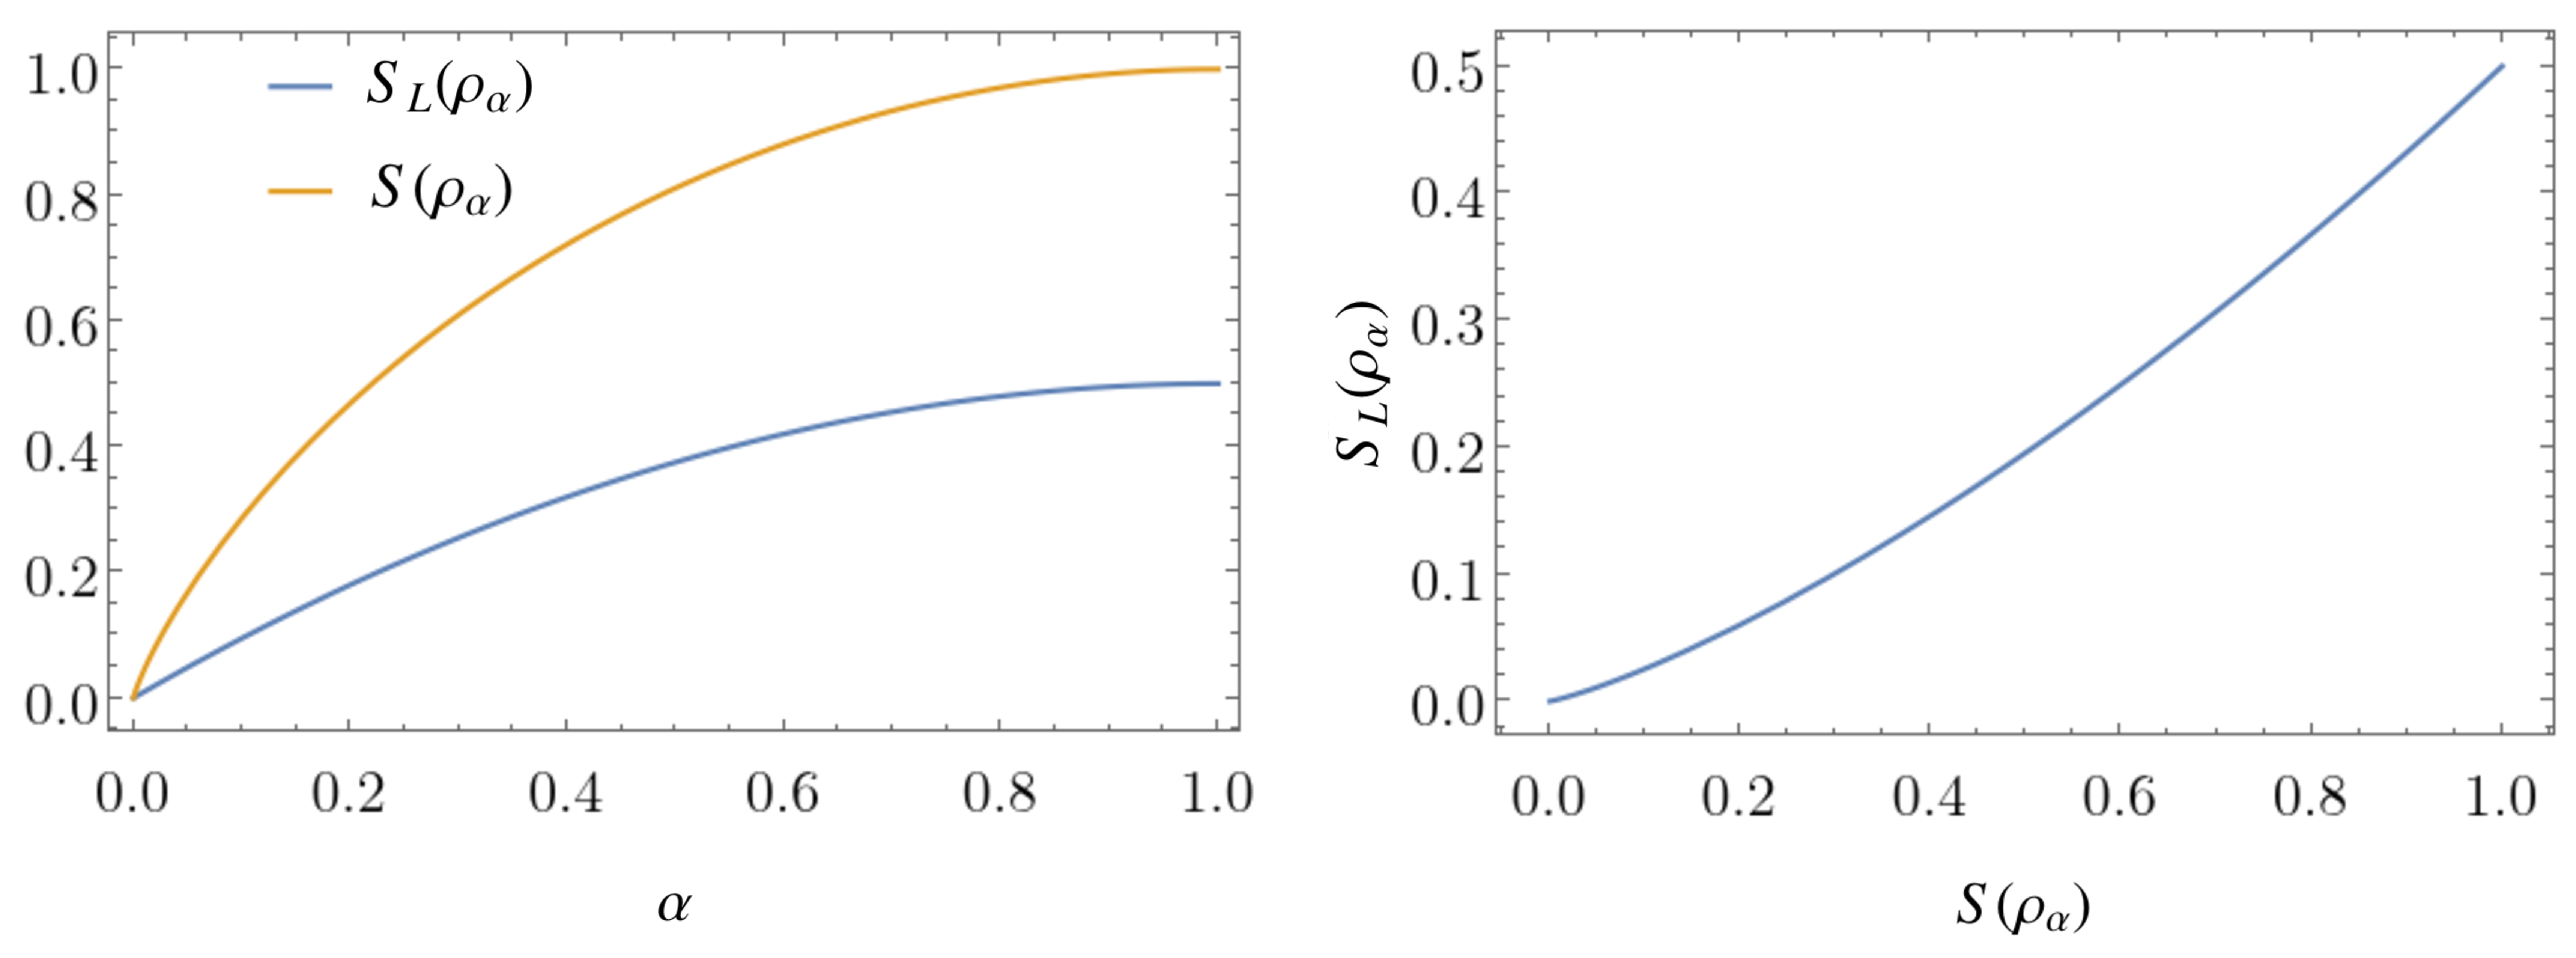
\includegraphics[width=.85\textwidth]{../Figuras/entropias.eps}
  \captionsetup{font=footnotesize, margin=8pt}
  \caption{Left: von Neumann entropy $S(\rho_\alpha)$ and linear entropy $S_L(\rho_\alpha)$ of the state $\rho_\alpha$ (equation \eqref{rhoalpha}) as a function of the parameter $\alpha$. Right: parametric plot showing the monotonicity of both entropies.}
  \label{entropy-graph}
\end{figure}

For some specific purposes later on, the relative entropy will also show up:

\eq{ S(\rho || \sigma) &:= -\Tr(\rho\log_2\sigma) - S(\rho) \nonumber \\
&=  \Tr(\rho(\log_2\rho - \log_2\sigma)) .
}
%
This quantity, which is non-negative, measures the distinguishability of two quantum states $\rho$ and $\sigma$, being zero exclusively when $\rho = \sigma$. It can be seen from its definition that $S(\rho || \sigma) \neq S(\sigma || \rho)$; thus, in some cases, a fairer quantifier of distinguishability is given by the average of these two quantities.


Before moving on, it is worth making a distinction between ``subjective ignorance" and ``objective ignorance". QM is a statistical theory by nature, which means that even if we know the pure state the system is in, the predictions about measurement results are probabilistic. This sort of ignorance (about a measurement performed on a pure state) is what we call ``objective", since it is irreducible and pertains to the most complete description we can coinceive for the system. If, on the other hand, we use (for one reason or the other) a mixed state for describing the system, then there is an additional layer of ignorance, in regards to which pure state the system is in. This is what we call ``subjective ignorance"; the same sort of lack of information which appears in statistical mechanics or classical probability theories. The entropies presented in this section quantify exclusively the subjective ignorance contained in a quantum state.

\section{Composite Systems}
\label{sec:composite}

One reasonable thing to expect from any physical theory is that it should be able to describe larger systems if we know the description of the parts that compose it. Conversely, we should be able to describe and make reference to subsystems of the whole. In QM, these ideas are formalized and made rigorous by the tensor product.

Consider a system $\mathcal{A}$, described by a vector (or density operator) in a Hilbert space $\mathcal{H}_{\mathcal{A}}$ of dimension $d_\mathcal{A}$, and a second system $\mathcal{B}$, described similarly by a Hilbert space $\mathcal{H}_{\mathcal{B}}$ of dimension $d_\mathcal{B}$. The joint description of both systems is given by a Hilbert space which is a tensor product of the subsystem spaces: $\mathcal{H}_{\mathcal{AB}} = \mathcal{H}_{\mathcal{A}}\otimes\mathcal{H}_{\mathcal{B}}$, with dimension $d_{\mathcal{AB}} = d_\mathcal{A} d_\mathcal{B}$. If $\{ \ket{\psi_i}_\mathcal{A} \}$, $i = 1, ..., d_\mathcal{A}$ is a basis of $\mathcal{H}_\mathcal{A}$ and $\{\ket{\phi_j}_\mathcal{B} \}$, $j = 1, ..., d_\mathcal{B}$ is a basis of $\mathcal{H}_\mathcal{B}$, then a possible basis of $\mathcal{H}_{\mathcal{AB}}$ is $\{ \ket{\chi_{ij}}_{\mathcal{AB}} = \ket{\psi_i}_\mathcal{A}\otimes \ket{\phi_j}_\mathcal{B} \equiv \ket{\psi_i}\ket{\phi_j}\}$. A general state of the composite system can then be written as

\eq{\label{tensor-product-state} \ket{\psi} = \sum_{i=1}^{d_\mathcal{A}} \sum_{j=1}^{d_\mathcal{B}} c_{ij} \ket{\psi_i}\ket{\phi_j} .
}
%
A state like the one above can present peculiar properties depending on wether or not the coefficients $c_{ij}$ can be decomposed as $c_{ij} = a_ib_j$. This point shall be given more attention later.

Even though this work will be mostly dealing with single particle systems, tensor product spaces still appear when describing different degrees of freedom of the same particle (for example, position and spin). We used spaces of finite dimension to exemplify the tensor product so far, but the same rules hold for the composition of systems (or degrees of freedom) of infinite dimension. In particular, a Hilbert space that describes the three position coordinates of three-dimensional space is given by the tensor product of three infinite dimensional Hilbert spaces:

\eq{ \mathcal{H}_{\vb{r}} = \mathcal{H}_x \otimes \mathcal{H}_y \otimes \mathcal{H}_z ,
}
where each of the three subspaces being composed obey the same principles and rules laid out in section \ref{sec:continuous}. A basis of $\mathcal{H}_{\vb{r}}$ can be made from the eigenstates of the position operator\footnote{Slight abuse of notation. Each component of the vector $\vb{R}$ is an operator on the full Hilbert space $\mathcal{H}_{\vb{r}}$, so the more rigorous expression would be $\vb{R} = (X\otimes\Unit_y\otimes\Unit_z, \Unit_x\otimes Y\otimes\Unit_z, \Unit_x\otimes\Unit_y\otimes Z)$. The same abbreviated notation will be used for the components of the momentum operator.} $\vb{R} = (X, Y, Z)$, $\vb{R} \ket{\vb{r}} = \vb{r} \ket{\vb{r}}$ where $\vb{r} = (x, y, z)$ and $\ket{\vb{r}} \equiv \ket{x}\ket{y}\ket{z}$. In this way, $\ket{\vb{r}}$ forms a complete orthonormal basis of $\mathcal{H}_{\vb{r}}$, meaning
%
\eq{\begin{split} &\int \dd[3]{r} \dyad{\vb{r}} = \Unit, \\
&\bra{\vb{r}'}\ket{\vb{r}} = \delta^3(\vb{r} - \vb{r}'),
\label{completenessR}
\end{split}
}
%
such that a general state of $\mathcal{H}_{\vb{r}}$ can be expressed as $\ket{\psi} = \int \dd[3]{r} \psi(\vb{r})\ket{\vb{r}}$.

As a straightforward generalization of section \ref{sec:continuous}, each of the three coordinates has its corresponding momentum operator, which can be unified into the vector $\vb{P} = (P_x, P_y, P_z)$. It's eigenstates also obey completeness and orthonormality relations analogous to \eqref{completenessR}, and a general state of $\mathcal{H}_{\vb{r}}$ can be expanded as $\ket{\psi} = \int \dd[3]{p} \overbar{\psi}(\vb{p}) \ket{\vb{p}}$. The relation between the position and momentum basis is $\bra{\vb{r}}\ket{\vb{p}} = (2\pi\hbar)^{-3/2} \exp(i \vb{r}\cdot\vb{p}/\hbar)$, such that the relation between the position space wave function $\psi(\vb{r})$ and the momentum space wave function $\overbar{\psi}(\vb{p})$ is given by the three-dimensional Fourier transform:

\eq{ \overbar{\psi}(\vb{p}) = \frac{1}{(2\pi\hbar)^{3/2}}\int \dd[3]{r} \psi(\vb{r}) e^{i \vb{r}\cdot\vb{p}/\hbar} .
}
%
As a final example of composite systems, we will show how to include a particle's spin to the description that already features the three spatial degrees of freedom of $\mathcal{H}_{\vb{r}}$.

Spin is the intrinsic angular momentum of a particle. Equivalently, it can be defined as the angular momentum of the particle when it is at rest, since when $\vb{p}=\vb{0}$ there is no contribution from the orbital angular momentum, $\vb{L} = \vb{r} \times \vb{p} = \vb{0}$. A particle with spin $s$ ($s$ can be an integer or half-integer) has $2s+1$ possible values resulting from the measurement of any given component. Thus, spin is a discrete degree of freedom, described by a Hilbert space $\mathcal{H}_s$ of dimension $2s+1$. A basis of $\mathcal{H}_s$ can be constructed from the eigenstates of any spin component, the conventional choice being the z component $S_z$, for which $S_z \ket{m} = m\hbar \ket{m}$, with $-s \leq m \leq s$. This basis, along with any other spin component's eigenbasis, obey the usual completeness and orthonormality relations,

\eq{\begin{split} &\sum_{m = -s}^{s} \dyad{m} = \Unit, \\
&\bra{m'}\ket{m} = \delta_{m'm},
\label{completenessS}
\end{split}
}
%
and a general state is $\ket{\psi} = \sum_m c_m \ket{m}$, $c_m \equiv \bra{m}\ket{\psi}$.
A full description that includes position (or momentum) and spin is then given by the Hilbert space $\mathcal{H} = \mathcal{H}_{\vb{r}}\otimes \mathcal{H}_{s}$. The states in this space follow a similar form as \eqref{tensor-product-state}, the only difference being that one of the spaces is infinite dimensional. Hopefully by this point it is not hard to notice that a general single particle pure state of the space $\mathcal{H}$ is

\eq{\label{spin-momentum-state} \ket{\psi} = \sum_{m=-s}^{s} \int \dd[3]{p} \psi_m(\vb{p}) \ket{\vb{p}, m},
}
%
where $\ket{\vb{p}, m} \equiv \ket{\vb{p}}\otimes\ket{m}$ and $\psi_m(\vb{p}) \equiv \bra{\vb{p}, m}\ket{\psi}$ is a wave function of $2s+1$ discrete components, corresponding to the probability amplitude of finding the particle with momentum $\vb{p}$ and spin $m$ along the z axis. Since the main object of investigation in this work will be spin-momentum entanglement, it is important that the reader understands and familiarizes themselves with states such as the one above. When we get to the relativistic description, some adaptations will be necessary, but the states will maintain a form very similar to \eqref{spin-momentum-state}.  We will now proceed to define and characterize entanglement, in both a general setting as well as in the spin-momentum partition.



\subsection{Entanglement}
\label{sec:entanglement}

Consider again the state in \eqref{tensor-product-state}. If the coefficents admit a decomposition of the kind $c_{ij} = a_ib_j$, then

\eq{ \ket{\psi} &= \sum_{i=1}^{d_\mathcal{A}} \sum_{j=1}^{d_\mathcal{B}} a_ib_j \ket{\psi_i}\ket{\phi_j} \nonumber \\
&= \left( \sum_{i=1}^{d_\mathcal{A}} a_i \ket{\psi_i} \right) \otimes \left( \sum_{j=1}^{d_\mathcal{B}} b_j \ket{\phi_j} \right) \nonumber \\
&= \ket{\chi}\otimes\ket{\xi} ,
\label{separable}}
%
and each of the subsystems may be associated with a pure state: $\ket{\chi}$ for subsystem A and $\ket{\xi}$ for subsystem B. Needless to say, this is an extremely specific case, and general states don't admit such a decomposition. When they don't, the two degrees of freedom are said to be entangled.

If a general state of a tensor product space is not separable, there are no pure states that accurately describe the subsystems, but that does not mean that {\it no} state may be attributed to them. The subsystem states of an entangled state can be obtained through the partial trace operation. Consider the density matrix associated to the pure state of equation \eqref{tensor-product-state}:

\eq{\nonumber \rho = \dyad{\psi} &= \left( \sum_i \sum_j c_{ij}\ket{\psi_i}\ket{\phi_j} \right)\left(  \sum_k \sum_l c^*_{kl}\bra{\psi_k}\bra{\phi_l}  \right) \\
&= \sum_{ijkl} c_{ij}c^*_{kl} \ket{\psi_i}\bra{\psi_k} \otimes \ket{\phi_j}\bra{\phi_l} .
\label{bipartite-dens-mat}
}
%
If $\{ \ket{a_i} \}$ is a basis of $\mathcal{H}_\mathcal{A}$, then the partial trace of $\rho$ over the subsystem A is

\eq{ \rho_{\mathcal{B}} = \Tr_{\mathcal{A}}(\rho) = \sum_{i=1}^{d_\mathcal{A}} \mel{a_i}{\rho}{a_i} ,
}
%
which is a density operator on $\mathcal{H}_\mathcal{B}$. Like the regular trace, the partial trace is independent of basis. Using the basis $\{ \ket{\psi_i}_\mathcal{A} \}$ to evaluate the partial trace of the state \eqref{bipartite-dens-mat}, we get

\eq{ \rho_{\mathcal{B}} &= \sum_{m} \mel{\psi_m}{\rho}{\psi_m} \nonumber \\
&= \sum_{ijklm} c_{ij}c^*_{kl} \delta_{im}\delta_{km} \ket{\phi_j}\bra{\phi_l} \nonumber \\
&= \sum_{jlm}c_{mj}c^*_{ml} \ket{\phi_j}\bra{\phi_l} .
\label{rhoB}}
%
Analogously, using the basis $\{ \ket{\phi_i}_\mathcal{B} \}$ to evaluate the trace over subsystem B, we get

\eq{ \label{rhoA}  \rho_{\mathcal{A}} = \sum_{ikm}c_{im}c^*_{km} \ket{\psi_i}\bra{\psi_k}.
}
Even though we cannot attribute a state vector to each subsystem when the global state is entangled, the states \eqref{rhoB} and \eqref{rhoA} provide the best possible description of each subsystem. But what do we mean by ``best possible description"? When measuring an observable $A$, with projectors $A_i$, that acts on space $\mathcal{H}_\mathcal{A}$ (i.e. an observable that pertains to subsystem A alone), the corresponding observable that acts on the total Hilbert space is $A\otimes\Unit_\mathcal{B}$, with projectors $A_i\otimes\Unit_\mathcal{B}$. The measurement statistics can then be obtained by eqs. \eqref{born-dens} and \eqref{average-dens}:

\eq{\begin{split} p(a_i) &= \Tr(A_i\otimes\Unit_\mathcal{B} \rho), \\
\langle A \rangle &= \Tr(A \otimes\Unit_\mathcal{B}\rho) .
\end{split}
}
%
The total trace is equivalent to the partial trace over both subsystems. By evaluating first the trace over $\mathcal{H}_\mathcal{B}$, we get

\eq{ \begin{split}
\label{born-reduced} p(a_i) &= \Tr_\mathcal{A}(A_i \Tr_\mathcal{B}(\rho)) = \Tr_\mathcal{A}(A_i \rho_\mathcal{A}), \\
\langle A \rangle &= \Tr_\mathcal{A}(A \Tr_\mathcal{B}(\rho)) = \Tr_\mathcal{A}(A \rho_\mathcal{A}) .
\end{split}
}
%
Thus we see that the reduced density matrix provides the correct statistical predictions for subsystem A without having to consider other subsystems, even if they are entangled. This is what we mean by the ``best possible description" provided by the reduced density matrix.

When $\ket{\psi}$ is separable like in \eqref{separable}, it is easy to verify that $\rho_\mathcal{A} = \dyad{\chi}$ and $\rho_\mathcal{B} = \dyad{\xi}$. When $\ket{\psi}$ is entangled, $\rho_\mathcal{A}$ and $\rho_\mathcal{B}$ will be mixed states. This shows a counterintuitive aspect of quantum correlations: entanglement allows one to have complete knowledge about the ``whole" (zero entropy for the global state), while having incomplete knowledge about the parts that compose it.

Entanglement between the two subsystems A and B is actually quantified by how mixed the reduced density matrix is. This is where the discussions of section \ref{sec:entropies} present their usefulness. In this work we will be dealing exclusively with global states that are pure. Mixed states, and the quantification of ``mixedness" provided by entropies, will still be crucial when considering subsystems of entangled states. The von Neumann entropy of the reduced density matrix is called the {\it entropy of entanglement} of state $\ket{\psi}$:

\eq{ E(\ket{\psi}) = S(\rho_\mathcal{A}) = S(\rho_\mathcal{B}) ,
}
%
and it quantifies the entanglement between the two subsystems. The linear entropy may also be used to the same effect, keeping in consideration their differences and similarities discussed in section \ref{sec:entropies}.

Since the main subject of this work is entanglement between spin and momentum, let's go back to the spin-momentum state of \eqref{spin-momentum-state}:

\eq{ \tag{\ref{spin-momentum-state}} \ket{\psi} = \sum_{m=-s}^{s} \int \dd[3]{p} \psi_m(\vb{p}) \ket{\vb{p}, m} .
}
%
The trivial factorization of the wave function which guarantees that the state above is separable is $\psi_m(\vb{p}) = c_m \phi(\vb{p})$, for some $\{c_m\}$ and $\phi(\vb{p})$ satisfying $\sum_m |c_m|^2 = 1$ and $\int |\phi(\vb{p})|^2 \dd[3]{p} = 1$. If this factorization holds, then
%
\eq{ \ket{\psi} &= \left( \int \dd[3]{p} \phi(\vb{p})\ket{\vb{p}} \right) \otimes \left( \sum_{m=-s}^s c_m \ket{m} \right) \nonumber \\
&= \ket{\phi}\otimes\ket{\sigma}.
}
%
States for which the wave function cannot be decomposed as above are said to be spin-momentum entangled. These states carry statistical correlations between the two degrees of freedom: through a measurement made in one subsystem, it is possible to obtain information about the other. As a rudimentary example of an entangled state consider
%
\eq{ \psi_m(\vb{p}) = \delta(\vb{p}-\vb{p}_m).
}
%
Setting aside some subtleties regarding normalization, the state vector representation of the above state is
%
\eq{\ket{\psi} = \sum_{m=-s}^s  \frac{\ket{\vb{p}_m, m}}{\sqrt{2s+1}},
}
%
from which we can see that a measurement of the spin component $S_z$ also perfectly determines with which of the momenta $\vb{p}_m$ the particle is found.

To quantify entanglement between spin and momentum, we must evaluate the entropy of the reduced state. This could be in principle either the spin reduced density matrix (tracing out the momentum) or the momentum reduced density matrix (tracing out the spin). The momentum density matrix, however, is infinite dimensional, with infinite eigenvalues. This makes it much more useful to deal with the spin reduced density matrix. The pure state density matrix $\rho = \dyad{\psi}$ corresponding to the state \eqref{spin-momentum-state} is

\eq{ \rho &= \left(\sum_{m=-s}^{s} \int \dd[3]{p} \psi_m(\vb{p}) \ket{\vb{p}, m} \right) \left( \sum_{n=-s}^{s} \int \dd[3]{q} \psi^*_n(\vb{q}) \bra{\vb{q}, n} \right) \nonumber \\
&= \sum_{mn}\int \dd[3]{p} \int \dd[3]{q} \psi_m(\vb{p}) \psi^*_n(\vb{q}) \ket{\vb{p}, m}\bra{\vb{q}, n} .
}
%
The spin reduced density matrix, $\rho_S = \Tr_{\vb{p}}(\rho)$, is given by
\eq{\rho_S &= \int \dd[3]{\pi} \expval{\rho}{\vb*{\pi}} \nonumber \\
&= \sum_{mn} \int \dd[3]{\pi} \psi_m(\vb*{\pi})\psi^*_n(\vb*{\pi}) \ket{m}\bra{n} .
}
%
The object resulting from this operation will be a $(2s+1)\times(2s+1)$ matrix containing all the statistical information about the spin of the particle. All of the information regarding the momentum degree of freedom is automatically marginalized when the partial trace is evaluated, so that probabilities and averages can be computed through \eqref{born-reduced}.

\section{Realism}

Ever since its inception, QM has been the subject of endless foundational and interpretational debates. Perhaps the most notorious example, which is often considered to be the beginning of the quantum foundations research program, is the debate between Einstein and Bohr regarding the completeness of quantum theory \cite{epr_1935, bohr_1935}.

In 1935, Einstein, Podolsky and Rosen put forth an argument defending that quantum theory's description of reality must be incomplete.
Central to their argument was a sufficient criterion for what they called an {\it element of reality}, which stated:
%
{\it ``If, without in any way disturbing a system, we can predict with certainty (i.e., with probability equal to unity) the value of a physical quantity, then there exists an element of reality corresponding to that quantity".}
%
In addition to the requirement that all elements of reality must have a counterpart in the physical theory (in this case, QM), by using an entangled state and assuming locality (no faster-than-light influence), EPR were able to conclude that QM must be an incomplete theory. Shortly after, this conclusion was disputed by Bohr \cite{bohr_1935}. We won't be concerned with the argument of incompleteness {\it per se} (suffices to notice how 86 years have gone by and quantum theory remains largely unaltered). Instead, we bring up the EPR paper for its pioneering role in defining the notion of {\it element of reality}, and the related, broader concept of {\it realism}.

In accordance to EPR's criterion, the concept of realism encapsulates the idea of a physical property existing, and assuming a certain value, independently of an observer's action upon the system. This requirement, which may be regarded as a trivial feature of the classical world, becomes non-trivial in the quantum realm. The z component of an electron's spin, for example, admits only the values $\hbar/2$ (corresponding to state $\ket{0}$) or $-\hbar/2$ (corresponding to state $\ket{1}$); nevertheless, neither of these values can be properly attributed to a state such as $\frac{1}{\sqrt{2}}(\ket{0}+\ket{1})$. EPR would say that $S_z$ does not have an element of reality for this state. 

Since then, some different proposals for the definition of element of reality were put forth\cite{redhead_1989, vaidman_1996, bilobran_angelo_2015}, mostly within the same spirit as the EPR definition. We will now review the proposal of \cite{bilobran_angelo_2015}, along with some of the theoretical tools developed there, since they will be later used to analyze the realism of quantum systems in a relativistic setting.


\subsection{BA Realism}
\label{ba}

In 2015, Bilobran and Angelo proposed a new criterion for realism, based on the single premise that immediately after a measurement is performed, there is a definite element of reality for the quantity being measured, even if the measurement outcome is not known. The most general mathematical formulation of the above idea is laid out below.

Consider a quantum system described by a density operator $\rho$ acting on the bipartite Hilbert space $\mathcal{H}_{\mathcal{A}} \otimes \mathcal{H}_{\mathcal{B}}$. Suppose that an agent performs a projective measurement of observable $A = \sum_i a_i A_i$, with projectors $A_i = \dyad{a_i}$ acting on the subspace $\mathcal{H}_{\mathcal{A}}$, and they do not reveal the result of the measurement. Our best description of the post-measurement state involves {\it subjective ignorance} over which outcome was obtained in the measurement; the state we attribute to the system should then be a statistical mixture of all the possible projected states.
This description is realized by the following completely positive, trace preserving map:

\eq{\Phi_A(\rho) = \sum_i (A_i \otimes \Unit_{\mathcal{B}}) \rho (A_i\otimes\Unit_{\mathcal{B}}).
}
%
The map above is also called a {\it dephasing map} in the resource theory of coherence; its effect on the state $\rho$ is of removing off-diagonal terms associated with quantum coherence in the eigenbasis of $A$. Additionally, if a tensor product space is considered, $\Phi_A(\rho)$ also has the effect of removing any entanglement between the subsystems. Following the premise stated above, BA's criterion for $A$ to be an element of reality for the state $\rho$ is then:

\eq{\label{real}\rho = \Phi_A(\rho),
}
%
that is, the state $\Phi_A(\rho)$ is taken as a primitive notion for a state of $A$-reality. It can be verified that $\Phi_A(\rho) = \Phi_A(\Phi_A(\rho))$, meaning that successive measurements do not alter the reality status of $A$.

Criterion \eqref{real} allows for a quantifier of how ``distant", in terms of information content, the state $\rho$ is from the state of $A-$reality $\Phi_A(\rho)$:

\eq{\label{irreality} \mathfrak{I}_A(\rho) := \min_\varrho S(\rho ||\Phi_A(\varrho)) = S(\Phi_A(\rho)) - S(\rho).
}
%
This quantity ranges from 0 (exclusively when $\rho = \Phi_A(\rho)$) to $\log_2 d_{\mathcal{A}}$, which allows for the definition of a complementary quantifier of how real the quantity $\mathcal{A}$ is in the state $\rho$:

\eq{\mathfrak{R}_A(\rho) = \log_2 d_{\mathcal{A}} - \mathfrak{I}_A(\rho).
}
%
While speaking about the degree of reality of $A$ seems more natural than speaking about its the degree of irreality, we will mostly make use of the latter, since irreality has been formally framed as a quantum resource \cite{costa_angelo_2020}.

When the state used in the computation of the irreality \eqref{irreality} is the reduced state of subsystem $\mathcal{H}_{\mathcal{A}}$ (that is, $\rho_{\mathcal{A}} = \Tr_{\mathcal{B}}\rho$), then we have a measure of quantum coherence (i.e., superposition) in the eigenbasis of $A$, the so-called relative entropy of coherence $\mathbb{C}_A(\rho_{\mathcal{A}})$ \cite{baumgratz_2014, angelo_ribeiro_2015}:

\eq{ \mathbb{C}_A(\rho_{\mathcal{A}}) := S(\Phi_A(\rho_{\mathcal{A}})) - S(\rho_{\mathcal{A}}) = \mathfrak{I}_A(\rho_{\mathcal{A}}).
}
%
This shows that whenever a single partition is concerned, coherence is the single contributing factor for the {\it local} irreality of $A$. 

As for as the {\it global} irreality of $A$, the following decomposition holds:

\eq{\label{irr-decomp} \mathfrak{I}_A(\rho) = \mathbb{C}_A(\rho_{\mathcal{A}}) + D_A(\rho).
}
%
The term $D_A(\rho) \equiv I_{\mathcal{A}:\mathcal{B}}(\rho) - I_{\mathcal{A}:\mathcal{B}}(\Phi_A(\rho))$, with $I_{\mathcal{A}:\mathcal{B}}(\rho) = S(\rho || \rho_{\mathcal{A}} \otimes \rho_{\mathcal{B}})$ being the mutual information, is a basis-dependent measure of correlations, associated with the quantum discord\cite{ollivier_zurek_2001, henderson_vedral_2001, rulli_sarandy_2011}. When a minimization is made over all observables $A$, $\mathcal{D}_{\mathcal{A}} = \min_A D_A$ is exactly the quantum discord, which for pure states is equal to entanglement. Equation \eqref{irr-decomp} above can be read as a decomposition of the total irreality of $A$ into a {\it local} contribution due to quantum coherence and another contribution due to quantum correlations with other systems.

When two observables $A$ and $A'$ are maximally incompatible, their basis are mutually unbiased, meaning

\eq{ \left|\bra{a_i}\ket{a'_j}\right|^2 = \frac{1}{d_{\mathcal{A}}} ,
}
for all basis states $\ket{a_i}$ of $A$ and $\ket*{a'_j}$ of $A'$. They are said to be unbiased because if a measurement of one of these observables is made on an eigenstate of the other, then all measurement outcomes are equally probable. For any such pair, the following relation between their irrealities holds \cite{freire_angelo_2019}:

\eq{\mathfrak{I}_A(\rho) + \mathfrak{I}_{A'}(\rho) \geqslant S(\rho || \tfrac{\Unit}{d_{\mathcal{A}}} \otimes \rho_{\mathcal{B}}).
}
%
This means that there can never be simultaneous realism for two incompatible observables, except in the special case where $\rho = \tfrac{\Unit}{d_{\mathcal{A}}} \otimes \rho_{\mathcal{B}}$, a state for which both $A$ and $A'$ are elements of reality.


\section{Example: spin-1/2 particles}
\label{stern-gerlach}

As an example of application of many of the concepts reviewed thus far, we will consider the description of spin-1/2 systems, momentarily leaving aside the momentum degree of freedom. These are particles with an intrinsic angular momentum $\vb{S}$ which, when measured along any given direction, can only take on the values $\pm\frac{\hbar}{2}$ for that component. This ``two-valuedness" of the measurement result means that spin-1/2 systems make a prime example of a {\it qubit}: a quantum two-valued variable, described by a two-dimensional Hilbert space $\mathcal{H}_2$.

The observable corresponding to the k component of spin is $S_k = \frac{\hbar}{2}\sigma_k$ ($k = 1, 2, 3$) with $\sigma_k$ being the corresponding Pauli matrix. These operators satisfy the angular momentum  algebra $\left[S_l, S_j \right] = \epsilon_{ljk}i\hbar S_k$. Since the spin observables differ from the Pauli matrices only by the proportionality factor $\frac{\hbar}{2}$, we may, for simplicity, refer to them interchangeably.

Conventionally, the preferred basis for expressing states in $\mathcal{H}_2$ is the eigenbasis of the z component $\sigma_3$, $\sigma_3\ket{0} = +\ket{0}$ and $\sigma_3\ket{1} = -\ket{1}$. This is called the computational basis in quantum information, the use of ``0" and ``1" in the notation being a clear allusion to the ``bit" of classical information. A general spin-1/2 state is $\ket{\psi} = \alpha\ket{0} + \beta\ket{1}$, with $\left|\alpha\right|^2 + \left|\beta\right|^2 = 1$. Since $\alpha$ and $\beta$ are complex numbers, the state depends on 4 real parameters. However, one of these is eliminated by the normalization constraint, and the other can be factored out as a global phase (physically irrelevant). A more concise representation of a qubit state, in terms of two real parameters, is the Bloch representation:

\eq{\label{qubit-bloch} \ket{\Phi} = \cos(\frac{\theta}{2})\ket{0} + e^{i\phi}\sin(\frac{\theta}{2})\ket{1} .
}
%
This happens to be an eigenstate of the spin component along the axis defined by \linebreak $\vu{n} = (\sin\theta\cos\phi, \sin\theta\sin\phi, \cos\theta)$, that is: $\vb*{\sigma}\cdot\vu{n}\ket{\Phi} = \ket{\Phi}$, where $\vb*{\sigma}$ is the vector of Pauli matrices. This parametrization is useful because all pure qubit states are mapped onto a point in the surface of a 2-sphere (the so-called Bloch sphere), so that by specifying the unit vector $\vu{n}$, we get a unique corresponging state.

Regarding the Bloch representation, any qubit density matrix can be expressed as 

\eq{ \rho &= \frac{\Unit_2 + \vb{n}\cdot\vb*{\sigma}}{2} \\
&\stackrel{\cdot}{=} \frac{1}{2}\begin{bmatrix}[1.7]
1 + n_z & n_x - i n_y \\
n_x + i n_y & 1 - n_z
\end{bmatrix} , \label{qubit-density}
}
%
with eigenvalues $\lambda_{\pm} = (1\pm|\vb{n}|)/2$. From simple inspection of these eigenvalues we see that $\rho$ is pure if, and only if, $|\vb{n}| = 1$, and maximally mixed when $|\vb{n}| = 0$. This means that the Bloch representation is extended to mixed states by considering Bloch vectors of length $0 \leqslant |\vb{n}| \leqslant 1$.

\subsection{Dynamics}

Consider the Hamiltonian of a spin-1/2 particle immersed in a homogeneous magnetic field $\vb{B} = B\vu{z}$:

\eq{\begin{split} H &= -\vb*{\mu}\cdot \vb{B} \\
&= -\gamma \vb{S}\cdot\vb{B}  \\
&= -\gamma B S_z  ,
\end{split}
}
where $\vb*{\mu} = \gamma \vb{S}$, i.e., the magnetic moment is proportional to the spin angular momentum. We can further define $\omega_0 \equiv -\gamma B$, which has dimensional units of angular frequency, and the time evolution operator associated with the Hamiltonian becomes

\eq{\label{u-rotation} U(t) = e^{-iHt/\hbar} = e^{-it(\omega_0 S_z)/\hbar} = e^{-i\theta_t S_z/\hbar} ,
}
%
where $\theta_t \equiv \omega_0 t$. This last form of $U(t)$ makes explicit that the effect of this particular time evolution on the system is that of a rotation.

Just like the exponential of the energy observable $e^{-iHt_0/\hbar}$ translates time by a parameter $t_0$, and the exponential of the momentum observable $e^{-iP x_0/\hbar}$ translates the corresponding spatial coordinate by a parameter $x_0$, the exponential of an angular momentum observable $e^{-iS\theta_0/\hbar}$ rotates the coordinate axes\footnote{Alternatively, the same transformation can be seen as rotating the actual physical system, in the opposite direction. This is the equivalence between passive (transformation of the coordinates) and active (transformation of the physical system) views, which holds also for coordinate translations.} by an angle $\theta_0$, around the axis defined by the angular momentum direction. Thus we see that the operator in \eqref{u-rotation} effects a rotation around the z axis by a time-dependent angle $\theta_t$. This is a first taste of the subject of Lie Groups and Lie Algebras, which will be further explored in the next chapter, when we delve into special relativity.

Since $[U(t), S_z]=0$, $U(t)$ is diagonal in the basis of $S_z$, and it's action onto this basis is immediate:

\eq{\begin{split}
\label{z-rotation-z} U(t)\ket{0} &= e^{\frac{-i\theta_t}{\hbar}(+\frac{\hbar}{2})}\ket{0} = e^{-i\theta_t/2}\ket{0}, \\
U(t)\ket{1} &= e^{\frac{-i\theta_t}{\hbar}(-\frac{\hbar}{2})}\ket{1} = e^{i\theta_t/2} \ket{1} .
\end{split}
}
From this, we can check the effect of $U(t)$ on a general state in the Bloch representation (equation \eqref{qubit-bloch}):

\eq{  U(t) \ket{\Phi} = \cos(\frac{\theta}{2})e^{-i\theta_t/2}\ket{0} + e^{i\phi}\sin(\frac{\theta}{2})e^{i\theta_t/2}\ket{1}.
}
Multiplying by a physically meaningless global phase $e^{i\theta_t/2}$, we get

\eq{  U(t) \ket{\Phi} = \cos(\frac{\theta}{2})\ket{0} + e^{i(\phi+\theta_t)}\sin(\frac{\theta}{2})\ket{1},
}
from which we see more clearly the effect of the rotation: a time dependent angle $\theta_t = \omega_0 t$ is added to the azimuthal angle $\phi$, such that the Bloch vector performs uniform rotation around the z axis. If the spin is already pointing in the z direction, it will remain unaffected by the evolution (this can be seen in \eqref{z-rotation-z} by recalling again that a global phase is physically insignificant). If the Hamiltonian were proportional to any other spin component, the resulting evolution would be a uniform rotation around the corresponding axis.

\subsection{Measurement}

Given a quantum state, we know how to compute probabilities of obtaining a certain value, given that a measurement of the corresponding observable is performed. But what does it actually mean to measure a physical quantity? Specifically, in the spin-1/2 case, how is the value of a spin component actually measured? The simplest possible spin-1/2 measurement procedure is given by the Stern-Gerlach apparatus, studied in most entry level quantum mechanics courses, but which deserves a brief review.

The Stern-Gerlach (SG) setup consist of a non-homogeneous magnetic field pointing in the direction of the spin component one wishes to measure. A charged particle with angular momentum has a magnetic dipole moment, antiparallel to the angular momentum. The magnetic field causes a torque on the magnetic moment. If the magnetic field is homogeneous, the force on opposite ends of the dipole cancel out, and the particle's trajectory is unaffected. However, if the field is non-homogeneous (greater at one end of the dipole than the other), then the net force will push the particle one way or the other, depending on the value of that spin component. The result at the exit of the SG is two visibly separated beams, one for each value (positive or negative) of the spin component.

The particularly interesting thing to notice is that this measurement process consists, essentialy, of an interaction between the quantity being measured and the apparatus, with the purpose of ``amplifying" the effects of the quantity to the macroscopic level. This is no coincidence, and is not limited to the SG example. Take for instance a common scale: the simplest device used to measure the mass of a macroscopic object. The object must be connected to a spring, and interact with a gravitational field of known intensity. The mass can then be inferred by the displacement of the spring. The reader is encouraged to exercise their imagination to verify that any measurement of any physical quantity follows a similiar logic, such that what is actually directly observed in the final step of the process is the position of a pointer.

QM can be used to formalize these ideas by including the measurement apparatus in the description, giving it its own Hilbert space. Then, the effect of the measurement will be of entangling the system with the apparatus. To formalize this, let's go back to our generic observable $A$ on the $d_{\mathcal{A}}$ dimensional Hilbert space $\mathcal{H}_{\mathcal{A}}$, and let's consider $\mathcal{H}_{\mathcal{B}}$ to be the Hilbert space of the measuremenent apparatus, or of the ``pointer". The pointer starts in the ``ready" state $\ket{x_0}$, such that the initial state of the whole system is

\eq{ \ket{\Psi_0} = \sum_i c_i \ket{a_i}\ket{x_0} .
}
%
The measurement process consists of an interaction between the two systems. A simple model for the interaction is given by the Hamiltonian $H = g A \otimes P_{\mathcal{B}}$, where $g$ is a proportionality factor and $P_{\mathcal{B}}$ is the generator of translations for the pointer, i.e., $e^{-i\Delta x P_{\mathcal{B}}/\hbar}\ket{x}_\mathcal{B} = \ket{x + \Delta x}_\mathcal{B}$. The state resulting from the interaction, which happens in a time interval $\tau$, is

\eq{ \ket{\Psi} &= e^{-i\tau H/\hbar} \ket{\Psi_0} \nonumber \\
&= \sum_i c_i \ket{a_i}\ket{x_0 + g\tau a_i} \nonumber \\
&= \sum_i c_i \ket{a_i}\ket{x_i}.
}
%
It is evident that the state above is entangled, so long as the $\ket{x_i}$ are orthonormal. If we trace out the apparatus, so as to obtain the reduced state of the system of interest, the result will be $\rho_{\mathcal{A}} = \sum_i |c_i|^2 \dyad{a_i}$, a statistical mixture of the pure states $\ket{a_i}$. Therefore we see that the entanglement with the pointer (which acts as an ``informer" degree of freedom) has the effect of removing $A$-coherence from the system, and thus suppressing a quantum effect which could, in principle, be observed in an interference experiment. Conversely, if one were to consider the state of the pointer, tracing out system A results in a similar statistical mixture $\rho_{\mathcal{B}} = \sum_i |c_i|^2 \dyad{x_i}$. Arguably, the lack of coherence in the pointer state is more important than the lack of coherence in the system of interest. That is because what is actually observed in an experiment is the pointer; the system of interest is invariably discarded.

Specializing for the spin-1/2 case is straightforward. Consider a SG aligned in the z direction (so as to make a measurement of $\sigma_z$). Let $\ket{\phi_0}$ stand for the momentum state that goes into the SG. This may be a delocalized packet, but the mean value of the momentum component $p_z$ should be zero. Then, let $\ket{\phi^\uparrow}$ and $\ket{\phi^\downarrow}$ stand for the momentum states of the upward- and downward-propagating beams, respectively, at the output of the SG. It is clear to see that, if the spin state is initially in a superposition $\alpha \ket{0} + \beta \ket{1}$, the effect of the SG on the spin-momentum state will be

\eq{ \ket{\phi_0} (\alpha \ket{0} + \beta \ket{1}) \xrightarrow{SG} \alpha \ket*{\phi^\uparrow}\ket{0} + \beta \ket*{\phi^\downarrow}\ket{1}.
}
%
Thus, it is the particle's momentum which acts as a ``pointer" in this case: the SG interaction generates entanglement between spin and momentum, and it is by directly observing the momentum that we infer the value of $\sigma_z$. The reduced density matrix for the momentum, in this case, is $\rho_{\vb{p}} = |\alpha|^2 \dyad*{\phi^\uparrow} + |\beta|^2 \dyad*{\phi^\downarrow}$, a statistical mixture of the states $\ket*{\phi^\uparrow}$ and $\ket*{\phi^\downarrow}$.

\pagebreak

\chapter{Relativistic preliminaries}

In this chapter we present some of the basic elements of special relativity that will be useful to the remainder of the work. The treatment presented in the first two sections will be slightly focused on a group-theoretical formulation, since it is the author's assessment that this formulation provides the quickest avenue to understanding the Thomas-Wigner rotation, which is the main mechanism behind the entanglement effects of the Lorentz boosts. 
The reader should not be disturbed or overwhelmed by the group-theoretical concepts: as long as the Thomas-Wigner rotation (section \ref{sec:twr}) is understood, the rest of the chapter (and of the entire work) does not rely on any group theory whatsoever.
From section \ref{rqm} onwards, we present what is perhaps the most important part of theoretical background for this work: the standard methods of combining Special Relativity with QM, in a review mostly based upon refs. \cite{weinberg} and \cite{halpern_1968}.

\section{Basics of special relativity}

Special relativity treats the universe as a four-dimensional manifold with coordinates $x^\mu = (ct,\vb{x})$. These four coordinates will be indexed by greek letters ranging from 0 to 3, while latin indices will pertain to the spatial coordinates only (range from 1 to 3), and summation is implied by repeated indices in the same expression. Our choice of metric signature will be such that the metric tensor is $\eta^{\mu\nu} = diag(1,-1,-1,-1)$. A contravariant vector (for example, the momentum four-vector: $p^\mu = (E/c, \vb{p})$) has its covariant counterpart given by $p_\mu = \eta_{\mu\nu}p^\nu = (E/c, -\vb{p})$.

One of the principles of special relativity is that all inertial reference frames are equivalent, and the observable physical phenomenon is independent of the reference frame. The transformations that connect a valid inertial frame to another are called Lorentz transformations. These are linear coordinate transformations of the form
%
\eq{\label{poincare} x'^\mu = \Lambda_\nu^\mu x^\nu + a^\mu, }
%
where $a^\mu$ contains four translation parameters (unified in a four-vector) and $\Lambda_\nu^\mu$ contains 16 coefficients (unified in a 4x4 matrix, or tensor).
For $\Lambda_\nu^\mu$ and $a^\mu$ to represent a valid Lorentz transformation, they must leave invariant the space-time interval:
%
\eq{\label{interval-invariance} d s^2 \equiv dx^\mu dx_\mu = dx'^\mu dx'_\mu = d s'^2.
}
%
For \eqref{interval-invariance} to be satisfied, it suffices that 
%
\eq{\label{lambda-invariance}\Lambda_\mu^\alpha\Lambda^\beta_\nu\eta^{\mu\nu} = \eta^{\alpha\beta} .
}
%
The condition involves only the matrix $\Lambda_\nu^\mu$: the definition of the interval $d s^2$ makes it insensitive to any translation $a^\mu$.
Equation \eqref{interval-invariance} states that the speed of light $c$ remains the same in all frames connected by Lorentz transformations. The constancy of the speed of light is another one of the axioms of special relativity; one that took much experimental evidence to be accepted, but which remains counterintuitive and appalling to this day.

The composition of two different transformations of the form \eqref{poincare} is itself another Lorentz transformation, so these transformations are said to form a group, called the {\it Poincaré group}. The set of all transformations with $a^\mu = 0$ form a subgroup, called the {\it homogeneous Lorentz group}, or simply {\it Lorentz group}. The fact that it is a subgroup of the Poincaré group means that any combination of Lorentz transformations with no space-time translation ($a^\mu = 0$) is itself a Lorentz transformation with no space-time translation. The Poincaré and Lorentz groups are examples of Lie groups: groups which are also differentiable manifolds. In practical terms, this means that the group has infinite elements, indexed by continuous parameters. The number of such parameters is the dimension of the Lie Group. The Poincaré group is ten-dimensional, while the Lorentz group is six-dimensional (ten minus the four translation parameters, one for each coordinate). Later we will see exactly what each of the remaining six dimensions of the Lorentz group represent.

Since $\det(\eta) = -1$, taking the determinant of equation \eqref{lambda-invariance} leads us to the requirement $\det(\Lambda)^2 = 1$, so that $\det(\Lambda) = \pm 1$. Composing two different transformations $\Lambda_1$ and $\Lambda_2$ with $\det(\Lambda_1) = \det(\Lambda_2) = +1$, the resulting transformation has determinant

\eq{\det(\Lambda_1 \Lambda_2) = \det(\Lambda_1) \det(\Lambda_2) = +1,
}
which means that the $\Lambda$ for which $\det(\Lambda) = +1$ (called {\it proper} transformations) form a subgroup, of either the homogeneous or the inhomogeneous Lorentz group. A further division of these groups is dictated by the component $\Lambda^0_0$ of the transformation matrix. We can have either
%
\eq{ \Lambda^0_0 \geqslant +1 \ \ \ \ \text{or}\ \ \ \ \Lambda_0^0 \leqslant -1 .
}
%
Transformations for which $\Lambda^0_0 \geqslant +1$ preserve the direction of the time axis, and are called {\it orthocronous}; these also form a subgroup. According to the values of $\det(\Lambda)$ and $\Lambda^0_0$, the Lorentz group is divided into four connected components, i.e., four topologically separate pieces, which cannot be conneted among themselves by a continuous change of parameters. The one which will be of primary interest to us are the set of transformations with $\det(\Lambda) = +1$ and $\Lambda^0_0 \geqslant +1$. These form a subgroup of the Lorentz group called the {\it proper orthochronous Lorentz group}, or simply the {\it restricted Lorentz group}, which will be the focus of the next section. Figure \ref{poincare-subgroups} shows a diagrammatic representation of the Poincaré group along with the subgroups mentioned thus far.

%
\begin{figure}[h]
  \centering
  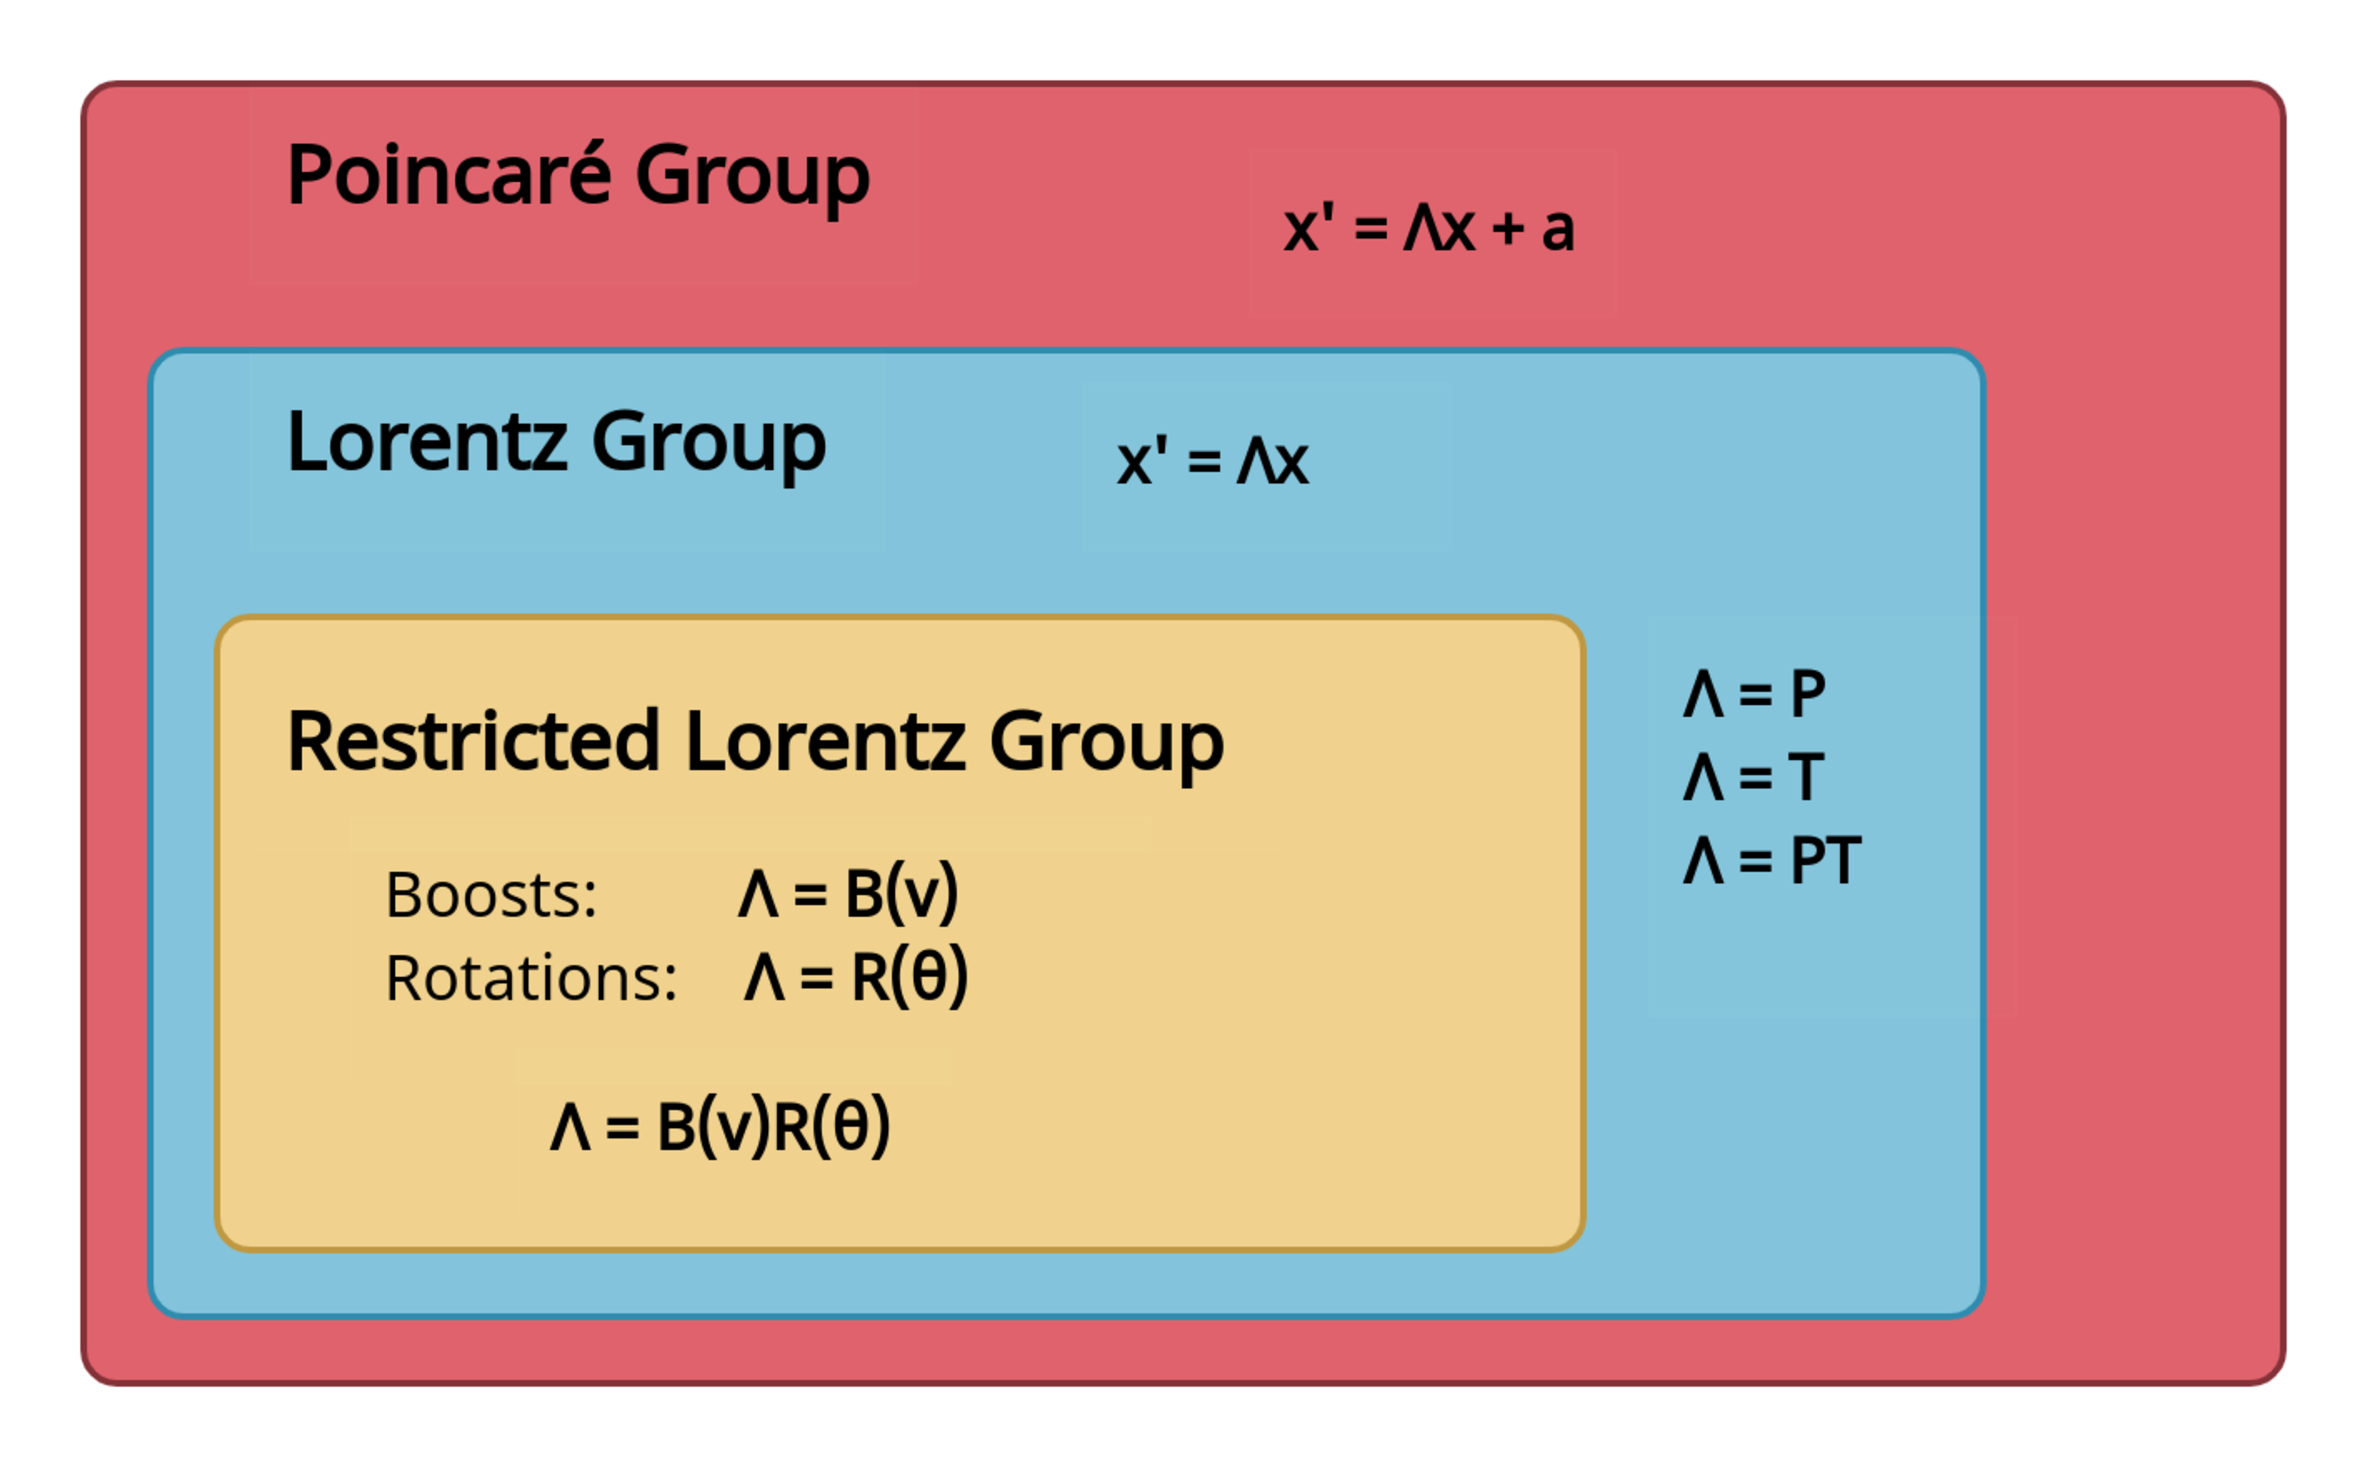
\includegraphics[width=.7\textwidth]{../Figuras/grupo-poincare.eps}
  \captionsetup{font=footnotesize, margin=8pt}
  \caption{Venn diagram of the Poincaré group and some of its subgroups. The Lorentz group elements P, T, and PT are the discrete transformations which take the identity component of the Lorentz group (i.e. the Restricted Lorentz Group) into the other three topologically separate components. Elements of the Restricted Lorentz Group include pure boosts, pure rotations, and general combinations of the two.}
  \label{poincare-subgroups}
\end{figure}
%

\section{Restricted Lorentz Group}

The subgroup of Lorentz transformations with $\det(\Lambda) = +1$ and $\Lambda^0_0 \geqslant +1$ is particularly important because it contains the identity, so that all of its elements can be connected to the identity by a continuous change of parameters, which ultimately means that all transformations have an infinitesimal form. Physically, these transformations correspond to spatial rotations and Lorentz boosts (transformations to a frame moving with uniform velocity). In a general four-dimensional setting, boosts and spatial rotations are actually unified: spatial rotations are simply rotations about a plane defined by two spatial axes, while boosts are hyperbolic rotations about a plane which includes the time axis. We mentioned before that the Lorentz group was six-dimensional: these six dimensions correspond to three rotation parameters (angles around three spatial axes) and three velocities (more precisely, {\it rapidities}) for boosts in each spatial direction.

To make things more concrete, let us look at the four-dimensional matrices $\Lambda$ for different transformations belonging to the proper orthochronous Lorentz group. First, a general Lorentz boost to a frame moving with velocity $\vb{v} = (v_x,v_y,v_z)$ is given by the matrix

\eq{ \label{general-boost-matrix} B(\vb{v}) = \begin{pmatrix}
\gamma & -\gamma \frac{v_x}{c} & -\gamma \frac{v_y}{c} & -\gamma \frac{v_z}{c} \\
-\gamma \frac{v_x}{c} & 1 + (\gamma - 1) \frac{v_x^2}{v^2} & (\gamma-1)\frac{v_x v_y}{v^2} & (\gamma-1)\frac{v_x v_z}{v^2} \\
-\gamma \frac{v_y}{c} & (\gamma-1)\frac{v_y v_x}{v^2} & 1 + (\gamma - 1) \frac{v_y^2}{v^2} & (\gamma-1)\frac{v_z v_y}{v^2} \\
-\gamma \frac{v_z}{c} & (\gamma-1)\frac{v_z v_x}{v^2} & (\gamma-1)\frac{v_y v_z}{v^2} & 1 + (\gamma - 1) \frac{v_z^2}{v^2} 
\end{pmatrix} ,
}
where $\gamma = (1 - (\frac{v}{c})^2)^{-1/2}$ is the Lorentz gamma factor. Perhaps more insight can be gained by looking at a boost in a particular direction. Conventionally, one considers boosts in the x direction (any boost can be made equal to this case through an appropriate choice of coordinate axes). Making $v_y = v_z = 0$ in \eqref{general-boost-matrix} we get
%
\eq{\label{x-boost-matrix} B(v\vu{x}) = \begin{pmatrix} \gamma & -\beta \gamma & 0 & 0 \\
-\beta\gamma & \gamma & 0 & 0 \\
0 & 0 & 1 & 0 \\
0 & 0 & 0 & 1 \end{pmatrix} ,
}
%
where $\beta = v/c$. Recall that the ordering we are using for the rows and columns is $(0, 1, 2, 3)$, so that the boost matrix above has the effect of ``mixing" the time coordinate with the spatial coordinate corresponding to the boost direction, while the other spatial directions (orthogonal to the boost direction) are left unchanged. 

An alternative parametrization in terms of the {\it rapidity} $\chi$ is often useful. Defining
%
\eq{ \chi \equiv \arctanh{\beta},
}
%
the Lorentz factor is then written as $\gamma = \cosh{\chi}$, and $\beta\gamma = \sinh{\chi}$. This ``coordinate change" maps the $-1<\beta<1$ interval of velocities to the $-\infty < \chi < \infty$ interval of rapidity. The Lorentz boost matrix takes the simplified form
%
\eq{\label{boost}B_x(\chi) = \begin{pmatrix} \cosh{\chi} & -\sinh{\chi} & 0 & 0 \\
-\sinh{\chi} & \cosh{\chi} & 0 & 0 \\
0 & 0 & 1 & 0 \\
0 & 0 & 0 & 1 \end{pmatrix} .
}
%
Rapidity is useful because, unlike velocities, it is additive. If you perform a first Lorentz boost to a frame moving with velocity $v_1$ and then a second boost, in the same direction, to a frame moving with $v_2$ (relative to this intermediate frame), then the velocity of the last frame with respect to the first is $v_{21} \neq v_1 + v_2$, since this simple composition rule would allow for $v_{21} > c$ in some cases\footnote{The correct formula for composing relativistic velocities is shown in the next section, when we discuss the Thomas-Wigner rotation.}. It holds, however, that $\chi_{21} = \chi_1 + \chi_2$.

For rotations, the four-dimensional matrix leaves the time coordinate invariant, and we have

\eq{\label{so3-matrix}R = \begin{pmatrix} 1 & 0 \\
0 & \vb{R}(\vb*{\theta})
\end{pmatrix} ,
}
%
where $\vb{R}(\vb*{\theta})$ is a usual three-dimensional orthogonal rotation matrix. For example, a rotation around the x axis by an angle $\theta$ is given by
%
\eq{\label{rotation}R_x(\theta) = \begin{pmatrix} 1 & 0 & 0 & 0 \\
0 & 1 & 0 & 0 \\
0 & 0 & \cos\theta & -\sin\theta \\
0 & 0 & \sin\theta & \cos\theta
\end{pmatrix}.
}
%
Notice how all of the matrices corresponding to proper orthocronous Lorentz transformations can be made equal to the identity by a continuous change of their parameters; for the boost matrices that happens in the limit $v \rightarrow 0$, while for rotation matrices the pertinent limit is $\theta \rightarrow 0$. This connection to the identity is one of the defining properties of the proper orthocronous Lorentz group and will be exploited in one of the following sections, when we look for the Hilbert space operators corresponding to these Lorentz transformations. Another thing to notice is that not all transformations of the restricted Lorentz group are pure boosts or pure rotations, but the most general transformation can be expressed as a product of {\it some} boost and {\it some} rotation.

The matrices \eqref{so3-matrix} form a (reducible) representation of the group of 3D rotations, $SO(3)$. In other words, rotations form a subgroup of the restricted Lorentz group. This is easy to see: since all rotations belong to the restricted Lorentz group and leave the time coordinate invariant, the product of two such transformations must also be a restricted Lorentz transformation, and it must also leave the time coordinte invariant (i.e., it can only be a rotation). The same cannot be said about boosts. 
The fact that boosts by themselves do not form a subgroup leads us to an important consequence of special relativity that will be prevalent in the rest of this work, and discussed thoroughly in the next section: the Thomas-Wigner rotation.

\section{Thomas-Wigner Rotation}
\label{sec:twr}

The equation $B(\vb{v})B(\vb{u})=B(\vb{w})$ can only be solved when velocities $\vb{v}$ and $\vb{u}$ are collinear; in this case, $\vb{w}$ will also be collinear to $\vb{v}$ and $\vb{u}$, with magnitude given by the one-dimensional velocity composition formula:

\eq{ w = \frac{v + u}{1 + \frac{v u}{c^2}} .
}
%
When the two velocities are non-collinear, however, the composition of the two boosts cannot be made equal to a boost. Instead, the result must be a more general transformation of the restricted Lorentz group, which is a product of a boost and a rotation:

\eq{\label{boost-composition} B(\vb{v})B(\vb{u}) = B(\vb{w})R_{\vu{n}}(\Omega) .
}
%
The rotation $R_{\vu{n}}(\Omega)$ is the so called Thomas-Wigner rotation, or simply Wigner rotation \cite{thomas_1926, wigner_1939}. It is a well-known consequence of special relativity, described in various textbooks \cite{jackson_1975, goldstein_1980} and still a topic of active research and debate to this day \cite{mocanu_1992, visser_2011, rebilas_2013, yarman_2020}.
The calculation of the actual rotation matrix $R_{\vu{n}}(\Omega)$ (or equivalently, the angle and axis of rotation) is a lengthy process that requires excessive amounts of algebra, so we will spare the reader of the details. We can, however, lay out the steps of the calculation, as we will do below.

\begin{figure}[t]
  \centering
  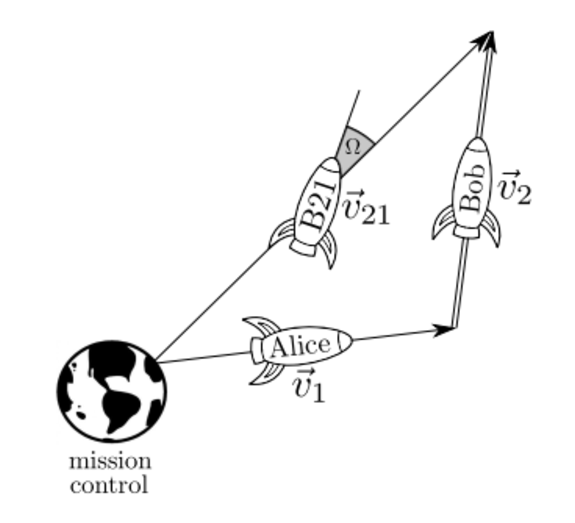
\includegraphics[scale=.6]{../Figuras/wig-rot-1.eps}
  \captionsetup{font=footnotesize, margin=8pt}
  \caption{Visualization of the Wigner rotation. Alice's ship is traveling with velocity $\vec{v}_1$ with respect to mission control, and Bob's ship is traveling with velocity $\vec{v}_2$ with respect to Alice's ship. Mission control sees Bob's ship traveling with velocity $\vec{v}_{21}$ and rotated by an angle $\Omega$. Figure taken from \cite{visser_2011}.}
  \label{alice-bob-rotation}
\end{figure}

Multiplying equation \eqref{boost-composition} by $B^{-1}(\vb{w})$ from the left, we get $R_{\vu{n}}(\Omega) = B^{-1}(\vb{w})B(\vb{v})B(\vb{u})$. The velocity $\vb{w}$ is the relativistic sum of velocities $\vb{v}$ and $\vb{u}$, obtainable through the general formula

\eq{\vb{w} = \frac{1}{1-\frac{\vb{u}\cdot\vb{v}}{c^2}}\left[ \frac{\vb{u}}{\gamma_v} - \vb{v} + \frac{\gamma_v}{1+\gamma_v}\frac{\vb{u}\cdot\vb{v}}{c^2}\vb{v} \right] ,
}
%
where $\gamma_v$ is the Lorentz factor associated with velocity $\vb{v}$. Having written $\vb{w}$ in terms of $\vb{v}$ and $\vb{u}$, we can then multiply the three matrices $B^{-1}(\vb{w})B(\vb{v})B(\vb{u})$ (recall that $B^{-1}(\vb{w}) = B(-\vb{w})$) to obtain the Wigner rotation matrix. The extraction of the angle and axis of rotation from the matrix follows from standard theory of 3D rotations. The axis can be obtained by solving the eigenvalue equation $R_{\vu{n}}(\Omega)\vu{n} = \vu{n}$, and the angle is related to the trace of $R_{\vu{n}}(\Omega)$ via $\Tr(R_{\vu{n}}(\Omega)) = 2 + 2\cos\Omega$. This whole process is carried through on \cite{visser_2011}, along with other methods of derivation. The result for the angle $\Omega$ is

\eq{\label{omega} \cos\Omega = \frac{(\gamma_w+\gamma_v + \gamma_u + 1)^2}{(\gamma_v + 1)(\gamma_u + 1)(\gamma_w + 1)} - 1 ,
}
%
and the axis of rotation is mutually orthogonal to both velocities being composed, that is:

\eq{ \vu{n} = \frac{\vb{v}\times\vb{u}}{\left|\vb{v}\times\vb{u}\right|} .
}
%
In other words, the {\it plane} of rotation is the plane described by the two velocity vectors $\vb{v}$ and $\vb{u}$. This makes the Wigner rotation easy to visualize in a simple 2D setting (see figure \ref{alice-bob-rotation}). Additionally, when the two velocities being composed are perpendicular to one another, equation \eqref{omega} simplifies to

\eq{\label{omega-perp} \cos\Omega = \frac{(\gamma_1 + 1)(\gamma_2 + 1)}{\gamma_1 \gamma_2 + 1} - 1.
}
%
It turns out that most of the examples studied in this work will fall under this category (composition of perpendicular velocities), so equation \eqref{omega-perp} above will be of great utility.

The Wigner rotation has been deemed a physical paradox that defies all logic and intuition, comparable to the likes of the twin paradox \cite{goldstein_1980}. In case the reader has not had this impression, we can frame it in a simpler but more dramatic manner: Alice's coordinate axes are parallel to both the mission control's axes and to Bob's axes; however, Bob's axes are {\it not} parallel to mission control axes. Notice that this rotation is ``static" (not a dynamical effect), resulting only from the kinematic relation between the three frames involved. When a particle's acceleration is non-parallel to it's velocity (for example, an electron orbiting a nucleus), the continuous composition of infinitesimal Wigner rotations gives rise to the Thomas precession, which in turn is a dynamical effect. While the Thomas precession plays an important role in the spin-orbit coupling and is essential to account for the fine-structure of atomic spectra, accelerated particles are outside of the scope of our investigations, and thus we shall limit our analysis to the static Wigner rotation only.

At this point, we have covered all of the special relativity concepts that will be important for the rest of the work. It may not yet be clear the role played by the Wigner rotation in QM to produce the peculiar entangling effect that is the centerpiece of the work. Pushing towards that understanding, we will now move on to discuss the standard methods of applying the principles of special relativity to QM, in a review mostly based upon ref. \cite{weinberg}.


\section{Relativistic Quantum Mechanics}
\label{rqm}

In QM, relativistic invariance requires that all Lorentz transformations have a corresponding unitary operator in the Hilbert space of states, i.e. the Hilbert space must carry a unitary representation of the Poincaré group. To see this, suppose that a Lorentz transformation $\Lambda$ takes the state $\ket{\alpha}$ into $\ket{\alpha'}$, and $\ket{\beta}$ into $\ket{\beta'}$. Relativistic invariance requires that both observers agree on the probabilities of transition between these states, which means that
%
\eq{\label{probab-invar} \left|\bra{\alpha}\ket{\beta}\right|^2 = \left|\bra{\alpha'}\ket{\beta'}\right|^2 ,
}
%
which can only be satisfied if the primed and unprimed states are related by
%
\eq{\begin{split}
\ket{\alpha'} &= U(\Lambda)\ket{\alpha}, \\
\ket{\beta'} &= U(\Lambda)\ket{\beta},
\end{split}
}
%
with $U(\Lambda)$ being unitary: $U^{-1} = U^\dagger$. In addition to unitarity, these operators must satisfy the group composition rule
%
\eq{U(\Lambda_1)U(\Lambda_2) = U(\Lambda_1\Lambda_2),
}
%
and $U(\Unit) = \Unit$ (the identity Lorentz transformation should correspond to the identity of the Hilbert space). As a consequence of these last two, we must also have $U(\Lambda^{-1}) = U^{-1}(\Lambda)$, since
%
\eq{ U(\Lambda)U(\Lambda^{-1}) = U(\Lambda\Lambda^{-1}) = U(\Unit) = \Unit .
}
%

\subsection{Unitary representations of the Poincaré group}

We will now follow the common procedure found in the literature of constructing the unitary operators from the infinitesimal form of the transformations. We start with pure translations (non-homogeneous transformations), since they are slightly simpler and the results look more familiar than the pure Lorentz transformations.

An infinitesimal translation is a coordinate transformation of the form

\eq{ x'^\mu = x^\mu + \epsilon^\mu,
}
%
with $\epsilon^\mu$ an infinitesimal four-vector. Since this transformation is infinitesimally close to the identity, the same should be true for the corresponding Hilbert space operator $U(\epsilon^\mu)$. Keeping only first order terms in $\epsilon^\mu$, we should have

\eq{ U(\epsilon^\mu) = \Unit - \frac{\epsilon_\mu \tilde{P}^\mu}{\hbar}.
}
%
For $U$ to be unitary, we must have

\eq{  U(\epsilon^\mu)U^\dagger(\epsilon^\mu) &= \left(\Unit - \frac{\epsilon_\mu \tilde{P}^\mu}{\hbar} \right) \left(\Unit - \frac{\epsilon_\mu \tilde{P}^{\mu\dagger}}{\hbar}\right) \nonumber \\
&= \Unit - \frac{\epsilon_\mu}{\hbar^2} ( \tilde{P}^\mu + \tilde{P}^{\mu\dagger} ) + O(\epsilon^2) \nonumber \\
&= \Unit ,
}
%
from which we get the requirement of anti-hermiticity for $\tilde{P}^\mu$: $\tilde{P}^{\mu\dagger} = -\tilde{P}^\mu$. It is actually convenient to define $P^\mu = -i\tilde{P}^\mu$, so that the infinitesimal transformation is written as

\eq{ \label{inf-trans} U(\epsilon^\mu) = \Unit - i\frac{\epsilon_\mu P^\mu}{\hbar},
}
%
and the requirement of anti-hermiticity for $\tilde{P}^\mu$ turns into a requirement of hermiticity for $P^\mu$: $P^{\mu\dagger} = P^\mu$. Extending \eqref{inf-trans} to a finite transformation is straightforward. By considering the composition of $N$ infinitesimal transformations, each with parameters $\epsilon_\mu = a_\mu/N$, and taking the limit $N \rightarrow \infty$,

\eq{U(a^\mu) &= \lim_{N \to \infty} \left( \Unit - i\frac{a_\mu P^{\mu}}{\hbar N} \right)^N \nonumber \\
&= e^{-i a_\mu P^\mu / \hbar}. \label{U-exp}
}
%
where $a^\mu = (c\Delta t, \Delta \vb{r})$ are the finite translation parameters.
Notice the resemblance to the non-relativistic time-translation and space-translation operators seen in chapter \ref{chap:qm}. In fact, the operator above can be seen as nothing more than a unification of both of these cases. The Hermitian four-vector operator $P^\mu$ has the connotation of being the generator of space-time translations, which allows us to identify it as the four-momentum observable.


A similar process can be used to obtain the unitary representation of pure Loretnz transformations, that is, coordinate transformations of the form

\eq{ x'^\mu = \Lambda^\mu_\nu x^\nu.
}
%
Since the identity transformation is $\Lambda^\mu_\nu = \delta^\mu_\nu$, an infinitesimal homogeneous Lorentz transformation should be
%
\eq{ \Lambda^\mu_\nu = \delta^\mu_\nu + \omega^\mu_\nu ,
}
%
with $\omega^\mu_\nu$ infinitesimal. For \eqref{lambda-invariance} to be satisfied, $\omega^\mu_\nu$ has to be antisymmetric: $\omega_{\mu\nu} = - \omega_{\nu\mu}$. By the same argument as before, the Hilbert space operator representing this transformation should look something like
%
\eq{\label{infinitesimalU} U(\delta^\mu_\nu + \omega^\mu_\nu) = \Unit + \frac{i}{2}\frac{\omega_{\mu\nu}J^{\mu\nu}}{\hbar} ,
}
%
where the imaginary unit was factored out in advancement of the anti-hermiticity requirement, and the factor of $1/2$ compensates for repeated terms in the sum ($\omega_{\mu\nu}J^{\mu\nu} =  \omega_{01}J^{01} + \omega_{10}J^{10} + ...$). The tensor operator $J^{\mu\nu}$ is also antisymmetric in its indices and must be Hermitian to guarantee the unitarity of $U$. Both $\omega_{\mu\nu}$ and $J_{\mu\nu}$, being 4x4 antisymmetric tensors, have six independent components. The three parameters $\omega_{0 i} = - \omega_{i 0} = \chi_i$ are the boost parameters (one for each direction), and the corresponding generators $J_{0 i} = - J_{i 0} = K_i$ are called the {\it boost generators}. The other three parameters $\omega_{i j} = -\omega_{j i} = \theta_k$ ($i,j,k$ cyclic) are the rotation parameters (one for each axis of rotation), and the corresponding generators $J_{i j} = -J_{j i} = J_k$ are the components of angular momentum. The entire tensor $J^{\mu\nu}$, which unifies boost and rotation generators, is commonly referred to as the relativistic angular momentum. Following the same procedure used for translations to obtain the finite extension of the infinitesimal operator, we get
%
\eq{U(\Lambda^\mu_\nu) = \exp(\frac{i}{2}\frac{\omega_{\mu\nu}J^{\mu\nu}}{\hbar}). 
}


\subsection{Four-momentum eigenstates}
\label{four-momentum-eigenstates}

Given the important role of the four-momentum operator as the Hermitian generator of space-time translations, it is convenient to use its eigenbasis to define states of a single particle. 
In the standard treatment of relativistic QM \cite{weinberg}, the single particle Hilbert space is spanned by states $\ket{p^\mu,\sigma}$ satisfying
%
\eq{\label{p-eigen} P^\mu \ket{p^\mu, \sigma} = p^\mu \ket{p^\mu, \sigma} ,
}
%
where $\sigma$ labels an additional discrete degree of freedom, taken here to be the value of a spin component. Equation \eqref{p-eigen} implies a simple transformation law under space-time translations. For a translation by a four-vector $a^\mu$, the corresponding unitary transformation on the basis states is
%
\eq{\label{Utranslation} U(a^\mu)\ket{p^\mu,\sigma} = \exp(-i\frac{p^\mu a_\mu}{\hbar})\ket{p^\mu, \sigma} .
}
%
While the transformation under translations is trivial when dealing with four-momentum eigenstates, the same is not true for pure Lorentz transformations. A subsequent section will be devoted to finding these transformation laws, and we will see that they involve the spin degree of freedom.

One momentum eigenstate which will be particularly important for our future purposes is the rest momentum state. For massive particles undergoing free evolution, there always exists a reference frame in which the particle is at rest; we denote the rest momentum as $k^\mu = (mc, \vec{0})$. Conversely, there always exists a set of Lorentz transformations $L(p)$ which take the rest momentum to any arbitrary momentum $p^\mu$:

\eq{ p^\mu = L(p)^\mu_\nu k^\nu .
}
%
The analogous statement in terms of states and operators of our Hilbert space is

\eq{\label{rest-frame} \ket{p^\mu, \sigma} =  U(L(p))\ket{k^\mu, \sigma}. 
}


\subsection{Mass-shell constraint}

In principle, any superposition of four-momentum eigenstates is a valid one particle state, which means a general state can be written as
%
\eq{\label{off-shell-state} \ket{\psi} = \sum_\sigma \int \dd[4]{p} \psi_\sigma(p^\mu) \ket{p^\mu,\sigma},
}
%
where $\psi_\sigma(p^\mu) \equiv \bra{p^\mu,\sigma}\ket{\psi}$ are the expansion coefficients. There is, however, an additional physical constraint that restricts the allowed states, which is that the norm of the momentum four-vector (a relativistic scalar) must be proportional to the rest mass of the particle:
%
\eq{ p^\mu p_\mu = \frac{E^2}{c^2} - \vb{p}^2 = m^2 c^2 ,
}
%
which is equivalent to requiring that the zeroth component of $p^\mu$ be $p^0 = E/c = \sqrt{\vb{p}^2+m^2c^2}$.
This so-called {\it mass-shell constraint} may be enforced directly in equation \eqref{off-shell-state} via
%
\eq{ \ket{\psi} = \sum_\sigma \int \dd[4]{p} \psi_\sigma(p^\mu) \delta(p^2 - m^2c^2) \theta(p^0) \ket{p^\mu,\sigma} ,
}
%
where $\delta(p^2 - m^2c^2)$ selects only mass-shell momenta and the Heaviside step function $\theta(p^0)$ selects only positive energy states. By integrating the $p^0$ component, one has
%
\eq{ \ket{\psi} &= \sum_\sigma \int \dd[3]{\vb{p}}\dd{p^0} \psi_\sigma(p^0, \vb{p}) \delta((p^0)^2 - \vb{p}^2 - m^2c^2) \theta(p^0) \ket{p^\mu,\sigma} \nonumber \\
&= \sum_\sigma \int \frac{\dd[3]{\vb{p}}}{2 \sqrt{\vb{p}^2 + m^2c^2}} \psi_\sigma(\sqrt{\vb{p}^2 + m^2c^2}, \vb{p})  \ket*{\sqrt{\vb{p}^2 + m^2c^2}, \vb{p},\sigma}.
}
%
This allows us to abandon the four-vector notation altogether, and rewrite the expression for a general state as
%
\eq{\label{shell-state} \ket{\psi} = \sum_\sigma \int \dd{\mu(\vb{p})} \psi_\sigma (\vb{p}) \ket{\vb{p}, \sigma},
}
%
where $\dd{\mu(\vb{p})} \equiv \dd[3]{\vb{p}}/2 \sqrt{\vb{p}^2 + m^2c^2}$ is the Lorentz-invariant mass-shell integration measure.
The corresponding orthonormality and completeness relations for the one particle Hilbert space, comprising only the states for which $p^0 = \sqrt{\vb{p}^2 + m^2c^2}$, are

\eq{\begin{split} \sum_\sigma \int \dd{\mu(\vb{p})} \dyad{\vb{p}, \sigma}  = \Unit , \\
\bra{\vb{p}, \sigma}\ket{\vb{p}', \sigma'} = 2p^0 \delta(\vb{p}-\vb{p}')\delta_{\sigma \sigma'} .
\end{split}
}
%
The expansion coefficients $\psi_\sigma(\vb{p})$, just like their non-relativistic counterparts, are to be interpreted as probability amplitudes in momentum representation, obeying the normalization requirement
%
\eq{ \sum_\sigma \int \dd{\mu(\vb{p})} |\psi_\sigma(\vb{p})|^2 = 1 .
}
%

\subsection{Transformation law for momentum and spin states}

The goal of this section is to determine how the momentum-spin states we have been considering so far transform under an arbitrary transformation $\Lambda$ of the restricted Lorentz group.

Using equation \eqref{rest-frame} to make reference to the particle's rest state, we have

\eq{U(\Lambda) \ket{\vb{p},\sigma} &=  U(\Lambda) U(L(\vb{p})) \ket{\vb{0},\sigma} \nonumber \\
&= U(\Lambda L(\vb{p})) \ket{\vb{0},\sigma} . \nonumber
}
%
From the discussions of section \ref{sec:twr}, the composition $\Lambda L(\vb{p})$ can be in general represented as a rotation followed by a boost, even when $\Lambda$ itself is a pure boost. To make this point explicit, we multiply the right hand side of the above equation by\footnote{The boldface $\vb*{\Lambda p}$ is to be understood as the spatial part of the four-vector $\Lambda^\mu_\nu p^\nu$.} $\Unit = U(L(\vb*{\Lambda p}))U^{-1}(L(\vb*{\Lambda p}))$:

\eq{ U(\Lambda) \ket{\vb{p},\sigma} &= U(L(\vb*{\Lambda p}))U^{-1}(L(\vb*{\Lambda p})) U(\Lambda L(\vb{p})) \ket{\vb{0},\sigma} \nonumber \\
&= U(L(\vb*{\Lambda p}))U(L^{-1}(\vb*{\Lambda p})\Lambda L(\vb{p})) \ket{\vb{0},\sigma} \nonumber \\
&= U(L(\vb*{\Lambda p}))U(W(\Lambda , p)) \ket{\vb{0},\sigma}. \nonumber
}
%
The transformation on the right hand side is a composition of a Wigner rotation $W(\Lambda, \vb{p}) \equiv L^{-1}(\vb*{\Lambda p})\Lambda L(\vb{p})$, which leaves the rest-momentum invariant (through the mapping $\vb{0} \rightarrow \vb{p} \rightarrow \vb*{\Lambda p} \rightarrow \vb{0}$), and a pure Lorentz boost $L(\vb*{\Lambda p})$ which, by definition, takes the rest momentum to $\vb*{\Lambda p}$. 

Since $U(W(\Lambda, \vb{p}))$ preserves the rest-momentum, it acts only on the internal (spin) degree of freedom. $U(W(\Lambda, \vb{p}))$ is then a $2s+1$ dimensional matrix which represents the group $SO(3)$ of spatial rotations. Denoting this matrix by $D(\Lambda, \vb{p})$ and acting with the pure boost $U(L(\vb*{\Lambda p}))$ in the rest-momentum, we finally get

\eq{\label{basis-transformation} U(\Lambda) \ket{\vb{p},\sigma} =  \sum_{\sigma'} D_{\sigma'\sigma}(\Lambda, \vb{p}) \ket{ \vb*{\Lambda p}, \sigma'} ,
}
%
where $D_{\sigma'\sigma}(\Lambda, \vb{p})$ represents an element of the Wigner rotation matrix, i.e. $D_{\sigma'\sigma}=\bra{\sigma'}D\ket{\sigma}$.
For spin-1/2 particles, $D(\Lambda, \vb{p})$ is the usual rotation matrix of a qubit:

\eq{\label{wig-rot-2x2} D(\Lambda, \vb{p}) = \cos(\frac{\Omega}{2}) + i \sin(\frac{\Omega}{2}) \vu{n}\cdot \vb*{\sigma} ,
}
%
with the angle $\Omega$ obtainable through equation \eqref{omega}, and the axis of rotation being mutually orthogonal to both velocities being composed; in this case, the particle momentum $\vb{p}$ and the boosted frame velocity $\vb{v}$:

\eq{\label{wig-rot-axis} \vu{n} = \frac{\vb{p}\times\vb{v}}{|\vb{p}\times\vb{v}|} .
}

Equation \eqref{omega} gives the angle $\Omega$ as a function of the velocities of the two boosts being composed. In the present case, one of these velocities is the velocity of the lab with respect to the particle's rest frame. The correspondence between the particle's momentum $\vb{p}$ and the velocity $\vb*{\beta}_1$ of the lab with respect to the particle is

\eq{ \vb*{\beta}_1 = - \frac{\vb{p}c}{E} = - \frac{\vb{p}}{p_0} ,
}
%
and the corresponding Lorentz $\gamma$ factor, in terms of the dynamical variables, is

\eq{ \label{gamma-dynamical} \gamma_1 = \frac{E}{mc^2} = \frac{p_0}{mc}.
}
%
Figure \ref{omega-x-beta} shows how the rotation angle $\Omega$ increases with the boost velocity, for different magnitudes of the momentum (which, for simplicity, is taken to be perpendicular to the boost direction).

\begin{figure}[t]
  \centering
  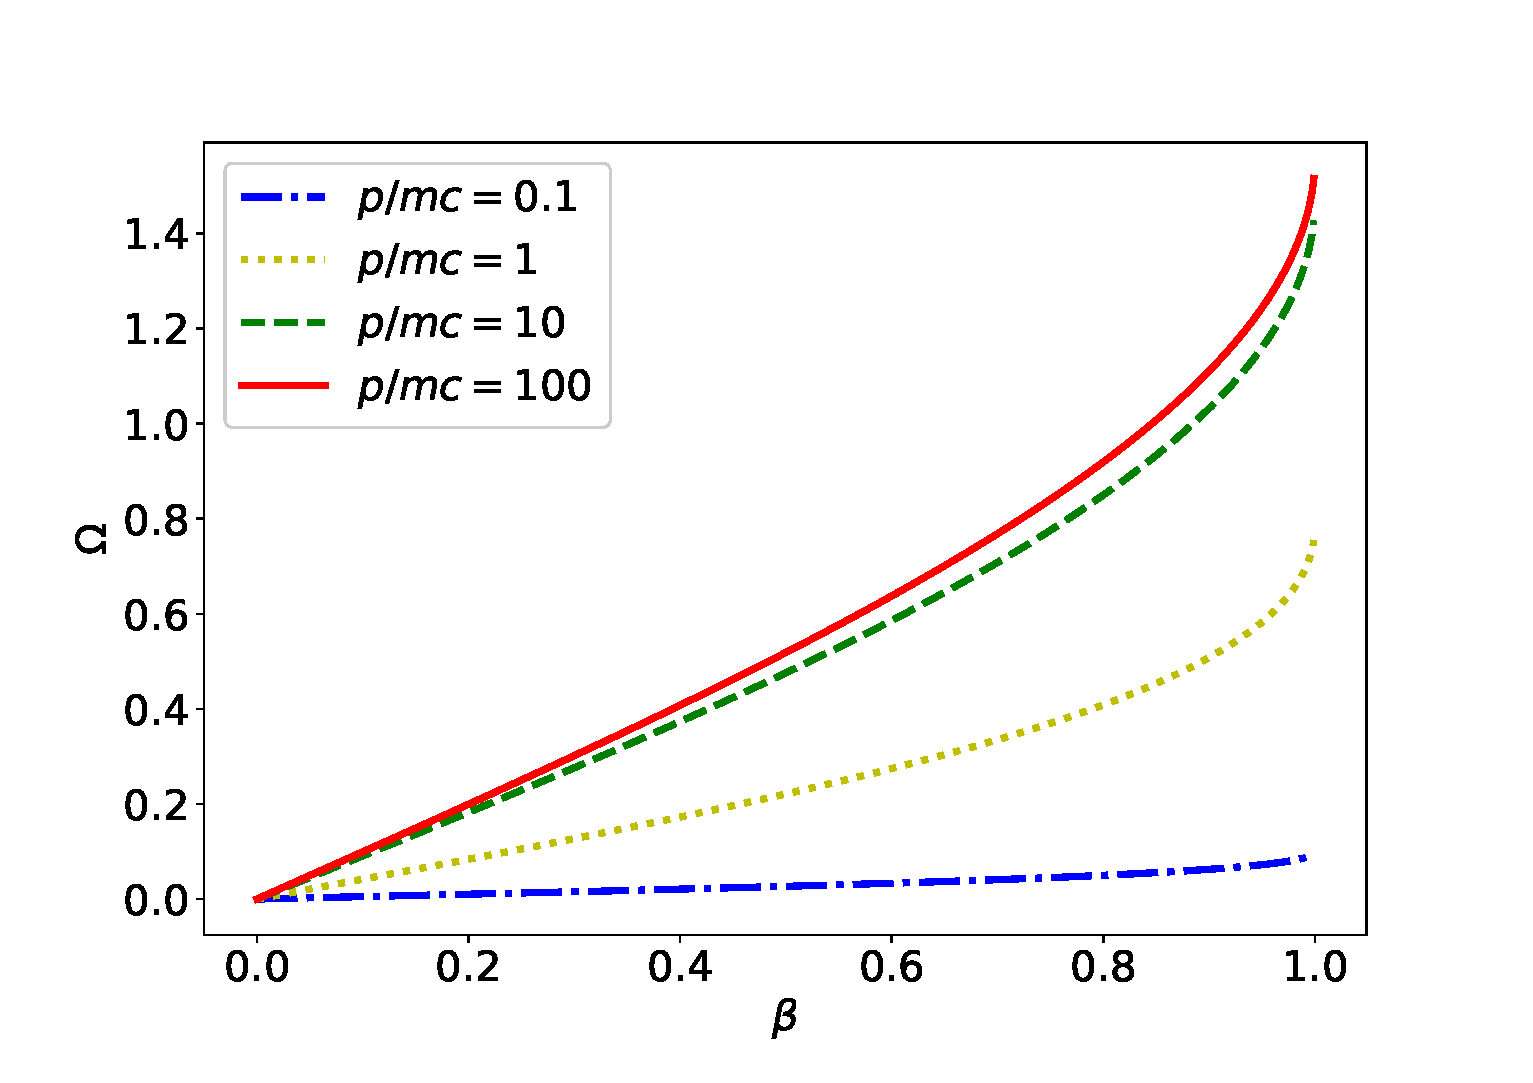
\includegraphics[width=.6\textwidth]{../Figuras/angulo.eps}
  \captionsetup{font=footnotesize, margin=8pt}
  \caption{Wigner rotation angle as a function of the boosted frame's velocity, for the case of a boost perpendicular to the particle's momentum. A particle with non-relativistic energy ($p/mc = 0.1$) results in negligible rotation, even for ultra-relativistic boosts ($\beta \rightarrow 1$). When the particle and the boost both approach ultra-relativistic velocities, the Wigner rotation angle approaches its maximal value of $\pi/2$.}
  \label{omega-x-beta}
\end{figure}

It is also possible to derive the $2\times2$ Wigner rotation matrix by multiplying the three Lorentz boosts that compose it. The $2\times2$ representation of a boost in the direction $\vu{e}$ with rapidity $\chi$ is given by

\eq{ K = \cosh\frac{\chi}{2} + \sinh\frac{\chi}{2} \vb*{\sigma}\cdot\vu{e},
}
%
while the boost that takes the rest momentum $k$ into an arbitraty momentum $p$ is

\eq{ C(p,k) = \left( \frac{p_0 + mc}{2mc} \right)^{1/2} + \left( \frac{p_0 - mc}{2mc} \right)^{1/2} \frac{\vb*{\sigma}\cdot\vb{p}}{|\vb{p}|}.
}
%
The Wigner rotation matrix can then be obtained through $D(\Lambda, \vb{p}) = C^{-1}(p',k) K C(p,k)$. The entire (very lengthy) calculation is done in \cite{halpern_1968}, and the result is

\eq{
\small
\label{wig-rot-2x2-alt} D(\Lambda, \vb{p}) = \frac{1}{\sqrt{(p_0 + mc)((\Lambda p)_0 + mc)}} \left\{ \cosh\frac{\chi}{2}(p_0 + mc) + \sinh\frac{\chi}{2}(\vb{p}\cdot\vu{e}) - i \sinh\frac{\chi}{2} \vb*{\sigma} \cdot (\vb{p}\times\vu{e}) \right\}.
\normalsize
}
%
The above form is completely equivalent to \eqref{wig-rot-2x2}; in fact they can be made equal through appropriate identification of the angle $\Omega$ and rotation axis $\vu{n}$. Both forms will be used in different parts of the work.


\pagebreak

\chapter{Boost-induced entanglement and irreality}

Now that we know how single particle basis states transform, and that the spin transformation is dependent on the value of the four-momentum, we are all set to understand how this leads to non-trivial consequences for entanglement and realism. We start off this chapter by considering a general scenario, making no assumptions about the system (other than being a free spin-1/2 particle). In the following sections we study two specific examples which were already investigated in the literature: a Gaussian wave-packet with well defined spin \cite{peres2002} and a particle in a superposition of two sharp, opposite momenta \cite{dunningham_palge_vedral_2009}. Lastly, we investigate the Mach-Zehnder interferometer, a system never before studied in a relativistic context.

\section{Transformation of general states}
\label{gen-states}

Knowing how the basis states transform under $\Lambda$ (equation \eqref{basis-transformation}), we can compute the transformation of any single particle state. Recalling the expression given in equation \eqref{shell-state} for a general state:

\eq{ \tag{\ref{shell-state}} \ket{\psi} = \sum_\sigma \int \dd{\mu(\vb{p})} \psi_\sigma (\vb{p}) \ket{\vb{p}, \sigma},
}
%
the corresponding boosted state $\ket{\psi'} = U(\Lambda)\ket{\psi}$ is given by

\eq{ \ket{\psi'} &= \sum_\sigma \int \dd{\mu(\vb{p})} \psi_\sigma (\vb{p}) U(\Lambda) \ket{\vb{p}, \sigma} \nonumber \\
&= \sum_\sigma \int \dd{\mu(\vb{p})} \psi_\sigma (\vb{p}) \sum_{\sigma'} D_{\sigma' \sigma}(\Lambda, \vb{p}) \ket{ \vb*{\Lambda p}, \sigma'} \label{gen-transf-state-0}, 
}
%
where we used \eqref{basis-transformation} to apply the transformation to the basis states. Denoting $\vb*{\pi} \equiv \vb*{\Lambda p}$, and using the Lorentz invariance of the integration measure, $\dd{\mu(\vb*{\pi})} = \dd{\mu(\vb{p})}$, we can put the above expression in the form of a general state similar to equation \eqref{shell-state}:

\eq{\label{gen-transf-state} \ket{\psi'} = \sum_{\sigma'} \int \dd{\mu(\vb*{\pi})} \phi_{\sigma'} (\vb*{\pi}) \ket{\vb*{\pi}, \sigma'} ,
}
%
where the transformed wave function $\phi_{\sigma'}(\vb*{\pi})$ is given by

\eq{\label{gen-transf-wf} \phi_{\sigma'}(\vb*{\pi}) \equiv \sum_\sigma D_{\sigma' \sigma}(\Lambda, \vb*{\Lambda^{-1}}\vb*{\pi}) \psi_\sigma (\vb*{\Lambda^{-1}}\vb*{\pi}) .
}
%
In matrix notation:

\eq{ \begin{bmatrix}[1.7] \phi_0(\vb*{\pi}) \\ \phi_1(\vb*{\pi}) \end{bmatrix} = \begin{bmatrix}[1.7] D_{00}(\Lambda, \vb*{\Lambda^{-1}}\vb*{\pi}) & D_{01}(\Lambda, \vb*{\Lambda^{-1}}\vb*{\pi}) \\ D_{10}(\Lambda, \vb*{\Lambda^{-1}}\vb*{\pi}) & D_{11}(\Lambda, \vb*{\Lambda^{-1}}\vb*{\pi}) \end{bmatrix} \begin{bmatrix}[1.7] \psi_0(\vb*{\Lambda^{-1}}\vb*{\pi}) \\ \psi_1(\vb*{\Lambda^{-1}}\vb*{\pi}) \end{bmatrix} .
\label{matrix-gen-transf}}
%
Thus we see that the effect of the boost on a general two component wave function is of rotating the ``internal" (spin) part of the wave function, while leaving the coordinate (momentum) part unchanged.

The fact that the Wigner rotation is a momentum dependent transformation on spin should be enough to notice that this transformation has the potential to create entanglement between the two degrees of freedom. In line with the discussions of section \ref{sec:entanglement}, the quantification of this sort of entanglement relies on determining the reduced density matrix and evaluating its entropy. The total density matrix associated with the state in \eqref{gen-transf-state} is

\eq{ \rho = \sum_{\sigma\sigma'}\int \dd{\mu(\vb{p})} \int \dd{\mu(\vb{q})} \phi_\sigma(\vb{p}) \phi^*_{\sigma'}(\vb{q}) \ket{\vb{p}, \sigma}\bra{\vb{q}, \sigma'} .
}
%
The spin reduced density matrix is given by
\eq{\rho_S &= \int \dd{\mu(\vb*{\pi})} \expval{\rho}{\vb*{\pi}} \nonumber \\
&= \sum_{\sigma\sigma'} \int \dd{\mu(\vb*{\pi})} \phi_\sigma(\vb*{\pi})\phi^*_{\sigma'}(\vb*{\pi}) \ket{\sigma}\bra{\sigma'} \nonumber \\
&= \begin{bmatrix}[1.7] \int |\phi_0(\vb*{\pi})|^2 \dd{\mu(\vb*{\pi})} & \int \phi_0(\vb*{\pi}) \phi_1^*(\vb*{\pi}) \dd{\mu(\vb*{\pi})} \\
\int \phi_1(\vb*{\pi}) \phi_0^*(\vb*{\pi}) \dd{\mu(\vb*{\pi})} & \int |\phi_0(\vb*{\pi})|^2 \dd{\mu(\vb*{\pi})}
\end{bmatrix}. \label{relativistic-sdm}
}
%
The reduced density matrix above was the main object of study in the seminal work of Peres et al. \cite{peres2002}. There, the main conclusion was that the spin reduced density matrix is not covariant under Lorentz transformations, and therefore the spin entropy (which usually quantifies entanglement) has ``no invariant meaning". In the next section we will take a closer look at those results.


An interesting question to ask is if this sort of entanglement can ``destroy" momentum coherence. We know that, if position or momentum become entangled with an external degree of freedom, this degree of freedom may act as an ``informer", storing information about the momentum, which has the effect of suppressing interference terms (off-diagonal terms) of the density matrix. It is a plausible hypothesis, then, that a boosted reference frame may verify the effects of spin-momentum entanglement through the observation of a different momentum probability density (i.e. a different interference pattern in a diffraction experiment). Given the state in \eqref{shell-state}, the probability of finding the particle with momentum $\vb{p}$ is given by the Born rule, using the infinitesimal projector $\dyad{\vb{p}}\dd{\mu(\vb{p})}$:

\eq{ \dd \mathfrak{p}(\vb{p}) &= \Tr\bigg[\big(\dyad{\vb{p}}\dd{\mu(\vb{p})}\otimes\Unit_S\big) \dyad{\psi}\bigg] \nonumber \\
&= \sum_\sigma |\psi_\sigma(\vb{p})|^2 \dd{\mu(\vb{p})} \nonumber \\
&= \psi^\dagger(\vb{p}) \psi(\vb{p}) \dd{\mu(\vb{p})} ,
\label{inf-prob}}
%
where $\psi(\vb{p})$ denotes the two-component column vector $\psi(\vb{p}) = (\psi_0(\vb{p}), \psi_1(\vb{p}))^T$. From the above, we identify the momentum probability density 

\eq{\Gamma(\vb{p}) := \frac{\dd \mathfrak{p}(\vb{p})}{\dd{\mu(\vb{p})}} = \psi^\dagger(\vb{p}) \psi(\vb{p}) .
}

To determine the probability density seen by the moving frame, we start with a similar expression as in \eqref{inf-prob}. The infinitesimal projector remains $\dyad{\vb{p}}\dd{\mu(\vb{p})}$, but we use the transformed state $\ket{\psi'}$ of \eqref{gen-transf-state-0}\footnote{This corresponds to the active picture. The same probability could be obtained by transforming the projector and using the original state $\ket{\psi}$.}. Following the same steps of equation \eqref{inf-prob}, we obtain an equivalent expression for the probability density seen by the moving frame:

\eq{ \Gamma'(\vb{p}) = \phi^\dagger(\vb{p}) \phi(\vb{p}).
}
Using equation \eqref{gen-transf-wf}, this becomes

\eq{\Gamma'(\vb{p}) &= \psi^\dagger(\vb*{\Lambda^{-1}}\vb{p})D^\dagger(\Lambda, \vb*{\Lambda^{-1}}\vb{p}) D(\Lambda, \vb*{\Lambda^{-1}}\vb{p})\psi(\vb*{\Lambda^{-1}}\vb{p}) \nonumber \\
&= \psi^\dagger(\vb*{\Lambda^{-1}}\vb{p})\psi(\vb*{\Lambda^{-1}}\vb{p}) \nonumber \\
&= \Gamma(\vb*{\Lambda^{-1}}\vb{p}),
}
%
where we see that, because of the unitarity of $D(\Lambda, \vb{p})$, the probability density remains the same in both frames. The type of entanglement induced by Lorentz boosts is thus shown to be ``non-decohering": it cannot affect the momentum probability density. This is in contrast to the usual type of ``decohering" entanglement, in which an external degree of freedom stores ``which-way" information about the particle, which in turn can affect the probability density (attenuating an interference pattern).

%In hindsight, the result couldn't have been different: if we recall the initial discussion of section \ref{rqm}, the requirement of unitarity was to ensure that the probabilities (which constitute the experimentally accessible results of quantum theory) remain the same in both frames, so as to not violate relativity. 

%This can be summarized as a statement about the difference between internal and external entanglement. Because momentum is entangled with an internal degree of freedom, no effect is observed in the momentum probability density due to this entanglement. This is in contrast to the usual type of ``decoherence" entanglement (which relies on an external degree of freedom storing ``which-way" information about the particle, which can then be reflected in the momentum probability density).

Another consequence of unitarity, interesting in the context of quantum information, is that $I(\rho) = I(U\rho U^\dagger)$: the amount of information contained in the total quantum state is the same for both reference frames. However, for the map of unrevealed measurements $\Phi_A(\rho)$, all that can be said is $\Phi_A(U\rho U^\dagger) = \Phi_{U^\dagger AU}(\rho)$, due to the equivalence between active picture (transformation applied to the state) and passive picture (inverse transformation applied to the observables). As noted in \cite{savi_angelo_2021}, none of these states are equal to $\Phi_A(\rho)$ or $U\Phi_A(\rho)U^\dagger$, implying that the information removed from a state by the map $\Phi_A(\rho)$ is not the same for two unitarily-connected Lorentz frames. This, in turn, implies the non-covariance of quantum coherence, $\mathbb{C}_A(\rho_\mathcal{A}) = S(\Phi_A(\rho_\mathcal{A})) - S(\rho_\mathcal{A})$, and irreality, $\mathfrak{I}_A(\rho) = S(\Phi_A(\rho)) - S(\rho)$. To gain further insight into how entanglement and irreality are affected by Lorentz transformations, we will now look into specific case studies.

\section{Gaussian state}

We will start by reviewing the result of Peres, Scudo and Terno \cite{peres2002}, from the seminal work that brought to light the entanglement effects of Lorentz transformations and its consequences to quantum information theory. They considered an initial state consisting of a Gaussian wave function, centered around the rest momentum $\vb{p}_0 = 0$, with spin pointing in the positive z direction:

\eq{ \psi_0(\vb{p}) = \frac{1}{(2\pi\Delta^2)^{3/4}} \exp\left(\frac{-\vb{p}^2}{2 \Delta^2}\right) ,
}
%
with $\psi_1(\vb{p}) = 0$. It is simple to see that this is a state for which the $\sigma_z$ component of spin is an element of reality.

They then proceeded to consider the same state seen from an observer moving with velocity $\beta$ in the positive x direction. They use the form of the Wigner rotation matrix given in equation \eqref{wig-rot-2x2-alt}, with boost direction $\vu{e} = \vu{x}$ and rapidity $\chi$, obtaining the transformed wave function

\eq{ \phi_0(\vb{p}) &= K \left[ C(p^0 + mc) + S(p_x + i p_y) \right] \psi_0(\vb*{\Lambda^{-1}}\vb{p}) , \\
\phi_1(\vb{p}) &=  KSp_z \psi_0(\vb*{\Lambda^{-1}}\vb{p}) ,
}
%
where $K = \left[(p^0 + mc)(p'^0 + mc)\right]^{-1/2}$, $C = \cosh\frac{\chi}{2}$ and $S = \sinh\frac{\chi}{2}$. The reduced density matrix was obtaind through \eqref{relativistic-sdm}, and its entropy was found to be

\eq{\label{peres-entropy} S(\rho_S) \approx t(1 - \ln t),
}
where $t = \tfrac{1}{8}(\tfrac{\Delta}{mc})^2 \tanh^2\frac{\chi}{2}$, and the approximation being considered is $\Delta <\!\!< mc$. Interesting points of analysis are that, for $\Delta \rightarrow 0$ we get a localized momentum state, and the entropy goes to zero, as expected. For $\chi = 0$ we recover the results of the original reference frame, for which the reduced spin state is pure (entropy also goes to zero). Equation \eqref{peres-entropy} implies that observers moving at different speeds (i.e., different rapidities $\chi$) will observe a different purity for the spin state; equivalently, different entanglement between spin and the only other degree of freedom (momentum). 

If we wish to investigate the degree of irreality (of spin and/or momentum) for the state in this example, we run into some problems; specifically, we would need to evaluate the von Neumann entropy of an infinite dimensional density matrix. This issue could be circumvented by using a discretization of the momentum space, as was shown in \cite{freire_angelo_2019}. The discretization of a Gaussian state would involve too many technical nuances, so we leave the discussions of realism to the next examples, for which the momentum discretization comes more naturally.

\section{Superposition of two opposite momentum eigenstates}
\label{opposite-momenta}

The next example is a slight adaptation and generalization of a model first studied in \cite{dunningham_palge_vedral_2009}, consisting of a single relativistic particle in a superposition of opposite propagating momentum states. For this system, in addition to quantifying the bipartite entanglement between spin and momentum (which was already done in \cite{dunningham_palge_vedral_2009}), we will address the main question of our work; namely, how a Lorentz boost affects the realism of spin and momentum.

We take the particle's propagation direction to be along the z axis, such that the two four-momenta being considered are $p_+ = (E_p/c,0,0,p)$ and $p_- = (E_p/c, 0, 0, -p)$, where $E_p = \sqrt{p^2c^2 + m^2c^4}$. The state of the particle, seen from the laboratory frame $\mathcal{S}$, is

\eq{\label{opposite-momenta-state}\ket{\psi} = \frac{\ket{p_+}+\ket{p_-}}{\sqrt{2}}\otimes \ket{\Phi} ,
}
%
with $\ket{\Phi} = \cos\frac{\theta}{2}\ket{0} + e^{i\phi}\sin\frac{\theta}{2}\ket{1}$ a general spin state in the Bloch representation. Since this model concerns two sharp momentum states, the momentum degree of freedom can be effectively treated as a qubit, with $\ket{p_+}$ and $\ket{p_-}$ forming the effective orthonormal basis of the Hilbert space. In appendix \ref{app-a} we discuss how this discretization of the momentum space can be made rigorous through the use of Dirac delta distributions in the  wave function.

Next we will consider the same system as seen from a reference frame $\mathcal{S}'$ moving with constant velocity in a direction perpendicular to the z axis. This can be taken to be the x axis without loss of generality, since the only feature of the system that breaks azimuthal symmetry is the spin, whose components in the x and y directions are dictated by the angle $\phi$. Varying the boost direction in the x-y plane would then be equivalent to varying the spin azimuthal angle $\phi$, so by fixing the boost velocity $\vb{v} = \beta c \vu{x}$ in the x direction we avoid the addition of a redundant parameter.

The effect of the Lorentz boost is given by \eqref{basis-transformation}:

\eq{\begin{split} U(\Lambda)\ket{p_+}\ket{\Phi} &= \ket{\Lambda p_+}D(\Lambda, p_+)\ket{\Phi}, \\
U(\Lambda)\ket{p_-}\ket{\Phi} &= \ket{\Lambda p_-}D(\Lambda, p_-)\ket{\Phi} .
\end{split}
}
%
The Wigner rotations $D(\Lambda, p_+)$ and $D(\Lambda, p_-)$ associated with opposite momenta are both rotations around the y axis by the same angle but in opposite directions, since $\vb{v} \times \vb{p_+} = - (\vb{v} \times \vb{p_-})$. Recall from section \ref{sec:twr} that when two perpendicular velocities are being composed, the angle of the Wigner rotation is given by equation \eqref{omega-perp}:

\eq{\tag{\ref{omega-perp}} \cos\Omega = \frac{(\gamma_1 + 1)(\gamma_2 + 1)}{\gamma_1 \gamma_2 + 1} - 1 ,
}
%
where in this case $\gamma_2 \equiv \gamma_\Lambda$ is the Lorentz factor associated with the boost $\Lambda$, and $\gamma_1 = E_p/mc^2$ is the Lorentz factor associated with the boost to the particle's rest frame. Plugging all this in and doing some algebra, we get a neat formula for the angle:

\eq{\label{omega-neat} \cos\Omega = \frac{E_p + \gamma_\Lambda m c^2}{\gamma_\Lambda E_p + m c^2}.
}
%

The state $\ket{\psi'} = U(\Lambda)\ket{\psi}$ seen from the $\mathcal{S}'$ frame is

\eq{ \ket{\psi'} = \frac{\ket{\Lambda p_+}D(\Lambda, p_+)\ket{\Phi} + \ket{\Lambda p_-}D(\Lambda, p_-)\ket{\Phi}}{\sqrt{2}},
}
%
from which we can already see the same intriguing fenomenon from the last example: while in the original frame, spin and momentum factorize, in the moving frame there can be spin-momentum entanglement. In this discretized example, the partial trace takes the simplified form

\eq{ \rho'_S = \Tr_p(\rho') = \mel{\Lambda p_+}{\rho'}{\Lambda p_+} + \mel{\Lambda p_-}{\rho'}{\Lambda p_-} ,
}
%
with $\rho' = \dyad{\psi'}$. The resulting spin reduced density matrix is

\eq{\label{sdm-example2} \rho'_S \stackrel{\cdot}{=} \begin{bmatrix}[1.7] \cos^2\frac{\Omega}{2}+\sin^2\theta\sin^2\phi\sin^2\frac{\Omega}{2} & -\sin\theta\sin\phi(\cos\theta\sin\phi-i\cos\phi)\sin^2\frac{\Omega}{2} \\ -\sin\theta\sin\phi(\cos\theta\sin\phi+i\cos\phi)\sin^2\frac{\Omega}{2} & (\cos^2\phi + \cos^2\theta\sin^2\phi)\sin^2\frac{\Omega}{2} \end{bmatrix} .
}
%
To clear things out, let's consider specific spin directions for the initial state $\ket{\Phi}$. When $\theta \in \{0, \pi\}$ we have a $\sigma_z$ eigenstate ($\ket{\Phi} = \ket{0}$ or $\ket{\Phi} = \ket{1}$). When $\theta = \frac{\pi}{2}$ and $\phi \in \{0, \pi\}$, we have a $\sigma_x$ eigenstate ($\ket{\Phi} = \ket{+}$ or $\ket{\Phi} = \ket{-}$). In both of these cases (spin in the z or x direction), \eqref{sdm-example2} simplifies to

\eq{ \rho'_S = \begin{bmatrix} \cos^2\frac{\Omega}{2} & 0 \\ 
0 & \sin^2\frac{\Omega}{2} \end{bmatrix}.
}
%
With the two simple eigenvalues $\cos^2\frac{\Omega}{2}$ and $\sin^2\frac{\Omega}{2}$, the entropy of entanglement takes the form

\eq{ S(\rho'_S) &= h\left(\cos^2\frac{\Omega}{2}\right) \nonumber \\
&= -\cos^2\frac{\Omega}{2} \log_2\left(\cos^2\frac{\Omega}{2}\right) -  \sin^2\frac{\Omega}{2}\log_2 \left(\sin^2\frac{\Omega}{2}\right).
}
%
Recall that the angle $\Omega$ is actually a (monotonically increasing) function of the boost velocity. Figure \ref{entanglement-counter} shows a plot of the entropy of entanglement as a function of the dimensionless velocity $\beta$ of the moving frame. For $\beta = 0$, we retain the original frame of reference, for which the state is separable and thus the entanglement is zero. For increasing boost velocities, the entanglement increases monotonically, with a steep increase when $\beta \rightarrow 1$ (reflective of the way $\Omega$ increases with $\beta$, see figure \ref{omega-x-beta}).

\begin{figure}[t]
  \centering
  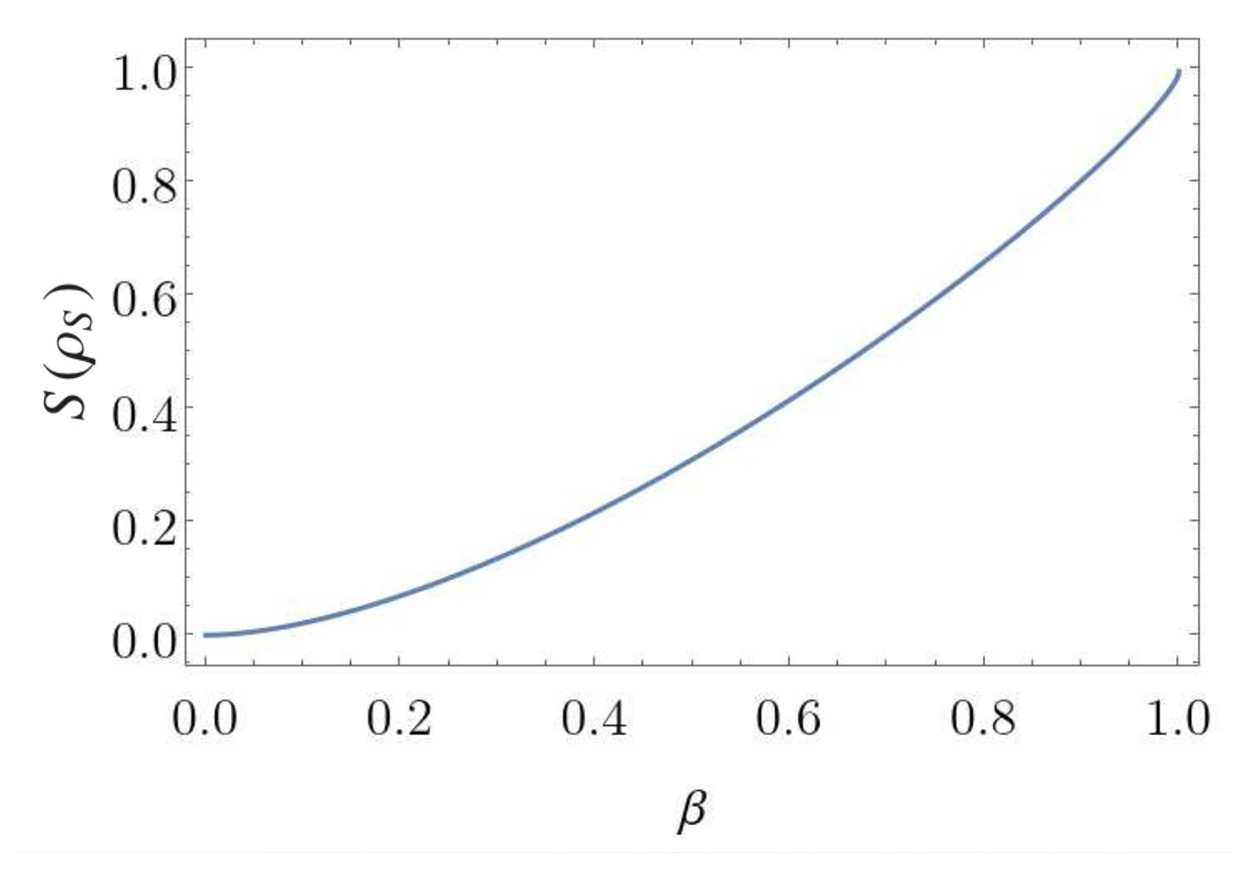
\includegraphics[scale=.42]{../Figuras/entanglement-counter.eps}
  \captionsetup{font=footnotesize, margin=8pt}
  \caption{Entropy of entanglement (von Neumann entropy of the reduced density matrix), measured in bits, of the state $\ket{\psi'}$ as a function of the adimensional boost velocity $\beta$.}
  \label{entanglement-counter}
\end{figure}

If, on the other hand, the spin is initially a $\sigma_y$ eigenstate ($\theta=\frac{\pi}{2}$ and $\phi \in \{\frac{\pi}{2}, \frac{3\pi}{2}\}$), the reduced density matrix \eqref{sdm-example2} simplifies to

\eq{\rho'_S \stackrel{\cdot}{=} \begin{bmatrix} 1 & 0 \\ 
0 & 0 \end{bmatrix} ,
}
%
or simply $\rho'_S = \dyad{\Phi}$. This is pure for any boost velocity, indicating that spin and momentum remain separate in this particular case. The reason for the lack of entanglement is straightforward: in this particular geometric configuration (particle in the z axis, boost in the x axis) the Wigner rotation is around the y axis, and thus if the spin is initially along the y direction, it remains unaffected by the boost.

\subsection{Relativity of reality}

Within this case study, we will now investigate a fundamental question: is reality absolute or relative? Do all observers agree about whether or not a physical quantity is an element of reality? Since the quantum correlations show an interesting and non-trivial behavior in the relativistic setting, we expect to see an equally interesting behavior regarding the realism of the degrees of freedom concerned. To tackle this question, we will use BA's realism framework presented in section \ref{ba} to assess how the reality status of spin and momentum change when the Lorentz boost is applied.

The general spin state $\ket{\Phi}$ considered so far is an eigenstate of the spin component in the general direction $\vu{n} = (\sin\theta\cos\phi, \sin\theta\sin\phi, \cos\theta)$, which means that $\sigma_{\vu{n}} \ket{\Phi} = \ket{\Phi}$. We will denote the other eigenstate, associated with the negative eigenvalue, by $\ket{\Phi_\bot}$ (in the $\sigma_z$ basis: $\ket{\Phi_\bot} = \sin\frac{\theta}{2}\ket{0} - e^{i\phi}\cos\frac{\theta}{2}\ket{1}$), such that the $\vu{n}$-component of spin has spectral decomposition $\sigma_{\vu{n}} = \dyad{\Phi} - \dyad{\Phi_\bot}$. To calculate the irreality of $\sigma_{\vu{n}}$ for a state $\rho$, we apply the map of unrevealed measurements

\eq{\label{spin-map} \Phi_{\sigma_{\vu{n}}}(\rho) = \dyad{\Phi} \rho \dyad{\Phi} + \dyad{\Phi_\bot} \rho \dyad{\Phi_\bot}.
}
%

The first thing to notice is that, for the state \eqref{opposite-momenta-state} seen by the lab frame, $\sigma_{\vu{n}}$ is an element of reality:

\eq{ \rho = \Phi_{\sigma_{\vu{n}}}(\rho)
}
%
for $\rho = \dyad{\psi}$. This should come as no surprise, since we are explicitly choosing a spin observable for which the spin state is an eigenstate. Spin is here an element of reality under EPR's criterion as well: we don't need to disturb the system in any way to predict that a measurement of $\sigma_{\vu{n}}$ will yield a spin up result 100\% of the time.

To assess the reality status of spin for the moving frame $\mathcal{S}'$, we substitute the transformed state $\rho' = \dyad{\psi'}$ into \eqref{spin-map}. Since $\rho'$ is pure, $S(\rho') = 0$, and the irreality $\mathfrak{I}_{\sigma_{\vu{n}}}(\rho')$ is simply the von Neumann entropy of  $\Phi_{\sigma_{\vu{n}}}(\rho')$. In terms of the binary entropy $h(x)$ (equation \eqref{binary}), the irreality is

\eq{ \mathfrak{I}_{\sigma_{\vu{n}}}(\rho') = h\Bigg(\frac{1}{4}\big(3+\cos 2\theta + 2\cos 2\phi\ \sin^2\theta\big)\sin^2\frac{\Omega}{2}\Bigg).
}
%
This is symmetrical under the exchange $\theta \leftrightarrow \phi$, a fact which is not obvious by inspection of the expression, but which can be partially verified (for the cases when $\theta = \frac{\pi}{2}$ and $\phi = \frac{\pi}{2}$) in figure \ref{spin-irreality-counter}, in which $\mathfrak{I}_{\sigma_{\vu{n}}}(\rho')$ is plotted as a function of the boost velocity $\beta$ and the angles $\theta$ and $\phi$.

\begin{figure}[t]
  \centering
  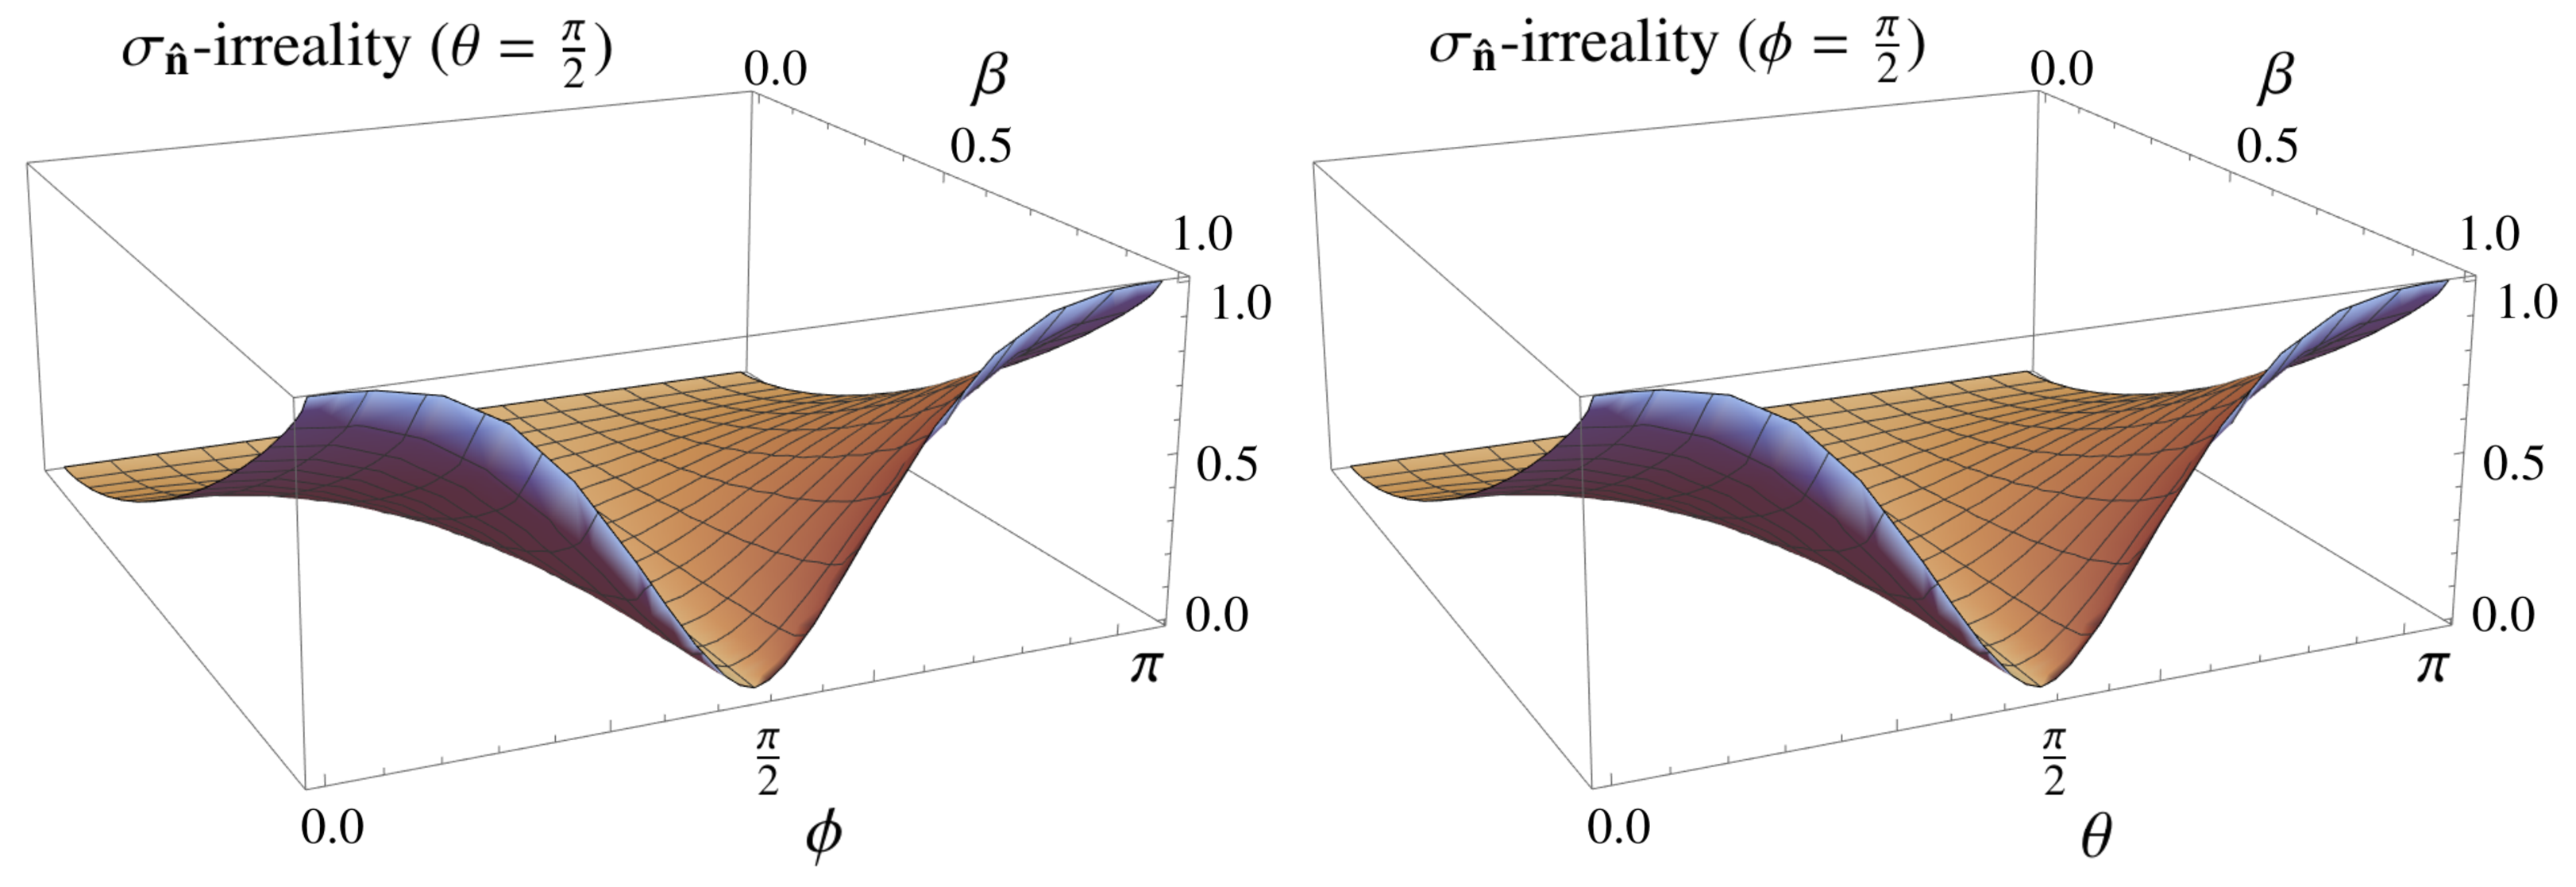
\includegraphics[scale=.3]{../Figuras/improved/spin-irreality-counter-IMPROVED.eps}
  \captionsetup{font=footnotesize, margin=8pt}
  \caption{Irreality of the $\vu{n}$ component of spin for the particle in a superposition of counter-propagating momenta (state given in equation \eqref{opposite-momenta-state}). On the left, the initial spin state is in the equator of the Bloch sphere ($\theta = \tfrac{\pi}{2}$), and $\mathfrak{I}_{\sigma_{\vu{n}}}(\rho')$ is plotted as function of the boost velocity $\beta$ and the azimuthal angle $\phi$. On the right, the spin is in the meridian $\phi = \tfrac{\pi}{2}$ of the Bloch sphere, and $\mathfrak{I}_{\sigma_{\vu{n}}}(\rho')$ is shown as function of the boost velocity $\beta$ and the polar angle $\theta$.}
  \label{spin-irreality-counter}
\end{figure}

Just like we did for entanglement, we will ``clear up" this result by considering particular spin directions. When the spin is in the y direction ($\theta = \frac{\pi}{2}$ and $\phi \in \{ \frac{\pi}{2}, \frac{3 \pi}{2}\}$), the expression above simplifies to $h(0) = 0$. This is the uninteresting case in which there is no entanglement seen from $\mathcal{S}'$, and also, as we verify now, no difference in the spin-reality. When the spin is either in the z or x direction, the irreality simplifies to $\mathfrak{I}_{\sigma_{\vu{n}}}(\rho) = h(\sin^2\tfrac{\Omega}{2}) = h(\cos^2\tfrac{\Omega}{2})$, which is exactly the same expression as the entropy of entanglement, whose behavior is depicted in figure \ref{entanglement-counter}. The fact that irreality is equal to entanglement can be better understood by computing the local irreality, or $\sigma_{\vu{n}}$ coherence:

\eq{ \mathbb{C}_{\sigma_{\vu{n}}}(\rho'_S) = S(\Phi_{\sigma_{\vu{n}}}(\rho'_S)) - S(\rho'_S).
}
%
We find that this is zero, not only for spin in the y direction but also in the x and z directions. Recalling that the total irreality can be decomposed into a local contribution (due to coherence) and a global contribution (due to quantum correlations), and noticing that in this case the former is zero, it becomes clear why the irreality is equal to entanglement.

The computation of the momentum irreality involves some technical subtleties. The boost maps the qubit basis $\{ \ket{p_+}, \ket{p_-} \}$ into $\{ \ket{\Lambda p_+}, \ket{\Lambda p_-} \}$, but there's no clear way to write the former states as a linear combination of the latter (we have effectively mapped one qubit Hilbert space into a different qubit space). To circumvent this apparent issue, we must go back to a more rigorous approach and consider that all four of these states belong to the same Hilbert space and are orthonormal to one another. Within our discretized treatment, this means we are dealing with a four-dimensional space. The map $\Phi_P(\rho)$ involves all four projectors, while the state $\rho$ in the lab frame only involves the states $\ket{p_+}$ and $\ket{p_-}$, while the state $\rho'$ in frame $\mathcal{S}'$ involves only $\ket{\Lambda p_+}$ and $\ket{\Lambda p_-}$. The post-measurement state in the lab frame is

\eq{ \Phi_P(\rho) = \frac{\dyad{p_+} + \dyad{p_-}}{2} \otimes \dyad{\Phi} ,
}
%
while in the boosted frame, it is

\eq{ \Phi_P(\rho') = \frac{\dyad{\Lambda p_+}\otimes D_+\dyad{\Phi}D_+^\dagger + \dyad{\Lambda p_-}\otimes D_-\dyad{\Phi}D_-^\dagger}{2}.
}
%
Notice that for both frames, the post-measurement state is a statistical mixture with probabilities $1/2$, meaning $S(\Phi_P(\rho)) = S(\Phi_P(\rho')) = h(1/2) = 1$. This makes it so that the total momentum irreality is boost-independent. What is not boost-independent, however, is how much of the irreality is due to local contributions (coherence) vs. non-local contributions (entanglement). Since entanglement was shown to increase with the boost velocity, there is a trade-off for the total irreality to remain constant: the moving frame sees a decrease in coherence, to compensate for the increase in quantum correlations.

By looking at this example we verify, as had been expected, that realism is not a Lorentz covariant notion. The spin can be set to be an element of reality in one reference frame, while for boosted reference frames, the irreality in general increases with the speed of the boost (except for some particular geometric configurations).

\section{Mach-Zehnder interferometer}

One type of quantum system which has been extensively studied in quantum foundations, yet has still not lent itself to investigations of relativistic entanglement, is the Mach-Zehnder interferometer (hereby MZI). The everlasting interest over the MZI in quantum investigations is due to it being the simplest possible interference experiment coinceivable, hence the simplest scenario to study and observe quantum effects.

The basic components of the MZI consist of two beam-splitters ($BS_{1,2}$); the first one with the role of creating a superposition of paths for an incoming particle beam, and the second one with the role of recombining the two superposed beams, possibly making them interfere. Two detectors are placed at the two output ports of the second beam-splitter, and the probability of detection in each of them depends on the relative phase $\xi$ (a controllable parameter) between the two superposed beams (see figure \ref{mzi}). Although MZI's are usually taught and discussed in the context of photons, electron MZI's are a very tangible reality \cite{ji_2003}.

\begin{figure}[t]
  \centering
  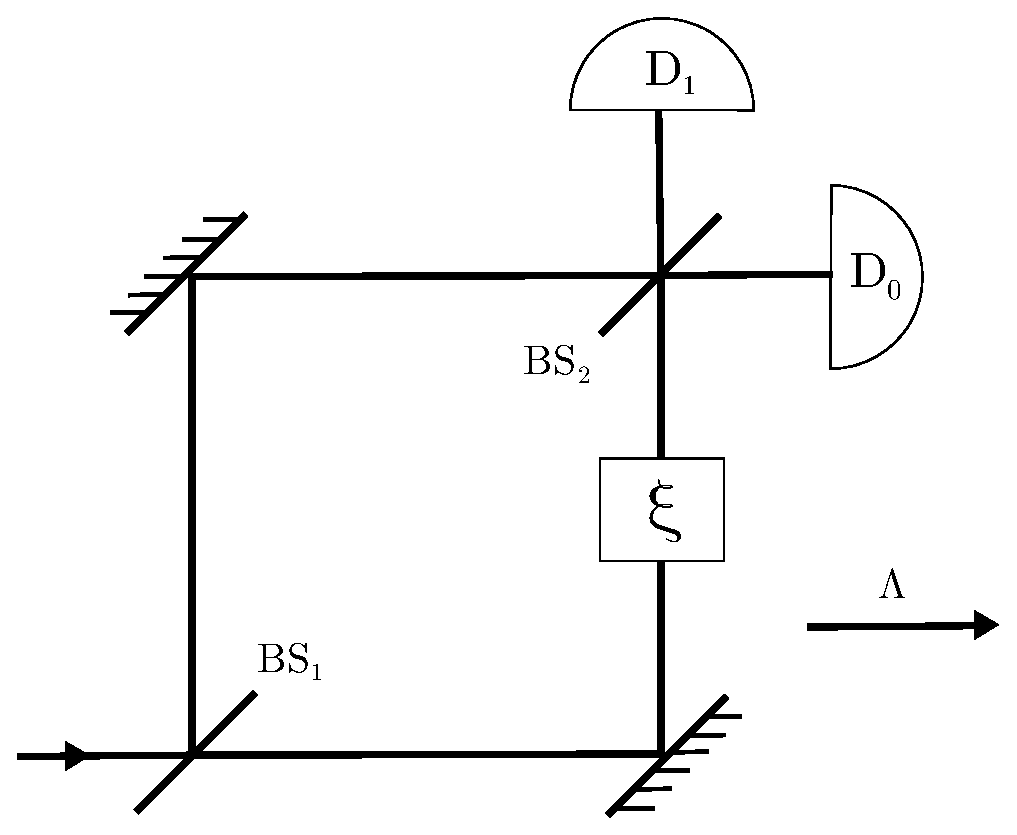
\includegraphics[scale=.45]{../Figuras/mach-zehnder-xi.eps}
  \captionsetup{font=footnotesize, margin=8pt}
  \caption{Depiction of a Mach-Zehnder interferometer and its main components: the two beam-splitters $BS_1$ and $BS_2$ and the two detectors $D_0$ and $D_1$. The mirrors add the same relative phase to both paths, so they don't contribute with any physically significant effect.}
  \label{mzi}
\end{figure}

Given the binary nature of the measurement, a qubit description is the simplest alternative to use for this system. State $\ket{0}$ is made to signify a particle in a horizontal path, and $\ket{1}$ signifies the vertical path. The action of the beam-splitters is formally described by the maps $\ket{0} \xrightarrow{BS} \frac{1}{\sqrt{2}}(\ket{0}+i\ket{1})$ and $\ket{1} \xrightarrow{BS} \frac{1}{\sqrt{2}}(\ket{1}+i\ket{0})$, and the mirrors by $\ket{0}\xrightarrow{M}i\ket{1}$ and $\ket{1}\xrightarrow{M}i\ket{0}$, so that the trajectory over the MZI of an incoming horizontal beam, up until before the second beam-splitter, is

\eq{ \ket{0} \xrightarrow{\ BS_1\ } \frac{\ket{0}+i\ket{1}}{\sqrt{2}} \xrightarrow{\ \ \ M \ \ \ } \frac{\ket{0}-i\ket{1}}{\sqrt{2}} \xrightarrow{\ \ \ \xi \ \ \ } \frac{\ket{0}-ie^{i\xi}\ket{1}}{\sqrt{2}} .
\label{mzi-states}
}
%
The action of the second beam-splitter results in

\eq{ \frac{\ket{0}-ie^{i\xi}\ket{1}}{\sqrt{2}} \xrightarrow{\ BS_2\ } &\frac{\frac{1}{\sqrt{2}}(\ket{0}+i\ket{1}) - ie^{i\xi}\frac{1}{\sqrt{2}}(\ket{1}+i\ket{0} ) }{\sqrt{2}} \nonumber \\
&= \left(\frac{1+e^{i\xi}}{2}\right)\ket{0} + i\left(\frac{1-e^{i\xi}}{2} \right)\ket{1} \nonumber \\
&= e^{i\xi/2} \left[ \cos\frac{\xi}{2}\ket{0} + \sin\frac{\xi}{2}\ket{1} \right] ,
\label{final-state}
}
%
where the global phase $e^{i\xi/2}$ can be ignored, resulting in a final state for which the probability of detection at $D_0$ is $\mathfrak{p}_0 = \cos^2(\frac{\xi}{2})$ and the complementary probability of detection at $D_1$ is $\mathfrak{p}_1 = \sin^2(\frac{\xi}{2})$. By simply adjusting the relative phase $\xi$, we can make either of the detectors completely ``dark": $\xi = 0$ results in $\mathfrak{p}_0 = 1$ and $\mathfrak{p}_1 = 0$, while $\xi = \pi$ results in $\mathfrak{p}_0 = 0$ and $\mathfrak{p}_1 = 1$.

\subsection{Quantum resource relativity in the MZI}

The above treatment of the MZI obscures the ubiquitous role of the particle's momentum in any such experiment. Since we aim to study the effects of boost-induced entanglement, we shall recast the description in terms of the (four-)momentum eigenstates defined in section \ref{four-momentum-eigenstates}. We assume that the MZI is set in the x-y plane, so that while propagating in the horizontal arms the particle's four-momentum is $p_H = (\frac{E_p}{c}, p, 0, 0)$, while in the vertical arms it is $p_V = (\frac{E_p}{c}, 0, p, 0)$. The correspondence between this and the qubit treatment is then given by the mapping $\ket{0}\rightarrow\ket{p_H}$ and $\ket{1}\rightarrow\ket{p_V}$. In particular, the state that reaches the detectors is

\eq{\label{after-bs2} \ket{\psi_f} = \cos\frac{\xi}{2}\ket{p_H} + \sin\frac{\xi}{2}\ket{p_V} .
}
%
The MZI is seen to be completely insensitive to the particle's spin state.

We now move on to consider the same experiment viewed from a reference frame $\mathcal{S}'$ moving with velocity $\vb{v} = \beta c \vu{x}$ relative to $\mathcal{S}$. The horizontal and vertical momenta seen from this frame are $\pi_H \equiv \Lambda p_H$ and $\pi_V \equiv \Lambda p_V$, which, according to \eqref{x-boost-matrix}, are given by

\eq{ \begin{split}
\label{piHpiV} \pi_H &= \left(\gamma\left(\frac{E_p}{c} - \beta p\right), \gamma\left(p - \beta \frac{E_p}{c}\right), 0, 0 \right) , \\
\pi_V &= \left(\gamma\frac{E_p}{c}, -\gamma \beta \frac{E_p}{c}, p, 0 \right) .
\end{split}
}
%
The correspondence between the quantum states on each frame is then simply obtained through equation \eqref{basis-transformation}:

\eq{\begin{split}\label{mz-transform} \ket{p_H}\ket{\Phi} &\xrightarrow{\Lambda} \ket{\pi_H}\ket{\Phi} , \\
\ket{p_V}\ket{\Phi} &\xrightarrow{\Lambda} \ket{\pi_V}\ket{\Phi_R} ,
\end{split}}
%
where $\ket{\Phi_R} \equiv R_{\vu{z}}(\Omega) \ket{\Phi}$ is the Wigner-rotated spin state, around the axis of rotation $\vu{v}\times\vu{p} = \vu{z}$. No Wigner rotation occurs in the horizontal arms of the MZI since the boost is parallel to the momentum in that case, so the spin state remains unaltered. We take the spin state in the lab frame to be $\ket{\Phi} = \cos\frac{\theta}{2}\ket{0} + e^{i\phi}\sin\frac{\theta}{2}\ket{1}$, which is an eigenstate of the spin component in the $\vu{n} = (\sin\theta\cos\phi,\sin\theta\sin\phi,\cos\theta)$ direction. The rotation around the z axis adds a relative phase $\Omega$ (the Wigner rotation angle) to the spin state, which becomes $\ket{\Phi_R} = \cos\frac{\theta}{2}\ket{0} + e^{i(\phi+\Omega)}\sin\frac{\theta}{2}\ket{1}$.

Applying transformations \eqref{mz-transform} to the state in \eqref{after-bs2}, we obtain the transformed output state $\ket*{\psi'_f}= U(\Lambda)\ket{\psi_f}$:

\eq{\label{after-bs2-l} \ket{\psi'_f} = \cos\frac{\xi}{2}\ket{\pi_H}\ket{\Phi} + \sin\frac{\xi}{2}\ket{\pi_V}\ket{\Phi_R} .
}
%
The immediate consequence of the transformation law \eqref{mz-transform}, which can be promptly noticed in the state above, is that whenever there is superposition of different momenta, there will be entanglement between spin and momentum. Tracing out the momentum, we get the spin reduced density matrix

\eq{ \rho'_S = \cos^2\frac{\xi}{2} \dyad{\Phi} + \sin^2\frac{\xi}{2} \dyad{\Phi_R},
}
whose von Neumann entropy gives the entanglement between spin and momentum:

\eq{ S(\rho'_S) = h\Bigg(\frac{1}{2} + \frac{1}{8}\sqrt{2\bigg(7 + \cos\Omega + 2(\cos(2\xi) + 2\cos(2\theta)\sin^2\xi)\sin^2\frac{\Omega}{2}\bigg)} \Bigg) ,
}
%
where $h(x)$ is the binary entropy. Figure \ref{3d-plots} shows $S(\rho'_S)$ as a function of the boost velocity $\beta$ (which controls the angle $\Omega$), the spin polar angle $\theta$ and the MZI phase $\xi$. After interference on the second beam-splitter, the superposition of momentum is dictated by the phase $\xi$, with the values $\xi = 0$ and $\xi = \pi$ resulting in $100\%$ detection rate on detectors $D_0$ and $D_1$, respectively. As there is no superposition of momentum, these cases do not generate entanglement. Another less obvious case in which there is no entanglement is when $\theta \in \{0, \pi \}$ (i.e., when the spin state is either $\ket{0}$ or $\ket{1}$). That is because the Wigner rotation is around the z-axis, so it leaves $\sigma_z$ eigenstates invariant. The values $\xi = \frac{\pi}{2}$ and $\theta = \frac{\pi}{2}$ maximize the entanglement effect. For these values, the entropy of entanglement gives

\eq{ S(\rho'_S) &= h\left(\cos^2\frac{\Omega}{4}\right) \nonumber \\
&= -\cos^2\frac{\Omega}{4} \log_2\left(\cos^2\frac{\Omega}{4}\right) -  \sin^2\frac{\Omega}{4}\log_2 \left(\sin^2\frac{\Omega}{4}\right).
}
%
%
\begin{figure}[t]
  \centering
  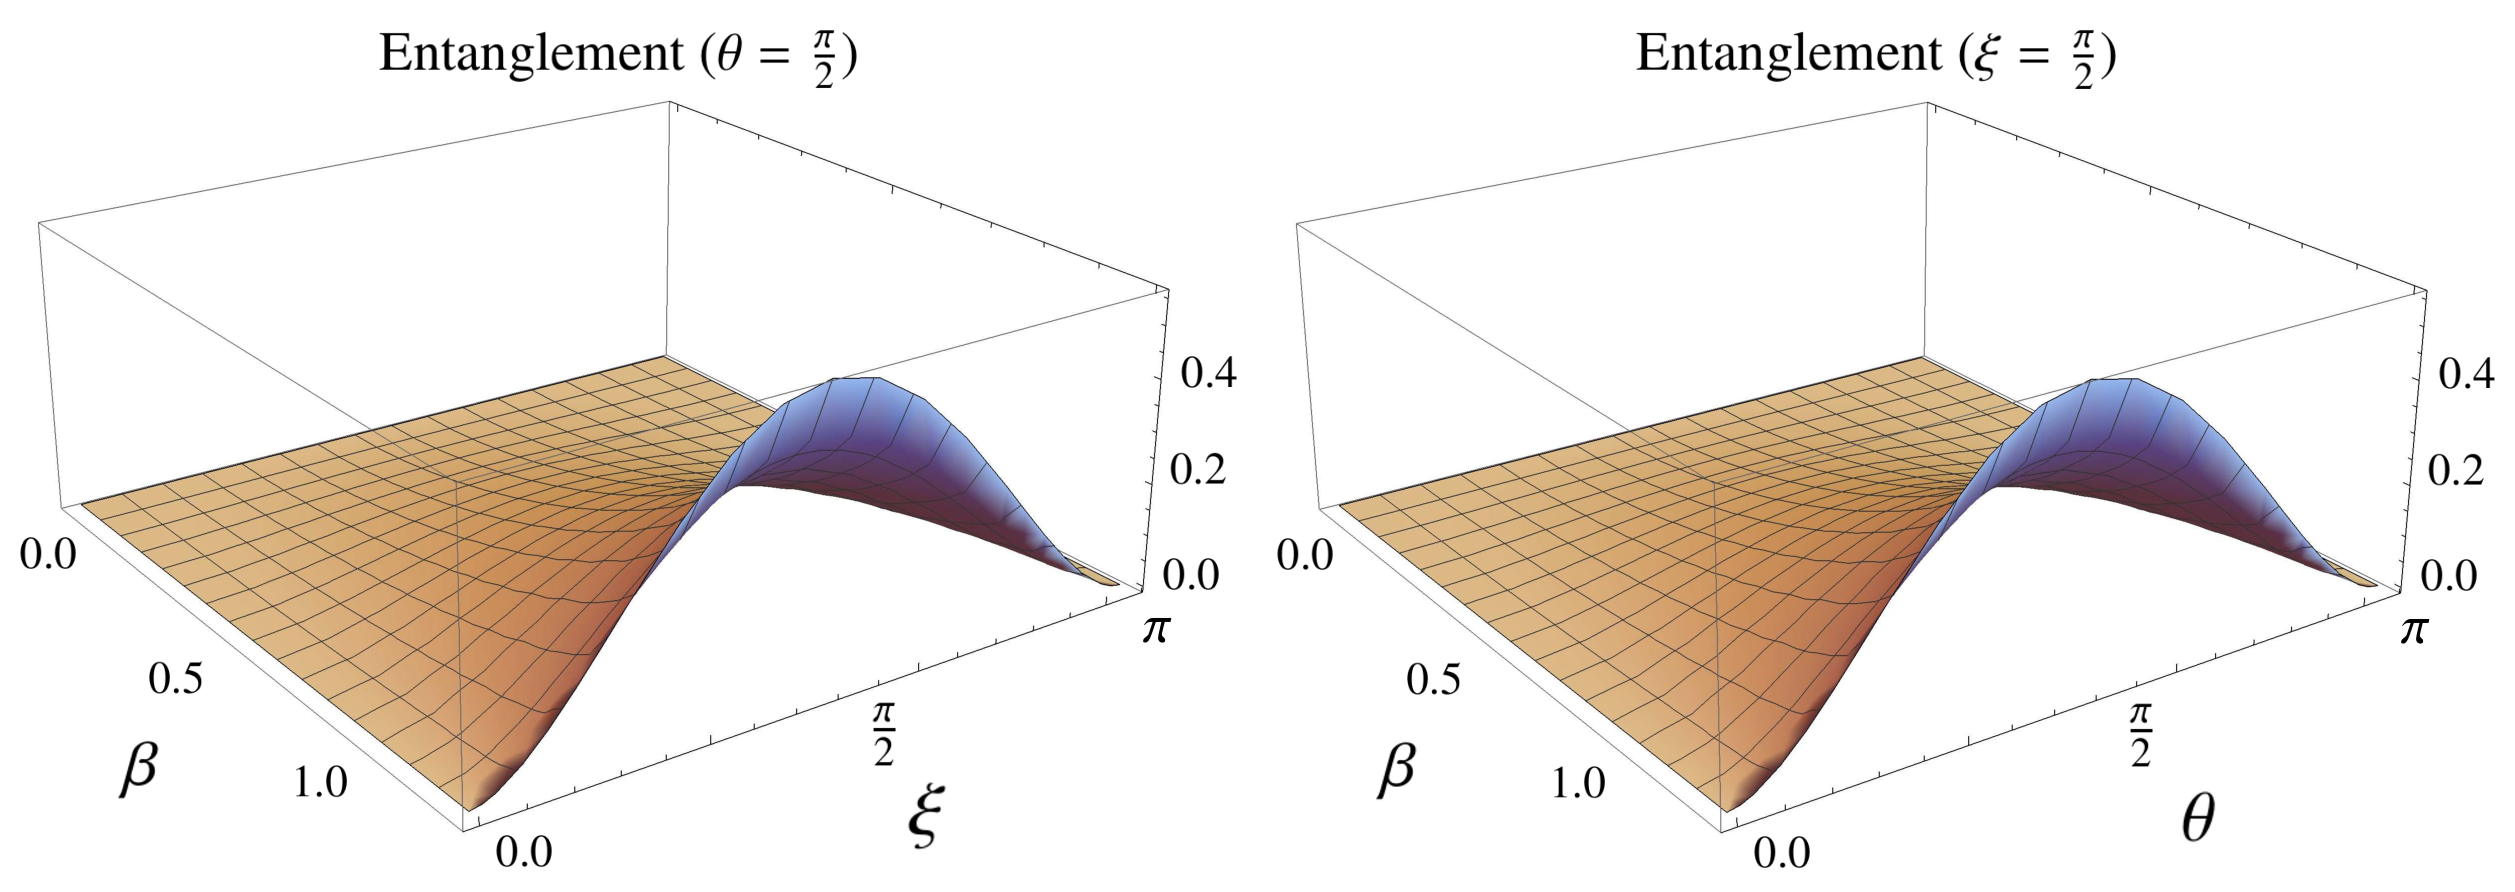
\includegraphics[scale=.37]{../Figuras/improved/3d-plots-IMPROVED.eps}
  \captionsetup{font=footnotesize, margin=8pt}
  \caption{Entropy of entanglement between spin and momentum for the output state of the MZI in the boosted reference frame $\mathcal{S}'$. On the left, the initial spin state is in the equator of the Bloch sphere ($\theta=\frac{\pi}{2}$) and $S(\rho_S)$ is plotted as function of the phase $\xi$ and boost velocity $\beta$. On the right, the phase $\xi$ is held constant ($\xi = \frac{\pi}{2}$) and $S(\rho_S)$ is plotted as function of $\theta$ and $\beta$. Entanglement is shown to increase with the boost velocity in general, except for very specific geometric  configurations.}
  \label{3d-plots}
\end{figure}
%

\subsection{Relativity of reality in the MZI}

Just like was done for the last example, we will now investigate the ontological status of spin and momentum, as per BA's criterion of realism and irreality quantifier, equations \eqref{real} and \eqref{irreality}, respectively.
The spin component $\sigma_{\vu{n}} = \vu{n}\cdot\vb*{\sigma}$ is always an element of reality in the lab frame; that is, when $\beta = 0$, we have

\eq{ \Phi_{\sigma_{\vu{n}}}(\rho) = \rho,
}
%
for $\rho = \dyad{\psi_f}$. For the output state in the moving frame, $\rho' = \dyad*{\psi'_f}$, the irreality of $\sigma_{\vu{n}}$ increases with the Wigner rotation angle:

\eq{\label{sigma-irr}  \mathfrak{I}_{\sigma_{\vu{n}}}(\rho')  = h\left(\sin^2\theta\ \sin^2\frac{\xi}{2} \ \sin^2\frac{\Omega}{2}\right) .
}
%
The dependence on $\theta$ is due to the same reason explained before: $\sigma_z$ eigenstates are unaffected by the Wigner rotation due to the specific geometric configuration considered here. The dependence on $\xi$ is more interesting: while entanglement is maximized for $\xi=\frac{\pi}{2}$ and is zero for $\xi=\pi$, the irreality of $\sigma_{\vu{n}}$ is maximal for $\xi=\pi$, when only the vertical detector $D_1$ is reached with probability 1. Since no correlations are present, all of the irreality in this case is due to $\sigma_{\vu{n}}$-coherence being generated by the rotation. In fact, for the relative entropy of coherence $\mathbb{C}_{\sigma_{\vu{n}}}(\rho'_S) = S(\Phi_{\vu{n}}(\rho'_S)) - S(\rho'_S)$, the term $S(\Phi_{\vu{n}}(\rho'_S))$ evaluates to the same expression as \eqref{sigma-irr}, such that when there is no entanglement ($S(\rho'_S) = 0$) the spin irreality is fully attributed to coherence.

We may also ask about the reality status of the momentum, by treating each momentum component by its own Hilbert space, similarly to what has recently been done in \cite{petreca_2021}. Rewritting the state in \eqref{after-bs2} in a more complete notation, which makes explicit each component of the four-momentum, we have

\eq{\nonumber \ket{\psi_f} &= \cos\frac{\xi}{2}\ket{p_H} + \sin\frac{\xi}{2}\ket{p_V} \\
&= \cos\frac{\xi}{2}\ket{\tfrac{E_p}{c}, p, 0, 0} + \sin\frac{\xi}{2}\ket{\tfrac{E_p}{c}, 0, p, 0},
\label{rest-components}
}
%
from which we see that the energy and the z component are the same in both branches of the superposition, meaning they can be factorized and essentially ignored. The x and y component, on the other hand, are entangled with each other. Within the discretized framework we have been using, the only accesible states for the $x$ and $y$ components are $\ket{0}_{x(y)}$ and $\ket{p}_{x(y)}$, meaning that each component behaves as a qubit. The entropy of entanglement between these parts gives $S(\rho_{P_x}) = S(\rho_{P_y}) = h(\cos^2\frac{\xi}{2})$, which is zero when $\xi \in \{ 0,\pi \}$ and maximal ($S(\rho_{P_x}) = 1$) when $\xi = \frac{\pi}{2}$. The same expression gives the total irreality of each momentum component: $\mathfrak{I}_{P_x}(\rho) = \mathfrak{I}_{P_y}(\rho) = h(\cos^2\frac{\xi}{2})$, with both being elements of reality when $\xi \in \{0, \pi \}$. As for the moving frame $\mathcal{S}'$, the transformed state in \eqref{after-bs2} can also be rewritten in terms of the momentum components with the aid of \eqref{piHpiV}:

\eq{\nonumber \ket{\psi'_f} &= \cos\frac{\xi}{2}\ket{\gamma\left(\tfrac{E_p}{c} - \beta p\right), \gamma\left(p - \beta \tfrac{E_p}{c}\right), 0, 0}\ket{\Phi} + \sin\frac{\xi}{2}\ket{\gamma\tfrac{E_p}{c}, -\gamma \beta \tfrac{E_p}{c}, p, 0 }\ket{\Phi_R} \\
&\equiv \cos\frac{\xi}{2}\ket{\pi_H^0, \pi_H^x, 0, 0}\ket{\Phi} + \sin\frac{\xi}{2}\ket{\pi_V^0, \pi_V^x, \pi_V^y, 0 }\ket{\Phi_R} .
}
%
Here we notice something unexpected: while the z component remains unaffected by the boost, the zero-component (energy) is not the same for $\pi_H$ and $\pi_V$, showing that a Lorentz boost may also create entanglement between energy and momentum. Notice that this doesn't happen in the example studied in the last section. There, the boost was perpendicular to both superposed momentum states, such that after the boost, the energy of both branches was changed by the same factor, remaining separable from the other components.

The irreality of $P_x$ and $P_y$ are both independent of the boost, and equal to the same value as in the lab frame: $\mathfrak{I}_{P_x}(\rho') = \mathfrak{I}_{P_y}(\rho') = h(\cos^2\frac{\xi}{2})$. Likewise, the entanglement between one of these momentum components and the rest of the degrees of freedom is also boost-independent and equal to the same expression $S(\rho'_{P_x}) = S(\rho'_{P_y}) = h(\cos^2\frac{\xi}{2})$. The energy, which is an element of reality in the lab frame, presents entanglement and irreality in the moving frame, with an equal dependence on $\xi$ as the components $P_x$ and $P_y$: $S(\rho'_{P_0}) = \mathfrak{I}_{P_0}(\rho') = h(\cos^2\frac{\xi}{2})$. We can conclude that, for the momentum degree of freedom, entanglement and irreality in the output state of the MZI is entirely dictaded by the phase $\xi$. In other words, both reference frames agree that the momentum ontology is determined solely by the characteristics installed in the MZI.


\subsection{Paradox concerning spin measurements in the MZI}

As discussed in the first section of this chapter, the type of entanglement induced by Lorentz boosts cannot be detected through an observable difference in the momentum probability density in an interference experiment. In fact, it was verified that the probabilities for each MZI detector clicking were the same in both frames, dependent only on the phase $\xi$. One might ask, then, if there is any way to experimentally verify the strange effects of the Wigner rotation in the MZI, perhaps using spin-sensitive detectors. To this end, consider a slightly modified MZI setup in which the detectors $D_0$ and $D_1$ now measure the $\vu{n}$ component of spin (i.e. they are $\vu{n}$-directed spin detectors). In the lab frame, since the spin state $\ket{\Phi}$ is an eigenstate of $\sigma_{\vu{n}}$, the detectors will always record a ``spin up" result, regardless of the output port of the interferometer. In accordance with the state in \eqref{after-bs2}, the probability of detection at $D_0$ is $\mathfrak{p}_0 = \cos^2\frac{\xi}{2}$ and at $D_1$, $\mathfrak{p}_1 = \sin^2\frac{\xi}{2}$.

In the moving frame $\mathcal{S}'$, the state that reaches the detectors is given by \eqref{after-bs2-l}:

\eq{\tag{\ref{after-bs2-l}} \ket{\psi'_f} = \cos\frac{\xi}{2}\ket{\pi_H}\ket{\Phi} + \sin\frac{\xi}{2}\ket{\pi_V}\ket{\Phi_R} .
}
%
Just like in the lab frame $\mathcal{S}$, there is a probability of $\cos^2\frac{\xi}{2}$ that the particle will be detected at $D_0$, in which case its spin state is $\ket{\Phi}$, resulting in a definite ``spin up" detection. If the particle is to be found in the vertical detector $D_1$, however, its spin state will be $\ket{\Phi_R}$. There will then be a probability $\Tr[(1-\dyad{\Phi})\dyad{\Phi_R}] = 1-\left|\bra{\Phi}\ket{\Phi_R}\right|^2 = \sin^2\theta\sin^2\frac{\Omega}{2}$ that the spin detector will record a ``spin down" result. This shows a disagreement between the observations made in the two reference frames, implying a paradoxical disagreement in the events counting.

To solve this paradox, we first need to address the question of what it means to measure a spin component. The simplest physical setup that implements a spin measurement as idealized above is the Stern-Gerlach (SG) experiment. As discussed in section \ref{stern-gerlach}, the mechanism by which the SG enables spin to be measured is through entanglement with momentum, which acts as an informer degree of freedom. By taking into account the momentum imparted onto the particle by the SG we will verify that the two reference frames indeed agree on the result of the measurements at the end of the MZI.

The spin measurement of the SG amounts to the discrimination between two different momenta that can leave the SG apparatus. For a measurement of the $\vu{n}$-component of spin, the non-homogeneous magnetic field is aligned in the $\vu{n}$ direction, which applies an impulse $\vb{q}_{\pm} = \pm q \vu{n}$ on the particle, depending on the orientation of its spin. If a particle enters with momentum $\vb{p}$, the value of spin is inferred from the output momentum, which is either $\vb{p}_+ = \vb{p} + \vb{q}_+$ or $\vb{p}_- = \vb{p} + \vb{q}_-$ (see figure \ref{sg-fig}). Defining $U_{SG}$ to be the unitary operator that effects the dynamics of the SG, its action on the $\sigma_{\vu{n}}$ eigenstates, $\ket{\Phi}$ and $\ket{\Phi_{\bot}}$, is

\eq{\begin{split} &U_{SG}\ket{p, \Phi} = \ket{p_+, \Phi}, \\
&U_{SG}\ket{p, \Phi_\bot} = \ket{p_-, \Phi_\bot},
\end{split}
}
%
where $p_{+(-)}$ is simply the four-vector associated with the imparted three-momentum $\vb{p}_{+(-)}$.
So in frame $S$, the state that arrives at the detectors is transformed by $U_{SG}$ in the following way:

\eq{\label{sg-state-s} U_{SG}\left( \cos\frac{\xi}{2} \ket{p_H, \Phi} + \sin\frac{\xi}{2} \ket{p_V, \Phi} \right) =  \cos\frac{\xi}{2}\ket{p^+_H, \Phi} + \sin\frac{\xi}{2}\ket{p^+_V, \Phi} ,
}
%
so that the resulting momenta indicate a spin up result ($p^+_{H(V)}$, as opposed to $p^-_{H(V)}$). Meanwhile, the measurement result in frame $\mathcal{S}'$ is found by transforming the state \eqref{sg-state-s}:

\eq{\label{sg-state-sl} U(\Lambda) \left( \cos\frac{\xi}{2}\ket{p^+_H, \Phi} + \sin\frac{\xi}{2}\ket{p^+_V, \Phi} \right) = \cos\frac{\xi}{2}\ket{\pi^+_H, \Phi_{R1}} + \sin\frac{\xi}{2}\ket{\pi^+_V, \Phi_{R2}} .
}
%
Here, $\ket{\Phi_{R1}}$ and $\ket{\Phi_{R2}}$ denote different theoretically predicted, Wigner-rotated spin states. However, as we already established, at this point of the experiment the only thing that is directly accessed is the particle's momentum, from which the value of $\sigma_{\vu{n}}$ is inferred.
Just like in frame $\mathcal{S}$, where the measurement is dependent on the discrimination between different momenta $p_+$ and $p_-$, in frame $\mathcal{S}'$, the same measurement depends on the discrimination between $\pi_+$ and $\pi_-$. As such, state \eqref{sg-state-sl} tells us that the moving frame agrees about the spin up result, thereby resolving the paradox.

\begin{figure}[t]
  \centering
  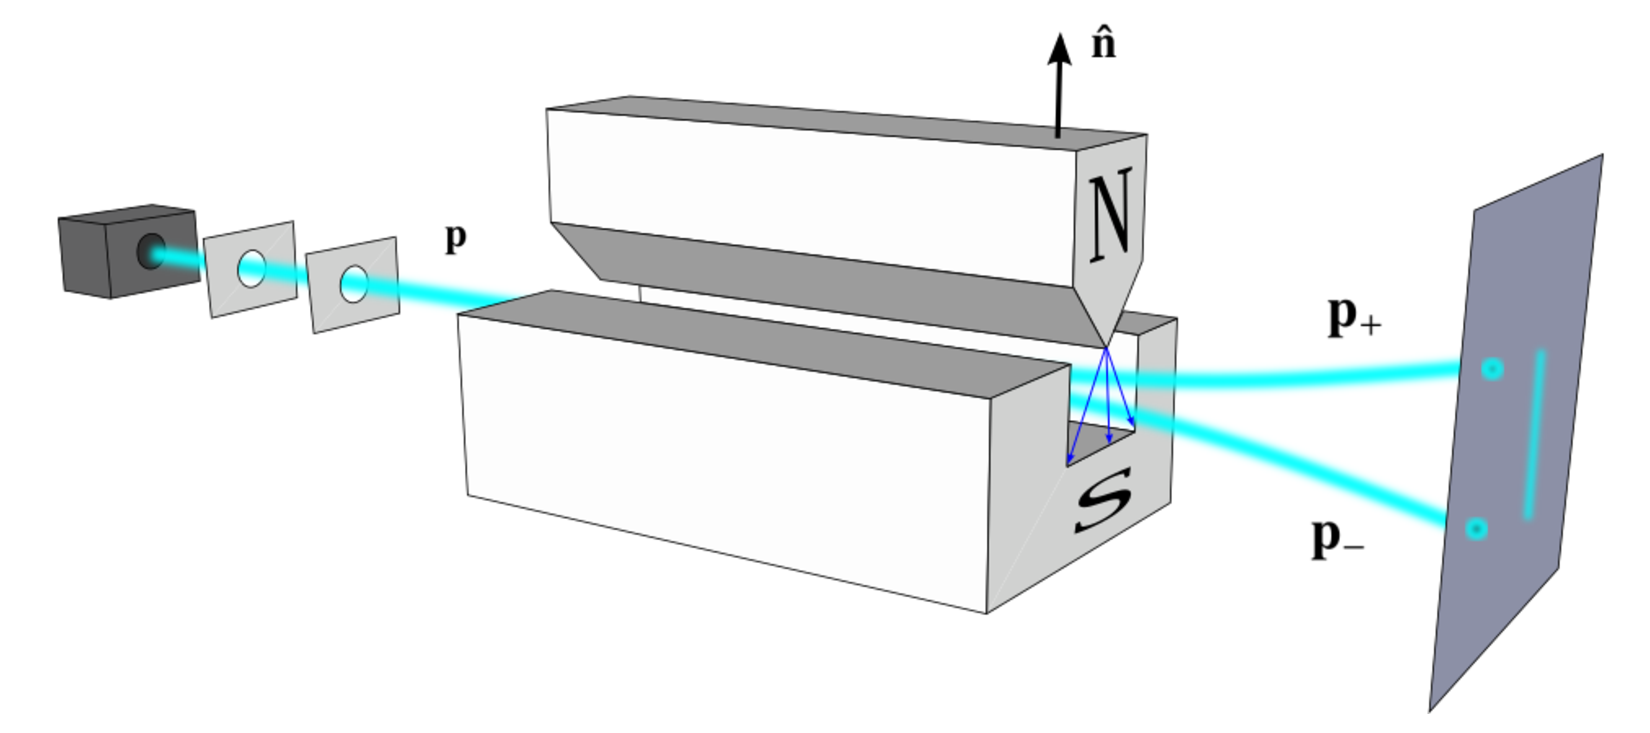
\includegraphics[width=.8\textwidth]{../Figuras/SG_f.eps}
  \captionsetup{font=footnotesize, margin=8pt}
  \caption{Visual depiction of the Stern-Gerlach experiment, used to measure spin along the $\vu{n}$ direction. The incoming beam and the two output beams are defined by their momenta, and the value of $\sigma_{\vu{n}}$ (either +1 or -1) is inferred from the arrival position at the detection plate (equivalently, from the momentum of the output beam).}
  \label{sg-fig}
\end{figure}

\subsection{General boost scenarios}

One special feature, particular to this case study, is that the momenta in superposition are perpendicular to each other. This has the implication that, for any boost direction, there will always be a Wigner rotation taking place. This is in contrast to most usual systems investigated in relativistic quantum information. On the previous case study, for example, a boost along the z axis would provide no interesting results, since it would be parallel to the particle's momentum (for all branches of the momentum superposition) and thus no Wigner rotation would affect the spin state. For the MZI, whatever direction the boost is in, there will always be a non-parallel momentum component for which the spin will undergo a rotation. Considering a boost in a general direction $\vu*{\beta}$, the state at the output of the MZI reads

\eq{ \ket{\psi'_f} = \cos\frac{\xi}{2} \ket{\Lambda p_H} \ket{\Phi_H} + \sin\frac{\xi}{2}\ket{\Lambda p_V} \ket{\Phi_V} ,
}
%
with $\ket{\Phi_H} \equiv R_{\vu{n}_x}(\Omega_x) \ket{\Phi}$ being the spin state in the horizontal output, rotated around the axis $\vu{n}_x = \vu{x}\times\vu*{\beta}$, and $\ket{\Phi_V} \equiv R_{\vu{n}_y}(\Omega_y) \ket{\Phi}$ being the spin state in the vertical output, rotated around $\vu{n}_y = \vu{y}\times\vu*{\beta}$. Recalling the orthonormality of the momentum states, the reduced density matrix for spin can be easily obtained:

\eq{ \rho'_S = \cos^2\frac{\xi}{2} \dyad{\Phi_H} + \sin^2\frac{\xi}{2} \dyad{\Phi_V} .
}

Simple as it may look, the state above presents significant challenges when it comes to calculating its von Neumann entropy. This is due to difficulties in obtaining the states $\ket{\Phi_H}$ and $\ket{\Phi_V}$ in the $\sigma_{\vu{n}}$ basis, the main issues being:

\begin{enumerate}

\item We now have two Wigner rotations, with different angles $\Omega_x$ and $\Omega_y$;

\item Each rotation depends on two new parameters (two angles specifying the direction $\vu*{\beta}$ of the boost), in addition to the three usual parameters $\theta$, $\phi$ and $\xi$, plus the two angles;

\item In general, the boost is not perpendicular to either momenta $p_H$ and $p_V$, which means that neither of the angles $\Omega_x$ and $\Omega_y$ can be obtained by the simplified formula \eqref{omega-neat}. Instead, we must rely on the much more complicated general form given in \eqref{omega}.

\end{enumerate}

Instead of letting these difficulties hinder our analysis, we can procceed without explicitly obtaining the Wigner-rotated spin states. For this, instead of using the von Neumann entropy, we quantify the mixedness of the reduced state using the linear entropy, $S_L = 1 - \Tr(\rho_S^2)$, which is far easier to compute and provides roughly the same information. From it, we obtain the following expression for the entanglement:

\eq{ E(\ket*{\psi'_f}) = \frac{1}{2}\left( 1 - \left|\bra{\Phi_H}\ket{\Phi_V}\right|^2 \right)\sin^2\xi.
}
%
As expected, the term $\sin^2\xi$ guarantees that whenever there is no superposition of momenta (only one of the detectors clicks, $\xi \in \{0 , \pi \}$), no entanglement is present. Entanglement is otherwise dictated by the term $\left|\bra{\Phi_H}\ket{\Phi_V}\right|^2$. This is equal to one (implying zero entanglement) if and only if the boost velocity is zero, in which case $\ket{\Phi_x} = \ket{\Phi_y} = \ket{\Phi}$. For any $\beta > 0$, $\ket{\Phi_H}$ and $\ket{\Phi_V}$ will be different, and $E(\ket*{\psi'_f}) > 0$. Unfortunately, quantum coherence and irreality must necessarily employ the von Neumann entropy in their quantifiers. However, by certifying that entanglement is generated for all boost directions, we can expect the same feature for coherence and irreality. Proving such results analytically, as well as determining the specific dependence on the boost direction $\vu*{\beta}$, constitues a possible direction for extending this research program.

\pagebreak


\chapter{Conclusions}


The type of phenomenon studied in this and other works of relativistic quantum information refers to systems found in an intersection of extreme limits of nature; the controlled and isolated regimes of QM, and the high energies and high velocities regimes of special relativity. While this presents a challenge when it comes to experimental verification and present-day applications, the advancements in Quantum Computation promise to drive our technologies closer and closer to these extreme limits.

When we eventually reach this technological landmark, it will be of vital importance to understand exactly how the quantum resources utilized in information processing tasks are affected by a change of reference frame. But the scope of this work goes beyond technological applications. We are instead interested in investigating fundamental questions that lie within the heart of foundational physics, while also approaching philosophical disciplines like ontology.


By directly calculating the Lorentz transformation of quantum single-particle states, we verified what has been a prominent conclusion in the literature for the past two decades, namely, that quantum resources (specifically entanglement) are not Lorentz invariant quantities. In addition to that, we verified that quantum irreality, as quantified by BA, and quantum coherence, are also not Lorentz invariant. All of these quantities have no generally accepted covariant transformation law, which means that their definitions should not be taken as statements of physical laws in the general sense. Instead, their definition is based on their utility for computational tasks, and it is from this utility that we derive the importance of understanding how these quantities are affected by a change of reference frames.

To study the irreality of the four-momentum, we treated each of the four components by its own Hilbert space. This treatment, albeit rigorous and in consonance with standard QM, is not commonly seen on other works of relativistic quantum mechanics (with the recent exception of \cite{petreca_2021}, where multipartite entanglement and coherence were studied for an electron-positron pair). Using this approach, we verified a different facet of the entangling effects of Lorentz boosts: the energy irreality increases with the boost, and energy can become entangled with the other components of the four-momentum.

In regards to experimental observability, we addressed two sensible guesses about what may be observable consequences of the boost.
Firstly, we considered the possibility that the two reference frames may observe different interference patterns (due to one of them observing momentum entanglement, while for the other one, momentum is separable). This was discarded due to the unitarity of the transformation guaranteeing the same probability density in both frames, which allowed us to conclude that boost-induced entanglement is a non-decohering type of entanglement.

Secondly, we conceived a setup involving spin measurements in a Mach-Zehnder interferometer, which seemed to utilize the difference in spin entanglement between the two frames in a way that implied different detection probabilities (i.e. a paradoxical violation of relativity). We solved this paradox by adopting a fully operational point of view, considering the physical implementation of the spin measurements (i.e. the Stern-Gerlach setup) and the role of spin-momentum entanglement in any such experiment.


The type of entanglement studied in this work, between the spin and momentum of a single particle, is not of direct applicability to quantum information and quantum computation: there, the useful forms of entanglement are between two or more qubits (i.e. entanglement between the spin of two or more particles). It has been shown, however, that this effect has non trivial consequences for multi-particle entanglement. A driving factor for those consequences is the fact that internal entanglement and external entanglement obey a monogamy relation (i.e. there is a tradeoff between the two, in which one limits the other), a relatively recent result in the literature \cite{camalet_2018, zhu_2020}. This suggests a promising direction for further developments: the study of quantum resources and quantum irreality of multi-particle systems. In addition to considering more particles, another natural extension to this research program would be to consider mixed states, since they are more representative of actual quantum systems (more general than pure states, which are an idealization), and therefore would extend the generality of the results. Additionally, the entanglement, coherence and irreality considered in this work may have a role in a possible informational invariant to be discovered. If such an invariant quantity exists (and it is expected to exist), its discovery will be contingent on a good understanding of how these resources are transmuted under a boost.


\appendix

\chapter{Momentum discretization made rigorous}
\label{app-a}

In section \ref{opposite-momenta}, the simplicity of the physical system in consideration allowed us to treat the particle's momentum as a qubit, with a two-dimensional Hilbert space spanned by orthonormal vectors $\ket{p_+}$ and $\ket{p_-}$. In this appendix we will prove the validity of this treatment, by making explicit the bridge between this and the general, continuous treatment of section \ref{gen-states}.

Consider the following ``relativistic delta function":

\eq{ \delta_R(\vb{p}_0) := 2 p_0 \delta^3(\vb{p}-\vb{p}_0).
}
It can be immediately verified that $\delta_R(\vb{p}_0)$ is normalized according to the Lorentz invariant integration measure $\dd{\mu(\vb{p})} = \dd[3]{\vb{p}}/2 p_0$:

\eq{ \int \delta_R(\vb{p}_0) \dd{\mu(\vb{p})} = \int \delta^3(\vb{p}-\vb{p}_0) \dd[3]{\vb{p}} = 1 .
}
%
This shows that $\delta_R(\vb{p}_0)$ qualifies as being a valid relativistic probability density, corresponding to the particle having a well defined momentum $\vb{p}_0$. 

Next, consider the following two-component wave function:

\eq{\begin{split}
\label{qubit-wavefunction} \psi_0(\vb{p}) &= \frac{\sqrt{\delta_R(\vb{p}_+)} + \sqrt{\delta_R(\vb{p}_-)}}{\sqrt{2}}, \\
\psi_1(\vb{p}) &= 0 .
\end{split}
}
%
The corresponding probability density is

\eq{ |\psi_0(\vb{p})|^2 + |\psi_1(\vb{p})|^2 = \frac{\delta_R(\vb{p}_+) + \delta_R(\vb{p}_-) + 2\sqrt{\delta_R(\vb{p}_+)\delta_R(\vb{p}_-)}}{2},
}
%
which is correctly normalized according to the Lorentz invariant integration measure, and represents a probability $\frac{1}{2}$ of finding the particle with momentum $\vb{p}_+$ and an equal probability $\frac{1}{2}$ to find it with momentum $\vb{p}_-$. As for the spin, the probability of finding spin up is $\int|\psi_0(\vb{p})|^2\dd{\mu(\vb{p})} = 1$. If we assume that the spin basis used for the representation of the state in \eqref{qubit-wavefunction} is the $\sigma_{\vu{n}}$ basis, for which $\ket{\Phi}$ is the spin up state, then \eqref{qubit-wavefunction} provides the complete, rigorous version of the state in \eqref{opposite-momenta-state}.

To convince ourselves of the equivalence between \eqref{qubit-wavefunction} and \eqref{opposite-momenta-state}, we will proceed with the calculation of the spin reduced density matrix in this rigorous approach. Firstly, the boost transformed wave function is given by \eqref{gen-transf-wf}:

\eq{ \phi_{\sigma'}(\vb*{\Lambda}\vb{p}) \equiv \sum_\sigma D_{\sigma' \sigma}(\Lambda, \vb{p}) \psi_\sigma (\vb{p}),
}
where $D(\Lambda, \vb{p})$ is the Wigner rotation matrix. With $\psi_1(\vb{p}) = 0$, the transformed wave function is simply

\eq{\label{transf-a} \phi_0(\vb*{\Lambda}\vb{p}) &= D_{00}(\Lambda, \vb{p}) \psi_0(\vb{p}) = \frac{D_{00}(\Lambda, \vb{p}_+)\sqrt{\delta_R(\vb{p}_+)} + D_{00}(\Lambda, \vb{p}_-)\sqrt{\delta_R(\vb{p}_-)}}{\sqrt{2}}, \\
\phi_1(\vb*{\Lambda}\vb{p}) &= D_{10}(\Lambda, \vb{p}) \psi_0(\vb{p}) = \frac{D_{10}(\Lambda, \vb{p}_+)\sqrt{\delta_R(\vb{p}_+)} + D_{10}(\Lambda, \vb{p}_-)\sqrt{\delta_R(\vb{p}_-)}}{\sqrt{2}}.
\label{transf-b}}
%
Recalling that the momenta $\vb{p}_{\pm}$ are in the z direction and the boost is in the x direction, the rotations $D(\Lambda, \vb{p}_+)$ and $D(\Lambda, \vb{p}_-)$ will be both around the y axis, but in opposite directions; that is

\eq{\begin{split} D(\Lambda, \vb{p}_{\pm}) &= \cos\frac{\Omega}{2} \pm i \sin\frac{\Omega}{2} \sigma_y  \\
&= \begin{bmatrix}[1.7] \cos\frac{\Omega}{2} & \pm  \sin\frac{\Omega}{2} \\ 
\mp \sin\frac{\Omega}{2} & \cos\frac{\Omega}{2} \end{bmatrix}.
\label{dz}
\end{split}
}
%
However, we already established that the spin basis we are using for the state \eqref{qubit-wavefunction} is the $\sigma_{\vu{n}}$ eigenbasis, so we need to express $D(\Lambda, \vb{p}_{\pm})$ in this same basis. The matrix that changes from the $\sigma_z$ to the $\sigma_{\vu{n}}$ basis is

\eq{ T = \begin{bmatrix}[1.7]  \bra{0}\ket{\Phi} & \bra{0}\ket{\Phi_{\bot}} \\
\bra{1}\ket{\Phi} & \bra{1}\ket{\Phi_{\bot}} \end{bmatrix} = \begin{bmatrix}[1.7]  \cos\frac{\theta}{2} & \sin\frac{\theta}{2} \\
e^{i\phi}\sin\frac{\theta}{2} & -e^{i\phi}\cos\frac{\theta}{2} \end{bmatrix}.
}
%
The Wigner rotation matrix in the $\sigma_{\vu{n}}$ basis, $D_{\vu{n}}$, is related to the same matrix in the $\sigma_z$ basis, $D_z$ (equation \eqref{dz}), through $D_{\vu{n}} = T^{-1}D_zT$. Explicitly:

\eq{ D_{\vu{n}} = \begin{bmatrix}[1.7]   \cos\frac{\theta}{2} & e^{-i\phi}\sin\frac{\theta}{2} \\
\sin\frac{\theta}{2} & -e^{i\phi}\cos\frac{\theta}{2} \end{bmatrix} \begin{bmatrix}[1.7] \cos\frac{\Omega}{2} & \pm \sin\frac{\Omega}{2} \\ 
\mp \sin\frac{\Omega}{2} & \cos\frac{\Omega}{2} \end{bmatrix} \begin{bmatrix}[1.7]   \cos\frac{\theta}{2} & \sin\frac{\theta}{2} \\
e^{i\phi}\sin\frac{\theta}{2} & -e^{i\phi}\cos\frac{\theta}{2} \end{bmatrix} \nonumber \\
= \begin{bmatrix}[1.7] \cos\frac{\Omega}{2} \pm i \sin\theta\sin\phi\sin\frac{\Omega}{2} & \mp(\cos\phi+i\cos\theta\sin\phi)\sin\frac{\Omega}{2} \\
\pm(\cos\phi-i\cos\theta\sin\phi)\sin\frac{\Omega}{2} & \cos\frac{\Omega}{2} \mp i \sin\theta\sin\phi\sin\frac{\Omega}{2} \end{bmatrix},
}
%
from which we finally obtain the matrix elements that appear in \eqref{transf-a} and \eqref{transf-b}:

\eq{\label{d00} D_{00}(\Lambda, \vb{p}_{\pm}) &= \cos\frac{\Omega}{2} \pm i\sin\theta\sin\phi\sin\frac{\Omega}{2}, \\ 
D_{10}(\Lambda, \vb{p}_{\pm}) &= \pm(\cos\phi -i\cos\theta\sin\phi)\sin\frac{\Omega}{2}.
\label{d10}
}
%
Instead of substituting these into \eqref{transf-a} and \eqref{transf-b} right away, let us step back and refocus on our main calculational goal, which is to obtain the spin reduced density matrix of equation \eqref{sdm-example2}.

The complete (spin and momentum) density matrix associated with the wave function $\phi_{\sigma}(\vb{p})$ is

\eq{ \rho(\vb{p},\vb{q}) \stackrel{\cdot}{=} \begin{bmatrix}[1.7] \phi_0(\vb{p})\phi_0^*(\vb{q}) & \phi_0(\vb{p})\phi_1^*(\vb{q}) \\
\phi_1(\vb{p})\phi_0^*(\vb{q}) & \phi_1(\vb{p})\phi_1^*(\vb{q})
\end{bmatrix}.
}
%
Tracing out the momentum amounts to setting $\vb{p} = \vb{q}$ and integrating; that is, the spin reduced density matrix is

\eq{ \rho_S \stackrel{\cdot}{=} \begin{bmatrix}[1.7] \int|\phi_0(\vb{p})|^2\dd{\mu(\vb{p})} & \int\phi_0(\vb{p})\phi^*_1(\vb{p})\dd{\mu(\vb{p})} \\
\int\phi_1(\vb{p})\phi^*_0(\vb{p})\dd{\mu(\vb{p})} & \int|\phi_1(\vb{p})|^2\dd{\mu(\vb{p})}
\end{bmatrix}.
}
%
We need only calculate two of these matrix elements; one in the diagonal, from which the other one is fixed by the normalization requirement $\Tr(\rho_S) = 1$, and one off diagonal, from which the other is fixed by the hermiticity requirement $\rho_S^\dagger = \rho_S$. First we evaluate $|\phi_0(\vb{p})|^2$ by taking \eqref{transf-a} and multiplying by its complex conjugate. The result is

\eq{ |\phi_0(\vb{p})|^2 =  \frac{1}{2} \Big\{ |D_{00}(\Lambda, \vb{p}_+)|^2\delta_R(\vb{p}_+) + |D_{00}(\Lambda, \vb{p}_-)|^2\delta_R(\vb{p}_-) + ... \Big\} ,
}
%
where the ommited terms involve products $\sqrt{\delta_R(\vb{p}_+)\delta_R(\vb{p}_-)}$ that won't contribute to the integration. After integration, this becomes the first element of the reduced density matrix:

\eq{ \rho_{S00} &= \frac{|D_{00}(\Lambda, \vb{p}_+)|^2 + |D_{00}(\Lambda, \vb{p}_-)|^2}{2} \nonumber \\
&= \left(\cos\frac{\Omega}{2} + i \sin\theta\sin\phi\sin\frac{\Omega}{2} \right)\left(\cos\frac{\Omega}{2} - i \sin\theta\sin\phi\sin\frac{\Omega}{2} \right) \nonumber \\
&= \cos^2\frac{\Omega}{2} + \sin^2\theta \sin^2\phi \sin^2\frac{\Omega}{2},
}
where \eqref{d00} was used, along with the fact that $|D_{00}(\Lambda, \vb{p}_+)|^2 = |D_{00}(\Lambda, \vb{p}_-)|^2$.

Next, for the off-diagonal terms we evaluate $\phi_0(\vb{p})\phi_1^*(\vb{p})$ by multiplying \eqref{transf-a} by the complex conjugate of \eqref{transf-b}:

\eq{ \phi_0(\vb{p})\phi_1^*(\vb{p}) = \frac{1}{2}\Big\{ D_{00}(\Lambda, \vb{p}_+) D_{10}^*(\Lambda, \vb{p}_+) \delta_R(\vb{p}_+) + D_{00}(\Lambda, \vb{p}_-) D_{10}^*(\Lambda, \vb{p}_-) \delta_R(\vb{p}_-) + ...  \Big\} , \nonumber
}
which after integration becomes

\eq{ \rho_{S01} &= \frac{D_{00}(\Lambda, \vb{p}_+) D_{10}^*(\Lambda, \vb{p}_+) + D_{00}(\Lambda, \vb{p}_-) D_{10}^*(\Lambda, \vb{p}_-)}{2} \nonumber \\
&= - \sin^2\frac{\Omega}{2} \sin\theta\sin\phi (\cos\theta\sin\phi - i \cos\phi) .
}
%
The reader is welcome to verify this last step by substituting from \eqref{d00} and \eqref{d10} and enduring through a few lines of algebraic manipulation. The other two elements of $\rho_S$ are given by $\rho_{S11} = 1 - \rho_{S00}$ and $\rho_{S10} = \rho_{S01}^*$. At last, we have obtained the spin reduced density matrix of equation \eqref{sdm-example2} through legit means, justifying the qubit treatment of momentum for this and future examples.

\pagebreak

\addcontentsline{toc}{chapter}{Bibliography}

\bibliographystyle{unsrt} 
\bibliography{referencias}

\end{document}
